% !TeX spellcheck = en_GB
\documentclass[a4paper,12pt]{report}

\newcommand{\nameInitial}{
    {F. Harraway}  %change colour to black and enter your initial and surname
}
\newcommand{\nameFull}{
  {Frank Harraway} %change colour to black and enter your firstname and surname
}
\newcommand{\stNumber}{
   {22623280} %change to black and enter your student number 
}
\newcommand{\myDate}{{\today} %change colour and if you want to date.
}
\newcommand{\signature}{frontmatter/fig/sig}   %Upload your signature as "frontmatter/fig/Signature.png"


\usepackage{graphicx}

\makeatletter
\newcommand\tabcaption{\def\@captype{table}\caption}
\newcommand\figcaption{\def\@captype{figure}\caption}
\makeatother

%%%%%%%%%%%%%%%%%%%%%%%%%%%%%%%%%%%%%%%%%%%%%%%%%%%%%%%%%%%%%%%%%
%From here you can ignore up to \begin{document} (line 107)
%%%%%%%%%%%%%%%%%%%%%%%%%%%%%%%%%%%%%%%%%%%%%%%%%%%%%%%%%%%%%%%%%
% Page layout
\usepackage[left=2.2cm,right=2.2cm,top=2.2cm,bottom=2.2cm]{geometry}
% Figures
\usepackage[margin=\the\parindent,small,bf,sf]{caption}
\usepackage{wrapfig}
\usepackage{graphicx}
\usepackage{pdfpages}
\setlength{\abovecaptionskip}{7.5pt}  % spacing above and below captions
\newcommand*{\WaterMark}[2][0.2\paperwidth]{\AddToShipoutPicture*{\AtTextCenter{\parbox[c]{0pt}{\makebox[0pt][c]{\includegraphics[width=#1]{#2}}}}}}
\usepackage{subcaption}
% Font and text
\usepackage[afrikaans,english]{babel}
\usepackage{microtype}
\usepackage{setspace}
\usepackage{lmodern}
\newcommand{\myemph}[1]{{\sffamily\bfseries#1}}
\sloppy
\onehalfspacing
\usepackage{siunitx}
\usepackage{lipsum}
% Headings
\usepackage[raggedright,sf,bf]{titlesec}
\titlelabel{\thetitle.\ }
\titleformat{\chapter}[display]{\huge\bfseries\sffamily}{\chaptertitlename\ \thechapter}{15pt}{\raggedright}
% \titleformat{\chapter}[display]{\centering\huge\bfseries\sffamily}{\chaptertitlename\ \thechapter:}{15pt}{}
\titlespacing*{\chapter}{0pt}{0pt}{10pt}  % remove spacing before chapter headings
% Table of contents
\makeatletter
\let\originall@chapter\l@chapter
\def\l@chapter#1#2{\originall@chapter{{\sffamily #1}}{#2}}
\makeatother
\let \savenumberline \numberline
\def \numberline#1{\savenumberline{#1.}}
% Mathematics
\usepackage[cmex10]{amsmath}
\usepackage{amssymb}
\usepackage{cancel}
\DeclareMathOperator*{\argmax}{arg\,max}
\newcommand{\T}{^\textrm{T}}
\newcommand{\tr}{\textrm{tr}}
\renewcommand{\vec}[1]{\boldsymbol{\mathbf{#1}}}
\newcommand{\defeq}{\triangleq}
% Tables
\usepackage{booktabs}
\usepackage{tabularx}
\usepackage{multirow}
\newcommand{\mytable}{
    \centering
    \small
    \renewcommand{\arraystretch}{1.2}
    }
\renewcommand{\tabularxcolumn}[1]{m{#1}}
\newcolumntype{C}{>{\centering\arraybackslash}X}
\newcolumntype{L}{>{\raggedright\arraybackslash}X}
% Header and footer
\usepackage{fancyhdr}
\pagestyle{fancy}
\fancyhf{}
\renewcommand{\sectionmark}[1]{\markright{\normalsize \thesection.\ #1}}
\fancyhead[C]{\nouppercase{\textit{\rightmark}}}
\fancyhead[RO]{\thepage}
% \fancyhead[LE]{\thepage}  % double-sided printing
\fancyfoot{}
\setlength\headheight{14.5pt}
\renewcommand{\headrulewidth}{0pt}
\fancypagestyle{plain}{\fancyhead{}
                       \renewcommand{\headrulewidth}{0pt}
                       \fancyfoot[C]{\thepage}}
% Pseudo-code
\usepackage{algorithm}  % should go before \usepackage{hyperref}
% Table of contents and hyperlinks
\usepackage{hyperref}
\hypersetup{colorlinks=true,linktoc=all,citecolor=black,linkcolor=black}
\usepackage[nottoc]{tocbibind}
% Pseudo-code
\usepackage{algpseudocode}  % should go after \usepackage{hyperref}
\renewcommand{\thealgorithm}{\arabic{chapter}.\arabic{algorithm}} 
\captionsetup[algorithm]{labelfont={bf,sf},font=small,labelsep=colon}
% Bibliography
\usepackage{cite}  % automatically reorder inline citations
\bibliographystyle{IEEEtran}
% Fix titlesec issue
\usepackage{etoolbox}
\makeatletter
\patchcmd{\ttlh@hang}{\parindent\z@}{\parindent\z@\leavevmode}{}{}
\patchcmd{\ttlh@hang}{\noindent}{}{}{}
\makeatother
 \usepackage[normalem]{ulem}
 \usepackage{wrapfig}
 
%%%%%%%%%%%%%%%%%%%%%%%%%%%%%%%%%%%%%%%%%%%%%%%%%%%%%%%%%%%%%%%%%
% Ignore up to here. 
%%%%%%%%%%%%%%%%%%%%%%%%%%%%%%%%%%%%%%%%%%%%%%%%%%%%%%%%%%%%%%%%%

\begin{document}

% Front matter
\graphicspath{{frontmatter/fig/}}
\pagenumbering{Alph}

\begin{titlepage}
\begin{center}


\includegraphics[width=10cm]{USlogo-top}

\vfill

{\sffamily \bfseries \huge E344 Assignment 6 \par}

\vfill

{\large {\Large \nameFull} \\ \stNumber \par}

\vfill

\vfill

{Report submitted in partial fulfilment of the requirements of the module \\
Design (E) 344 for the degree Baccalaureus in Engineering in the Department of
Electrical and Electronic Engineering at Stellenbosch University. \par}

\vfill

%{\large {Supervisor}: Dr L. Skywalker} %\\
% Department of Electrical and Electronic Engineering \par}

\vfill

{\Large \myDate}
\end{center}
\end{titlepage}

\pagenumbering{roman}
%\chapter*{Declaration}
\newpage
\pagestyle{plain}
\addcontentsline{toc}{chapter}{Declaration}
\makeatletter\@mkboth{}{Declaration}\makeatother

\centerline{
\includegraphics[width=8cm]{USlogo-top}}
\vspace*{-10pt}

\section*{\centering Plagiaatverklaring / \textit{Plagiarism Declaration}}

\vspace*{5pt}

\begin{enumerate}
    \item Plagiaat is die oorneem en gebruik van die idees, materiaal en ander intellektuele eiendom van ander persone asof dit jou eie werk is.\\
    \textit{Plagiarism is the use of ideas, material and other intellectual property of another's work
        and to present is as my own.}
    
    \item Ek erken dat die pleeg van plagiaat 'n strafbare oortreding is aangesien dit 'n vorm van diefstal is.\\
    \textit{I agree that plagiarism is a punishable offence because it constitutes theft.}
    
    \item Ek verstaan ook dat direkte vertalings plagiaat is. \\
    \textit{I also understand that direct translations are plagiarism.}
    
    \item Dienooreenkomstig is alle aanhalings en bydraes vanuit enige bron (ingesluit die internet) volledig verwys (erken). Ek erken dat die woordelikse aanhaal van teks sonder aanhalingstekens (selfs al word die bron volledig erken) plagiaat is. \\
    \textit{Accordingly all quotations and contributions from any source whatsoever (including the internet) have been cited fully. I understand that the reproduction of text without quotation marks (even when the source is cited) is plagiarism}
    
    \item Ek verklaar dat die werk in hierdie skryfstuk vervat, behalwe waar anders aangedui, my eie oorspronklike werk is en dat ek dit nie vantevore in die geheel of gedeeltelik ingehandig het vir bepunting in hierdie module/werkstuk of 'n ander module/werkstuk~nie. \\
    \textit{I declare that the work contained in this assignment, except where otherwise stated, is my original work and that I have not previously (in its entirety or in part) submitted it for grading in this module/assignment or another module/assignment.}
\end{enumerate}

\vfill

\noindent \begin{tabularx}{1.0\linewidth}{|L|L|}
    \hline
    \hspace{2cm} \large{\stNumber}& \vspace{4mm}\hspace{2cm} \includegraphics[height=1.5cm]{\signature}\\

    \vspace{0mm}{Studentenommer / \textit{Student number}} & \vspace{0mm} {Handtekening / \textit{Signature}} \\
    \hline
    \vspace{1mm}  \hspace{2cm} \large{\nameInitial} & \vspace{1mm} \hspace{2cm} \large{\myDate }\\
    \vspace{1mm} {Voorletters en van / \textit{Initials and surname}} & \vspace{1mm} {Datum / \textit{Date}} \\
    \hline
\end{tabularx}

\vspace{15pt}




\tableofcontents
\listoffigures
\listoftables
\chapter*{Nomenclature\markboth{}{Nomenclature }}
\addcontentsline{toc}{chapter}{Nomenclature}



% \vspace*{-3mm}
\subsubsection*{Variables and functions}

\begingroup
\renewcommand{\arraystretch}{1.2}
\renewcommand{\tabularxcolumn}[1]{p{#1}}
\begin{tabularx}{\textwidth}{@{}p{2.5cm}L}
    $V_O$ & The output voltage of the TSC213.\\
    $V_{swing}$ & The output swing of the TSC213. \\
    $V_{ref-cs}$ & The reference voltage of the TSC213. \\
     $I_{range}$ & The current range that the TSC213 is designed for. \\
     $R_{shunt}$& The resistor value that the TSC213 will measure a differential voltage across.\\
     $C$& Capacitance used in lowpass circuit.\\
     
     
     %%%%%%%%%%%%%%%%%%%%%%%%%%%%%%%%%%%%%%%%%%%%%%%%%%%%%%%%%%%%%%%%%%%
    $V_{ref-Schmidt}$ & The voltage used as a reference for the non inverting Schmidt trigger.\\
   $V_{SS}$ & Negative supply rail of the op amp.\\
   $V_{DD}$ & Positive supply rail of the op amp.\\
   $V_+$ & Positive input of the op amp.\\
   $V_-$ & Negative input of the op amp.\\
   $V_{TL}$ & The lower threshold voltage at the input to the non inverting Schmidt trigger.\\
   $V_{TU}$ & The upper threshold voltage at the input to the non inverting Schmidt trigger.\\
   
   $V_s$ & An intermediate voltage used in calculations to obtain $V_{ref}$.\\
   $V_{out}$ &The output voltage of the non inverting Schmidt trigger\\
   $V_{in}$ & The input to the non inverting Schmidt trigger\\
   
   $V_H$ & The high output voltage of the op amp.\\
   
   $V_L$ & The low output voltage of the op amp.\\
   $V_{CM}$ & The common mode voltage of the op amp.\\
   $V_{D}$ & The differential voltage of the op amp.\\
     %%%%%%%%%%%%%%%%%%%%%%%%%%%%%%%%%%%%%%%%%%%%%%%%%%%%%%%%%%%%%%%%%
     
     
     $V_{adj}$ & Voltage at the Adjust terminal of the regulator\\
    $I_{adj}$ & Current flowing into adjust terminal\\
     $V_{O-reg}$ & Voltage at the Output terminal of the regulator\\
      $V_{i}$ & Voltage at the input terminal of the regulator\\
       $V_{bat}$ & Voltage at the positive battery terminal\\
       $V_{ref-reg}$ & The voltage between the adjust and output terminals of the regulator\\
       
   
       
     %%%%%%%%%%%%%%%%%%%%%%%%%%%%%%%%%%%%%%%%
    
\end{tabularx}
\endgroup

\newpage
\begingroup
\renewcommand{\arraystretch}{1.2}
\renewcommand{\tabularxcolumn}[1]{p{#1}}
\begin{tabularx}{\textwidth}{@{}p{2.5cm}L}
     
        $\theta_{j-c}$ &    Thermal resistance from LM317 junction to its case   \\
          $\theta_{s-a}$ &      Thermal resistance from the heat sink to ambient \\
         
   $\theta_{j-a}$ &     Thermal resistance from LM317 junction to ambient  \\
          $V_{schottky}$ & Forward bias Voltage of the schottky diode\\
          $T_j$ & The junction temperature of the LM317 regulator\\

\end{tabularx}
\endgroup


\newpage
\subsubsection*{Acronyms and abbreviations}




\begingroup
\renewcommand{\arraystretch}{1.2}
\begin{tabular}{@{}p{2.5cm} l}
     A      & Ampere \\
    \textmu{}      &micro-\\
    m      &mili-\\
    k      &kilo-\\
    V & Volts.\\
    NMOS  &     N-channel metal-oxide semiconductor.\\
    PMOS  &     P-channel metal-oxide semiconductor.\\
    op amp & Operational Amplifier.\\
    LED & Light emitting diode.\\
    \textohm & Ohms- a measure of resistance.\\
    Hz & Hertz- a measure of frequency.\\
    F & Faret- a measuremnt of Capacitance.\\
    %%%%%%%%%%%%%%%%%%%%%%%%%%%%%%%%%%%%%%%%%%%%%
    Ah      & Ampere Hours.\\
    CA      &Cranking Amps.\\
    %%%%%%%%%%%%%%%%%%%%%%%%%%%
    W & Watts\\
    \textdegree C & degrees Celcius.\\
    ADC & Analog to Digital Converter.\\
    
\end{tabular}
\endgroup

\newpage
\pagenumbering{arabic}

% Contents
\chapter{Literature}\label{Lit:Literature}

\section{Solar Voltaic Cells}

\label{sec:Intro}
A solar voltaic cell is able to convert solar energy into electrical energy by means of the photo voltaic effect. The photo voltaic effect occurs when a N-type and P-Type material are connected .This means that light generated carriers are swept across a p-n barrier, electrons move to the n-side and holes move to the p-side. The barrier prevents the holes and electrons from returning to their original locations and this causes a net electric charge \cite{PVEducation}. 


\label{sec:OC}
The open circuit voltage of a solar cell is the maximum voltage when no current is flowing \cite{PVeduOC}. The solar module in question has a rated open circuit voltage of 22.31V. This solar module has 36 cells in series which means the voltage of each cell sums up to 22.31V. This implies that each solar cell at its maximum will have a voltage of $\frac{22.32}{36}=0.62V$. The open circuit voltage in general is dependant on factors such as temperature. An increase in temperature will lead to a lower $V_{OC}$\cite{PVeduOC}.

\label{sec:SC}
Short circuit current is when the terminals of the solar cell/module is shorted and the voltage across the terminals is 0V. The short circuit current is dependant on the spectrum of the light shining on the PV module, something called the collection probability, the optical properties (absorption and reflection) and the number of photons that the panel is exposed to which can be split into the area of the cell/module and the intensity of the light. The collection probability of the solar cell is dependant on the minority carrier lifetime . This means the average time it takes for the excess minority carrier to recombine\cite{Frei}.


\label{sec:MPPT}
From figure \ref{fig:mppt} it can be seen that there are two points at which the lines have definite changes.The "knee" of the I-V curve and the "elbow" of the PV curve. 
\begin{wrapfigure}{l}{0.4\textwidth}
\centering
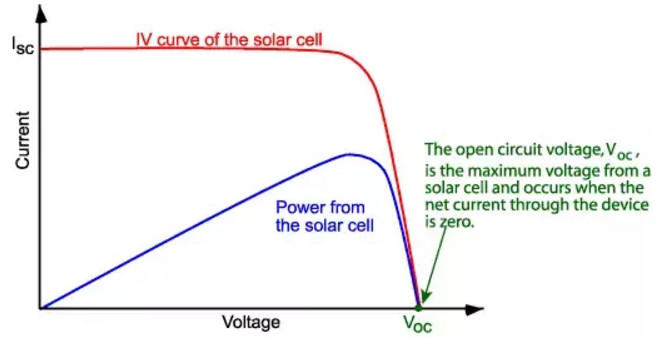
\includegraphics[width=0.36\textwidth]{Figures/MPPT.png}
\caption{Maximum power point tracking \cite{MPPT}}
\label{fig:mppt}
\end{wrapfigure}
The voltage at which the peak of the PV curve occurs is the voltage at which the maximum power is achieved. When external factors change such as temperature, light intensity and spectrum of the light, it causes the I-V and P-V curves to change \cite{vidmppt}. Under standard conditions the MPP of the solar panel in question occurs at 18.21V and 0.28A. To calculate the efficiency of the solar panel you take the radiance of the light shining on the module and multiply it by the area of the module. This is the ideal maximum power for that light. To get efficiency divide the previous answer by the power output. In general solar panels have an efficiency of 20\%\cite{eff}. 



\label{sec:STC}
The Standard Test conditions used to test the SLP005-12 solar panel is a light that emits 1000W per square meter and the light used had an AM of 1.5. The tests were completed at 25$^{\circ}$C.The Standard Testing conditions are parameter that all solar panel producers use to define the performance of their solar equipment.





\begin{table}[!htb]
        \centering
        \footnotesize
        \caption{Solar Panel Measurements}
         \begin{tabular}{lrrrr}
          \toprule
             & $V_{O.C}$ & $I_{S.C}$ & $V_{pmax}$ \\
             &  [V]  & [mA] & [V]\\
          \midrule
          Theroretical per cell & 0.6      & 340 & 0.472 \\
          Datasheet  per module &  21.6      & 340 & 17 \\
          Measured dark       & 1.1 & 0 \\
          Measured upside-down  19.19      & 7.8 & 1.0 \\
          Measured oblique       & 19.7 & 33 \\
          Measured facing        & 22.66 & 178.3 \\
          \bottomrule
        \end{tabular}
     \label{tab:PVresults}
\end{table}

%%%%%%%%%%%%%%%%%%%%%%%%%%%%%%%%%%%%%%%%%%%%%%%%%%%%%%%%%%%%%%%%%%%%%%%%%%%%%%%%%%%
\section{Lead Acid Battery}
\label{sec:Bat Intro}


\label{sec:batchar}
The battery capacity of a Lead acid battery can not be used from 100\% to 0\% but instead the battery data sheet discharges to a minimum of 1.8V per cell (5.4V). The battery in our use case is rated for 4.0Ah@20hr-rate to 1.80V which means that it was able to discharge for 20hr with a load of 0.2A until the voltage of each cell reaches 1.8V. The capacity of a lead acid battery is affected by a number of external factors such as temperature. Higher temperatures will increase capacity at the cost of accelerating ageing of the battery and lower temperatures will decrease the battery capacity  \cite{PVEducation}.

 Batteries also have an internal resistance, in our case 45m\textohm. This internal resistance will have the effect of heating the battery up. The internal resistance of the battery increases with lower temperatures and decreases with higher temperatures[2]. The battery used in E344 has a self discharge of 3\% per month at room temperature. The internal resistance can also cause a voltage drop \cite{BatteryUniversity} at the terminals when the battery is connected to a load, this can be seen in figure \ref{fig:discharge}.


\label{sec:BatteryCharging}
\begin{wrapfigure}{l}{0.4\textwidth}
\centering
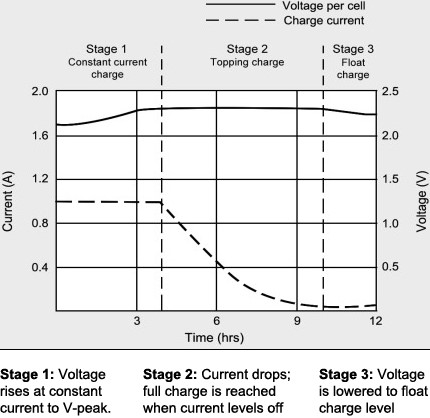
\includegraphics[scale=0.4]{Figures/cc.jpg}
\caption{Charging states of lead acid battery \cite{RS}}
\label{fig:states}
\end{wrapfigure}
 Battery charging tends to take on three different stages, these three stages can be referred to as bulk, absorption and float\cite{CC}.In the bulk charging stage the current is held at a constant amount and the voltage increases. For our battery this means 0.2-0.3C until the voltage reaches 6.75V\cite{RS}. The bulk stage includes the highest charging rate. During the absorption stage the voltage remains constant and the current decreases which leads to a decreasing charge rate. For our battery this means 0.1C until the voltage reaches 7.2V\cite{RS}. At the the end of the absorption stage the battery is at 100\% capacity. The next stage of charging is float charging where the voltage is decreased slightly (in our case to 6.75 - 6.9) and the current is at approximately 1\% of the battery capacity, this charging state is used to keep the battery charged indefinitely \cite{CC}. All these different states can be seen in figure \ref{fig:states} 






\label{sec:Discharge}
\par The C rating is a measurement of the rate at which a battery will discharge relative to its maximum capacity\cite{MIT}. 
\begin{wrapfigure}{l}{0.57\textwidth}
\centering
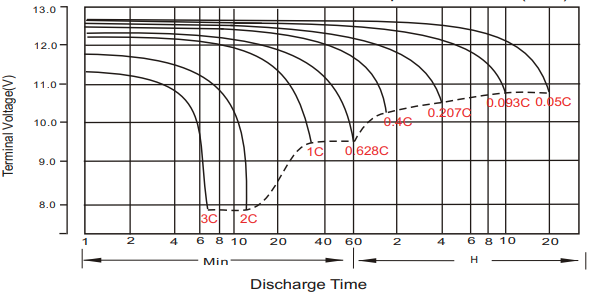
\includegraphics[scale=0.5]{Figures/fig2.png}
\caption{Discharge Characteristics \cite{Charging-Lead}}
\label{fig:discharge}
\end{wrapfigure}
 As the C rating decreases the run time does not increase linearly (refer to figure \ref{fig:discharge}), the reason for this is because a higher discharge rate causes the battery to lose energy to heat as more current flows through the internal resistance \cite{pSonic}. At higher discharge rates the terminal voltage is lower due to the internal resistance causes a voltage drop.


%%%%%%%%%%%%%%%%%%%%%%%%%%%%%%%%%%%%%%%%%%%%%%%%%%%%%%%%%%%%%%%%%%%%%%

\section{Fuse Characteristics}\label{sec:fuse_lit}
In this section, the different characteristics of the blade fuse that is being used is discussed. A fuse has a \textbf{current rating} which refers to the nominal current that the fuse can handle although it is recommended that the current at an ambient temperature of 25\textdegree C not be higher than 75\% of this value \cite{LF}. Fuses operate by blowing when current higher than the nominal rated current flow through the fuse. For this reason when the ambient temperature increases, the current required to reach a point where the fuse will melt is lower than it would be for lower ambient temperatures. This can be seen in figure \ref{subfig:temp} line "B". Current and time have an inverse relationship as can be seen in figure \ref{subfig:c-t}, this means that for higher currents the fuse will blow faster.


 \begin{figure}[!htb]
 \footnotesize
 \centering
    \begin{subfigure}[]{0.42\textwidth}
              \centering
  		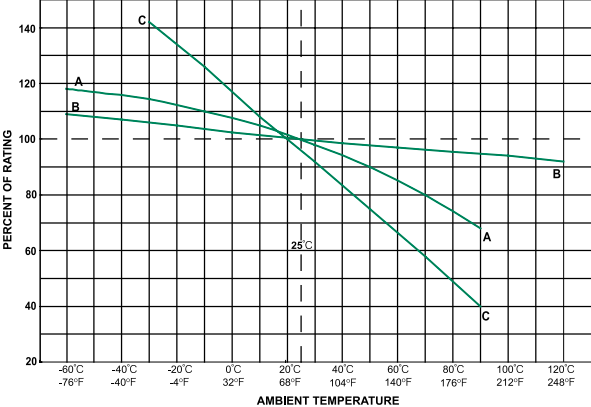
\includegraphics[width=1\linewidth]{./Figures/temperature.png}
		    \caption{} \label{subfig:temp}
     \end{subfigure}
     \begin{subfigure}[]{0.3\textwidth}
             \centering
  		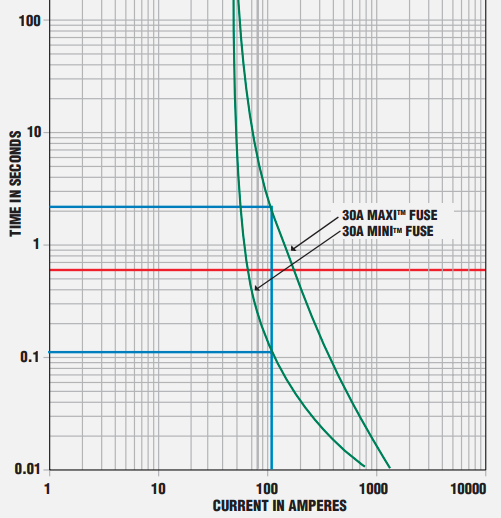
\includegraphics[width=1\linewidth]{./Figures/c-t.png}
		   \caption{ } \label{subfig:c-t}
     \end{subfigure}
   \caption[{Fuse Characteristics}]{Fuse Characteristics Relating to blow time   (a)  Current Rating versus Ambient Temperature\cite{LF} (b)  Blow time vs Current \cite{LF2} }
    \label{fig:two}
 \end{figure}



\chapter{System Design}\label{Lit:sysDesign}
%%%%%%%%%%%%%%%%%%%%
\section{Charging circuit overview}
The charging circuit structure can be seen in figure \ref{fig:A2block} as the green highlighted blocks. The 12V supply and the solar panel will connect directly to the linear regulator. The linear regulator is the part of the system that will be tuned to achieve the adequate current limiting, voltage and thermal specifications. The charging circuit will then be intercepted by the high side switch so that the charging can be controlled by a logic high or low to the switch. 

\begin{figure}[!htb]
\centering
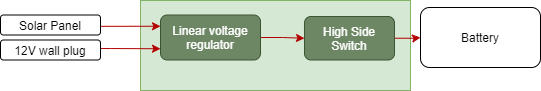
\includegraphics[scale=0.5]{./Figures/A2}
\caption{Charging System Block Diagram}
\label{fig:A2block}
\end{figure}

%%%%%%%%%%%%%%%%%%%%%%%
\section{Under Voltage and Over Current circuit overview}
The circuit structure can be seen in figure \ref{fig:A3block} as the yellow highlighted blocks. The goal of this circuit is to disconnect the battery from the load when the voltage is below a certain voltage and then to reconnect the battery when the voltage is above a certain voltage. The circuit will also protect the battery from abnormally high charging currents with a fuse. The Schmidt trigger block manages the logic of whether the switch should be on or off. This decision is then conveyed to the high side switch which then implements the connection or disconnection of the battery from the load. In order for the Schmidt trigger to work it requires 5V which will be supplied through a regulator from the battery.

\begin{figure}[!htb]
\centering
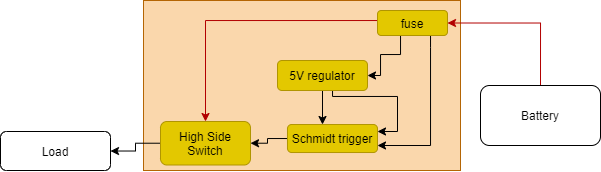
\includegraphics[scale=0.5]{./Figures/A3}
\caption{Under Voltage System Block Diagram}
\label{fig:A3block}
\end{figure}

%%%%%%%%%%%%%%%%%%%%%%%%%%%%%%%
\section{Current sense circuit overview}
The current sense circuit structure can be seen in figure \ref{fig:finalblock} as the purple highlighted blocks. The current sense circuit connects the two previous system block diagrams to make up the final block diagram.  The current sense circuitry was added at its position after the load so that the current it will measure is the current discharging from the battery or charging into the battery. In order to operate the current sense amplifier will require a 5V from the 5V regulator.  The current sense amplifier will be used to produce voltage between 0V and 5V that will correspond proportionally to the current in a designed range of 3V. The current sense amplifier will amplify very small voltages across the current sense resistor. The load can also be connected and disconnected with the help of the designed low side switch. The output of the current sense amplifier will be prone to noise from the 12V wall plug as well as the 5V regulator. In order to fix this a output filter will be required at the output of the current sense amplifier. The directions of the arrows in the block diagrams show the direction that current flow will be enforced. This means schottky diodes will be used at the solar panel the 12V wall plug as well as the output of the charging circuit. 
%%%%%%%%%%%%%%%%%%%%%%%%%%%%%%%%

\begin{figure}[!htb]
\centering
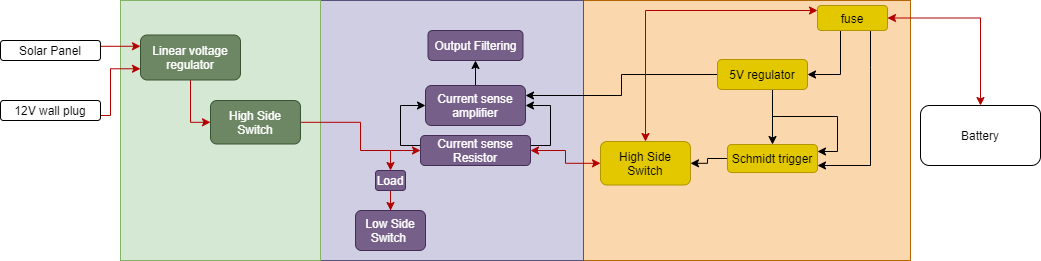
\includegraphics[scale=0.45]{./Figures/A5}
\caption{Complete System Block Diagram}
\label{fig:finalblock}
\end{figure}

%%%%%%%%%%%%%%%%%%%
\chapter{Design Details}\label{Lit:desDetails}

\section{LM317 Regulation}
\label{sec:regulation}
The voltage regulation as well as the current limiting feature can be achieved with the LM317 regulator with the use of an application circuit. The LM317 is a linear regulator which means that it uses linear components such as resistors to achieve required variations, thus it is constantly dissipating power. A switching regulator makes use of PWM  to get the required variation. Because PWM means it is turns on and off it dissipates less power than a linear regulation \cite{SvsL}. Figure \ref{fig:app} is the application circuit that will be used in the design process to achieve the constant voltage and current limiting specifications. The resistor values will be redesigned. The regulator works on the basis that the difference between the output terminals and adjust terminals is a "fixed" voltage. The current flowing into $I_{adj}$ is typically 50\textmu{}A but can be a maximum of 100 \textmu{}A\cite{STM}.
The following equation \ref{eq:vo} is obtained from the data sheet \cite{STM} and correspond to figure  \ref{fig:app}.

\begin{equation}
    V_{O-reg}=V_{ref-reg}\times(1+\frac{R_2}{R_1})+(I_{adj})\times (R_2)
    \label{eq:vo}
\end{equation}

    \begin{equation}
         V_{O-reg}-V_{adj}=1.25V
         \label{eq:vref}
    \end{equation}

\subsection{Voltage regulation}
A voltage of 7.2V is designed for using equation \ref{eq:vo}. This voltage is slight lower than the 7.35V  ($2.45\times3$) specified in the data sheet. It can be considered a safety factor.  
\begin{center}
    $\frac{R_2}{R_1}=\frac{7.2}{1.25}-1=4.76$
\end{center}

The resistor values used should be kept low so that the current flowing through $R_1$ and $R_{2}$ is significantly larger than $I_{adj}$. If this is done then $I_{adj}$ can be neglected. $R_{2}$ is chosen to be 1000\textohm. Therefore $R_{1}$ will be 210\textohm. Refer to figure \ref{fig:app}.


\begin{center}
    
    $\frac{7.2}{R_1+R_2} = 5mA>>$100\textmu A
\end{center}
Because 5mA is 50 times larger than the maximum, the $I_{adj}$ can be assumed to be negligible as it will have minimal effect on the calculations.

\subsection{Current limit}

The current limiting was implemented by calculating a value for $R_4$ (refer to \ref{fig:circuit}). The maximum current that was designed for was 400mA. This value was chosen because the battery data sheet recommends 0.1C for charging which equates to 400mA \cite{RS}. This current will be designed flow when the battery is at its depleted voltage of 6V. To determine $R_s$ $V_O$ must be calculated when $V_{bat}$=6V. Using the calculated $V_0$ the resistor $R_s$ is designed for the desired current.



\begin{center}
 $V_{schottky}=0.4V$

\end{center}
\begin{center}

    $V_{adj} = (6+V_{schottky})-\frac{(6+V_{schottky})\times R_1}{R_1+R_2}$=5.29V
 
\end{center}
\begin{center}

    $V_{O-reg}= 1.25+V_{adj}$=6.539V (refer to equation \ref{eq:vref})
    
    
\end{center}
\begin{center}
    $R_s=\frac{V_{O-reg}-(V_{bat}+V_{schottky})}{400mA}=\frac{6.539V-6.4V}{300mA}=0.347$\textohm
\end{center}
The biggest flaw with this method is that $V_{schottky}$ voltage is not accurate. Another problem will be that achieving a resistance of 0.347\textohm \ will be very inaccurate.

%%%%%%%%%%%%%%%%%%%%%%%%%%%%%%%%%%%%%%%%%%%%%%
\subsection{Thermal analysis}
\begin{wrapfigure}{l}{0.25\textwidth}
\centering
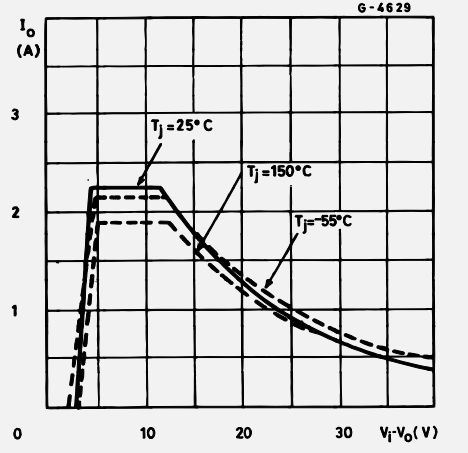
\includegraphics[scale=0.2]{Figures/temp.png}
\caption[{Output current vs. input-output
differential voltage for different junction temperatures}]{Output current vs. input-output
differential voltage for different junction temperatures\cite{STM}}
\label{fig:temp}
\end{wrapfigure}

As the junction temperature increases the output current will decrease for the same $V_i-V_{O-reg}$\cite{STM} (refer to \ref{fig:temp}). All thermal resistance values used can be found at \ref{tab:Thermal values}.



\begin{equation}
    T_j-T_a=P_{tot}\times(\theta_{j-a})
    \label{eq:woSink}
\end{equation}

\begin{equation}
    T_j-T_a=P_{tot}\times(\theta_{j-s}+\theta_{s-a})
    \label{eq:wSink}
\end{equation}

The most power our regulator will dissipate is:
\begin{center}
    $0.3A\times(12V-6.539V)=1.64W$
\end{center}


Without a heat sink, at an ambient temperature of 25\textdegree C the junction temperature will be(refer to eq. \ref{eq:woSink}):

\begin{center}
$T_j=1.64W\times(50$\textdegree C/W$)+25$\textdegree C=107\textdegree C. 
\end{center}

With the heat sink, at an ambient temperature of 25\textdegree C the junction(refer to eq. \ref{eq:wSink}):
\begin{center}
    $T_j=1.64W\times((5+20)$\textdegree C/W$)+25$\textdegree C=66\textdegree.
\end{center}

We want out current to be predictable and close to the value calculated, the heat sink enables the calculation to be more accurate. The maximum operating temperature of the regulator is 125\textdegree C \cite{STM}. 107\textdegree C is quite close and I would definitely recommend that the heat sink is used. For a higher input voltage the regulator could break without a heat sink. 


\begin{figure}[!htb]
\centering
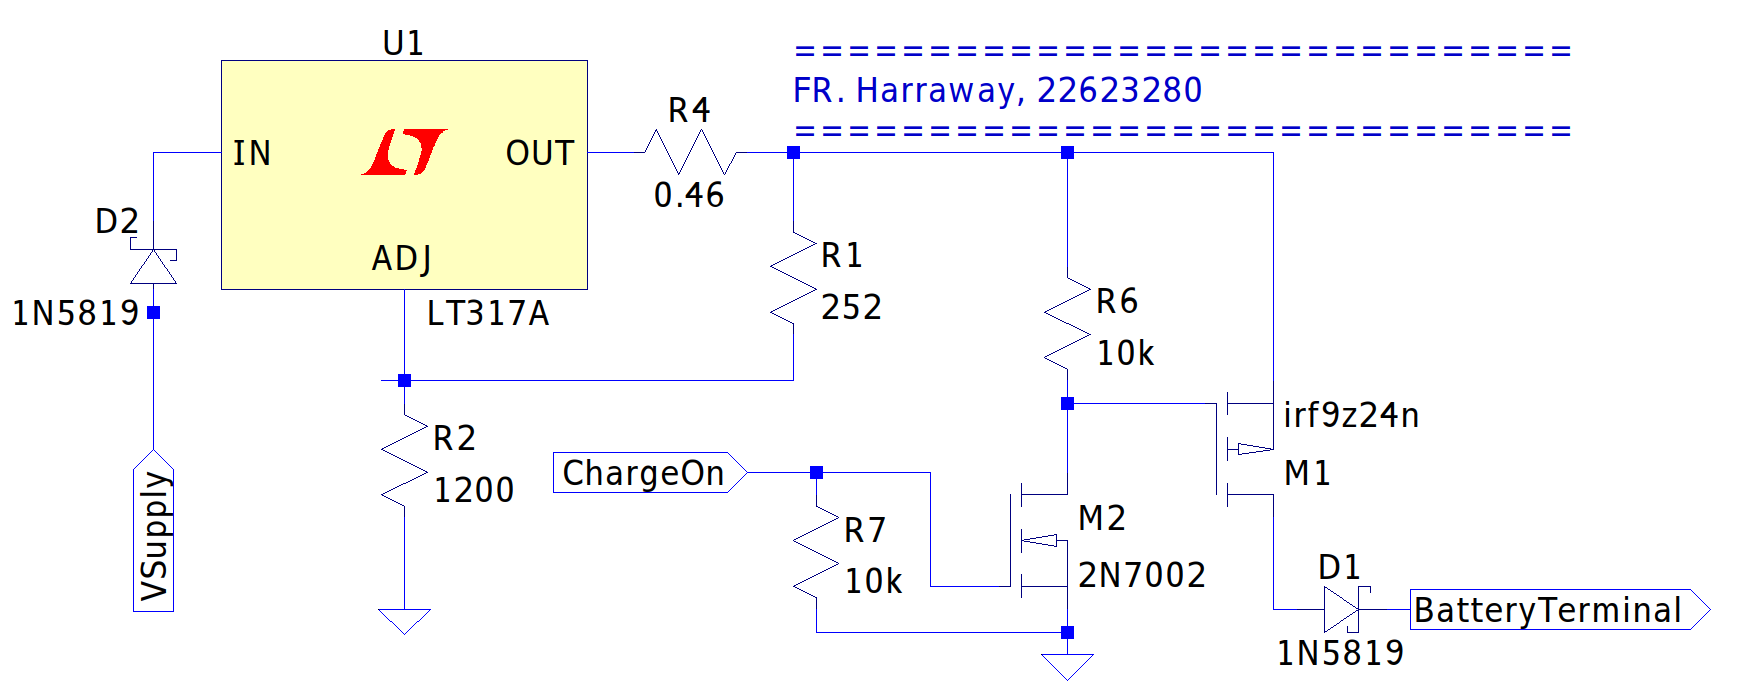
\includegraphics[scale=0.3]{Figures/FinCirc.png}
\caption{Charging Circuit with high side switch implemented }
\label{fig:circuit}
\end{figure}

%%%%%%%%%%%%%%%%%%%%%%%%%%%%%%%%%%%%%%%%%%%%%%%%%%%%%%%%%%%%%%%%%%%%%%%%%%%%%%%%%%%%%%%%%%%%%%%%%%%%%%%%%%%%%%%%%%%%%%%%%%%%%%%%%%%%%%%%%%%%%%%%%%%%%%%%%%%%%%%%%%%%%%%%%%%%%%%%%%%%%%%%%%%%%%%%%%%%%%%%%%

\section{High side switch on supply side}
\label{sec:high}
%%%second part
Switches are often used to control the flow of current within a circuit. In this report only enhancement mode MOSFETs will be used. The MOSFETs we are using have 3 terminals, gate, source and drain as can be seen in figure \ref{fig:mosfets}.\begin{wrapfigure}{l}{0.5\linewidth}
\centering
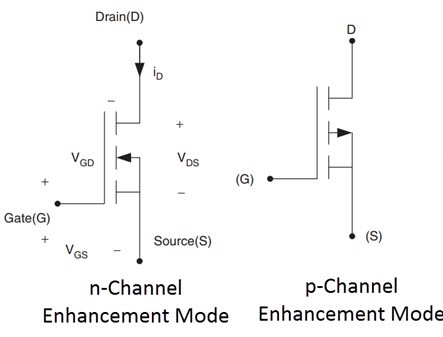
\includegraphics[height=4cm]{Figures/mosfetX.jpg}
\caption{The different MOSFET configurations}
\label{fig:mosfets}
\end{wrapfigure} For a NMOS chip the current will flow from the drain to source when it is in its \textbf{ON} state whereas for a PMOS the drain current will flow from the source to the drain. For the NMOS to turn on a positive voltage across the gate and the source must be applied that is larger than a certain threshold (refer to figure \ref{subfig:NMOS-graph}). For a PMOS the same is true however the voltage is instead negative (refer to figure \ref{subfig:PMOS-graph}).



\begin{figure}[!htb]
 \footnotesize
 \centering
    \begin{subfigure}[]{0.55\textwidth}
              \centering
  		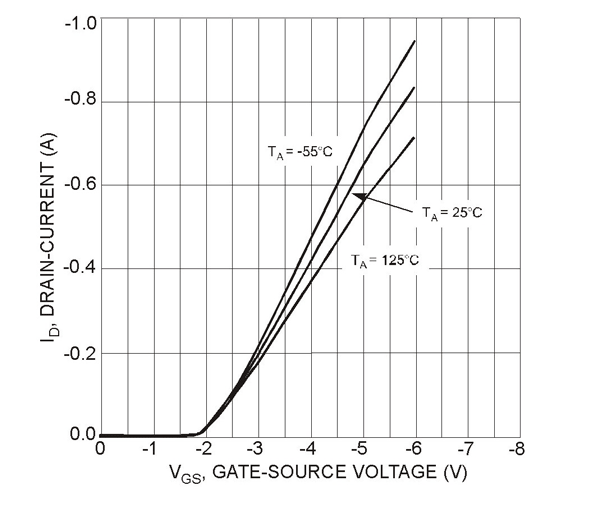
\includegraphics[width=0.5\linewidth]{./Figures/PMOS.png}
		    \caption{} \label{subfig:PMOS-graph}
     \end{subfigure}
     \begin{subfigure}[]{0.4\textwidth}
             \centering
  		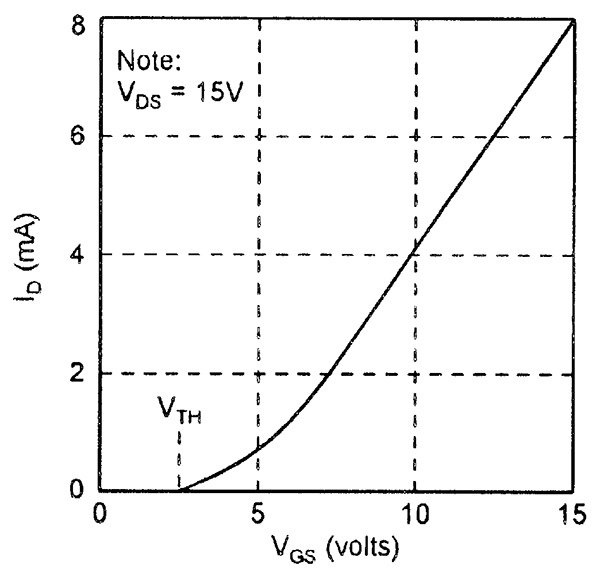
\includegraphics[width=0.6\linewidth]{./Figures/NMOS.jpg}
		   \caption{ } \label{subfig:NMOS-graph}
     \end{subfigure}
   \caption[{$V_{GS}$  vs  $I_{D}$}]{Turn on voltages for NMOS and PMOS (a)  PMOS \cite{PMOS}(b)  NMOS\cite{NMOS}  }
    \label{fig:simulation_results_box}
 \end{figure}




 When designing the switch the considerations taken into account was the fact that the PMOS can handle in excess of amps \cite{PMOS} whereas the NMOS can only handle 200mA\cite{NData}. For this reason the NMOS is used to switch the PMOS on. The way that this is achieved is by turning the NMOS on with a logic high of 5V, when the NMOS is on current flows through $R_1$ and $R_2$ (refer to figure \ref{fig:high}) and this causes there to be a voltage over the source and gate of the PMOS. This voltage needs to be greater than 4V and less than 20V in order for the PMOS to turn on and function without breaking \cite{PMOS}.The NMOS has a maximum threshold voltage of 3V. The 5V will be enough to turn it on \cite{NMOS}. A resistor is also placed between the gate of the NMOS and ground to prevent the gate from floating. 
 
\begin{itemize}
 \item To prevent current from the load from flowing back into the supply a schottky diode is placed in series with the load.
\item To ensure that all the 25V is not across the PMOS $V_{SGp}$ terminals the voltage is divided using $R_1$ and $R_2$ (refer to figure \ref{fig:high}).
\item The magnitudes of the resistors used were decided mainly to restrict excessive current flow through the resistors,$\frac{5}{10k}$=0.5mA or $\frac{25}{20k}$=1.25mA which is relatively small.
\end{itemize}



    \begin{equation}
        I_{Dn}=\frac{R_1+R_2}{V_{supply}-V_{DSn}}
        \label{eq:curr}
    \end{equation}

\begin{equation}
V_{SGp}=V_{R1}=I_{Dn}*R_1   
\label{eq:one}
\end{equation}



    $R_{1}=10k$\si{\ohm} \ $R_{2}=10k$\si{\ohm}\ $V_{supply}=25V$. If $V_{DSn}\approx0 $ for $ V_{GSn}=5V$  then using eq.\ref{eq:curr} $I_{Dn}=1.25mA$.Using eq.\ref{eq:one} $V_{SGp}=12.5V$\ , this is larger than 4V and smaller than 20V and will "turn on" the PMOS transistor without damaging it. 

 


\begin{figure}[!htb]
\centering
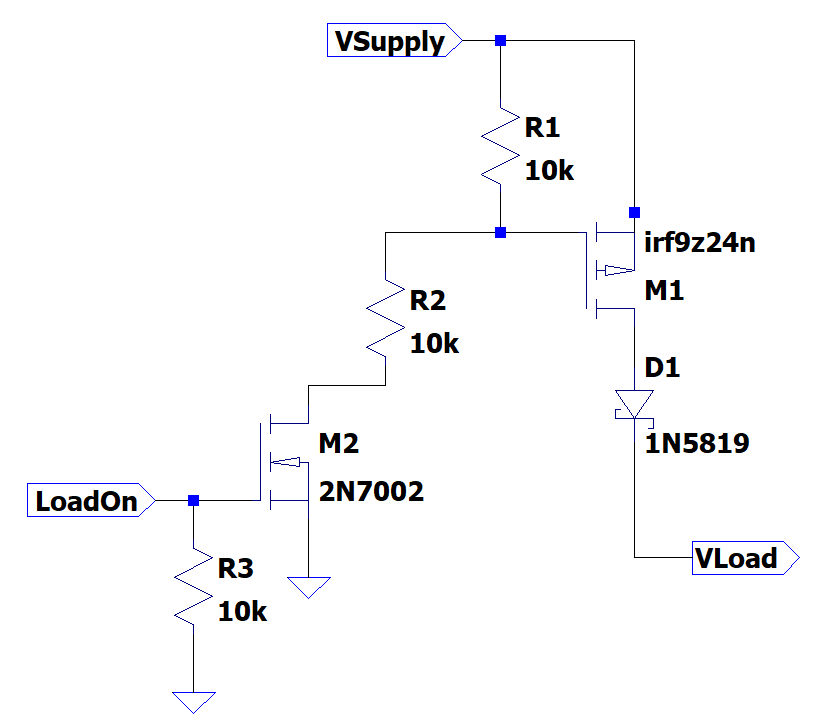
\includegraphics[scale=0.28]{Figures/Highside.png}
\caption{High side\textbf{} switch circuit}
\label{fig:high}
\end{figure}



%%%%%%%%%%%%%%%%%%%%%%%%%%%%%%%%%%%%%%%%%%%%%%%%%%%%%%%%%%%%%%%%%%%%%%%%%%%%%%%%%%%%%%%%%%%%%%%%%%%%%%%%%%%%%%%%%%%%%%%%%%%%%%%%%%%%%%%%%%%%%%%%%%%%%%%%%%%%%%%%%%%%%%%%%%%%%%%%%%%%%%%%%%%%%%%%%%%%%%%%%%
\newpage
\section{Over current protection}
From the battery's perspective, it will be able to discharge 60A for 5 seconds as an absolute maximum \cite{RS}. The battery also has a maximum recommended charging limit of 1.2A \cite{RS}. We will not be charging at 1.2A, we will be charging at approximately 400mA (I chose 300mA refer to \ref{sec:regulation}).

The load we are going to use will be made up of 5 ultra bright LEDs. The peak forward current of one of these LEDs is 100mA \cite{LED}. This means that for the peak case, just the load will use 500mA of current, however we will be designing for the typical 20mA per LED with current limiting resistors (refer to section \ref{sec:loswide}). This is then equated to 100mA for the entire load.

From the previously mentioned information we have 4 different current limit values. Two of these values are limits regarding the battery's limits and 2 are limits regarding what the circuit should charge/discharge. The fuse will be connected between the battery and the complete circuit, all current charging/discharging from the battery will flowing through the designed fuse.

The battery's limits are well above what the circuit will require, therefore the upper limit of the circuit charging will be used as the reference for the design. I then doubled the 400mA charging current to set the fuse for an abnormal condition. If 800mA of current flow then something is not working correctly and the battery should stop discharging. The closest fuse we have to this is 1A. 

%%%%%%%%%%%%%%%%%%%%%%%%%%%%%%%%%%%%%%%%%%%%%%%%%%%%%%%%%%%%%%%%%%%%%%%%%%%%%%%%%%%%%%%%%%%%%%%%%%%%%%%%%%%%%%%%%%%%%%%%%%%%%%%%%%%%%%%%%%%%%%%%%%%%%%%%%%%%%%%%%%%%%%%%%%%%%%%%%%%%%%%%%%%%%%%%%%%%%%%%%%
\newpage
\section{Undervoltage protection}
In the design below the concepts of a op amp voltage comparator is used. A comparator will amplify the difference of the two terminals.
\begin{figure}[!htb]
\centering
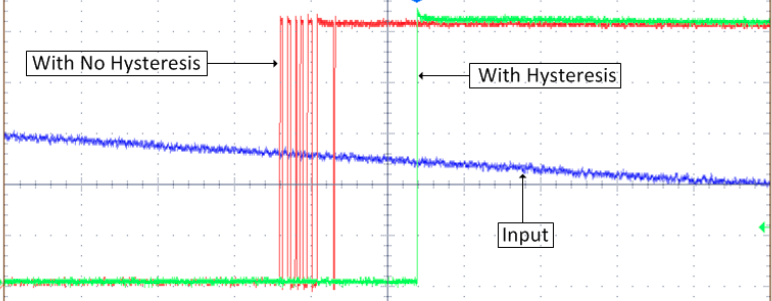
\includegraphics[scale=0.2]{./Figures/hyst}
\caption[{Op-Amp with hysteresis implemented compared with no hysteresis}]{Op-Amp with hysteresis implemented compared with no hysteresis \cite{TexHyst}}
\label{fig:hyst}
\end{figure}
A problem with the standard comparator op-amp configuration is that if a noisy signal is placed at the input of the op-amp it could cause the op amp output to switch between the two supply rails in a short period of time leading to a signal as can be seen in figure \ref{fig:hyst}. A op amp with hysteresis means that the op amp has positive feedback from the output and this causes the output of the op amp to switch from rail to rail at two voltages $V_{TU}$ and $V_{TL}$ , refer to \ref{fig:schmidt2}.




\subsection{5V rail}
In the circuit that was used in the final design an LM2940 regulator was chosen over a LM7805 regulator because of the respective drop out voltages of 0.5V \cite{TexReg} and 2V\cite{TexRegpos}. This is important because the voltage input to the regulator can be as low as 6V (battery terminal) and that would mean that the LM7805 would have a regulated voltage of below 5V. The LM7805 is able to output a maximum recommended amperage of 1.5A whereas the LM2904 only has a recommended output current of 1A \cite{TexReg}\cite{TexRegpos}. The LM2940 does have a typical quiescent current of 10mA which is ideal as we are designing for this current or less than 10mA \cite{TexReg}. 

\subsection{High-side switch}

%%%second part
The fundamental design is the same as in section \ref{sec:high}, the only difference is the lack of $R_2$ and the schottky diode. $R_2$ is not need to decrease the voltage $V_{GS}$ at the PMOS and no current flow restrictions are needed from the schottky diode. The high side switch is used at the position specified in figure \ref{fig:A3block}, it must be able to control the discharge of the battery but not restrict charging from the charging circuit. To ensure that this would not be an issue the reverse current of the PMOS was found in the respective data sheet to be -12A \cite{PMOS}.


\subsection{Voltage monitoring with hysteresis design}
 The positive supply rail of the op amps in this design will be connected to the 5V regulator and the negative supply rails will be grounded($V_{DD}$ and $V_{SS}$). When designing the input voltages to the op amp it was decided to step the voltages down using voltage division because if the battery terminal (max of 7.2V) is connected and a 0V is connected then the differential voltage maximum will be exceeded. The circuit that was built was based off the non inverting Schmidt trigger as can be seen in figure \ref{fig:schmidt2} \cite{Schmidt}.
 
 \begin{figure}[!htb]
 	\centering
 	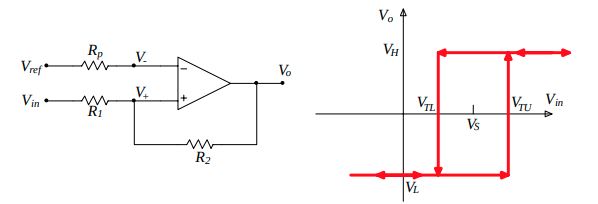
\includegraphics[scale=0.5]{./Figures/schmidt}
 	\caption[Non inverting Schmidt trigger]{Non inverting Schmidt trigger\cite{Schmidt}}
 	\label{fig:schmidt2}
 \end{figure}

  This configuration compares an input voltage with a constant reference voltage and the output will switch to the positive supply rail at an input voltage of $V_{TU}$ and to the negative supply rail at $V_{TL}$ (refer to \ref{fig:schmidt2}). A divided voltage from the 5V regulator is used as a reference voltage because it will remain "constant". The suitable $V_{ref-Schmidt}$ is calculated below and $V_{ref-Schmidt}$ is connected to a voltage follower op amp to prevent the positive feedback from affecting the input voltage. The battery voltage is divided to be 4.5V ($\frac{7.2*100}{100+60}$=4.5V) at the op amp terminal using $R_7$,$R_{10}$ and $R_8$(refer to figure \ref{fig:under}). With a battery terminal voltage of 6.2V the voltage at the op amp will be $V_{TU}=3.875$V and with 6V the voltage will be $V_{TL}=3.75$V. $V_L$ (approx zero volts) is the low output of the Schmidt trigger and $V_H$ is the high output of the Schmidt trigger(approx 5V). Equations below are for a non-inverting Schmidt trigger. \textbf{The equations are derived extensively in Appendix C}.



\begin{center}
	$\frac{V_{TU}-V_{TL}}{(V_{H}-V_L)}=\frac{R_1}{R_2}$  
\end{center}

\begin{center}
	
$	V_{REF}=\frac{V_{TL}\times (R_2)}{R_1+R_2}+\frac{V_{H}\times R_1}{R_1+R_2}$
\end{center}




Using the above equations the $\frac{R_1}{R_2}$ ratio is found to be $\frac{1}{40}$.$R_2$ is chosen to be 190k\textohm which results in $R_1$= 4.75k\textohm. The closest lab resistor is 4.7k\textohm. With our resistor values now defined $V_{REF}$ can be calculated to be 3.78V. The relevant voltage division can be found in figure \ref{fig:under}



\begin{figure}[!htb]
\centering
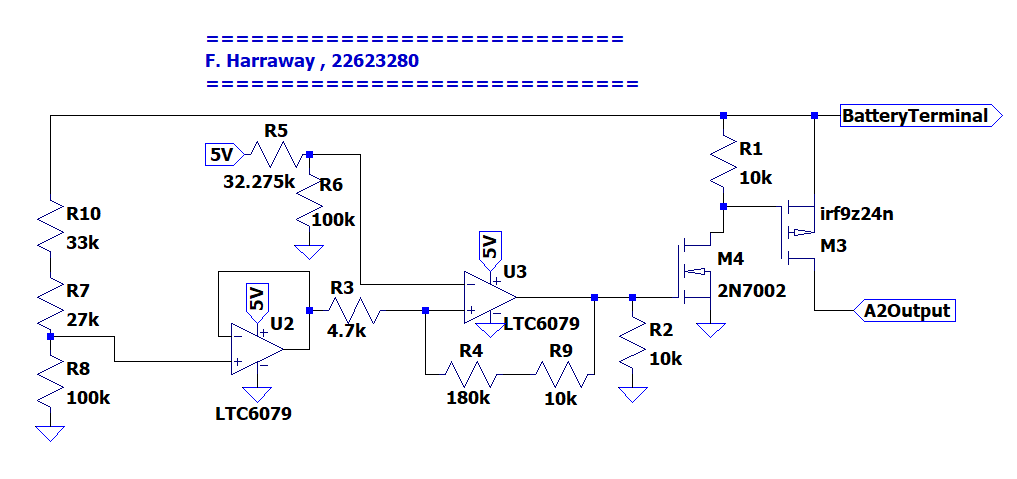
\includegraphics[scale=0.5]{./Figures/undervoltage}
\caption{Circuit diagram of under voltage circuit connected to the high side switch and the output of the previous assignment as well as the battery terminal}
\label{fig:under}
\end{figure}



\begin{table}[!htb]
	\centering
	\footnotesize
	\caption[Undervoltage circuit op amp requirements]{Undervoltage circuit op amp requirements \cite{MCP}}
	\begin{tabular}{lrrrr}
		\toprule
		& $Min$ &$Max$&$Designed$\\
		&[V]&[V]&[V]\\
		\midrule
		All op amps Difference between supply rails $V_{DD} - V_{SS}$ & -& 7  &5   \\
		U2 Common mode voltage $(\frac{V_+ + V_-}{2}-V_{SS})$ &  -0.3&5.3&3.75-4.5\\
		U2 Input voltages to $V_-$ and  $V_+$   &  -1    &6& 3.75-4.5 \\
		
		
		U3 Common mode voltage $(\frac{V_+ + V_-}{2}-V_{SS})$ &  -0.3&5.3&3.72-4.12\\
		U3 Input voltages to $V_-$ and $V_+$  &  -1    &6&0-4.51 \\
		U3 Differential Voltage $ (|V_+ - V_-|)$ & -& 7& 4.51   \\
		
		\bottomrule
	\end{tabular}
	\label{tab:MCPunder}
\end{table}

From table \ref{tab:MCPunder}, all op amps are operating within working ranges.


%%%%%%%%%%%%%%%%%%%%%%%%%%%%%%%%%%%%%%%%%%%%%%%%%%%%%%%%%%%%%%%%%%%%%%%%%%%%%%%%%%%%%%%%%%%%%%%%%%%%%%%%%%%%%%%%%%%%%%%%%%%%%%%%%%%%%%%%%%%%%%%%%%%%%%%%%%%%%%%%%%%%%%%%%%%%%%%%%%%%%%%%%%%%%%%%%%%%%%%%%%
\newpage
\section{Current sense}
The bidirectional current sense amplifier is an op amp that is setup internally as can be seen in figure \ref{fig:data}. This internal circuitry is necessary because the resistors used need to be very accurate in order for current sensing to be accurate \cite{utube}. Another reason that the tsc213 is being used over a conventional op amp is because this device has a absolute differential voltage of 26V and a common mode voltage range of $gnd-0.3V$ to 26V. This is important for us because we can have differential voltages of up to 7.2V ($7.2-0$) and common mode voltages of about 7.2V which would not work with the previously used MCP op amp. We do not want to step down the voltages as we did previously because it would not be accurate for the current measurements. The current sense amplifier will have its positive and negative inputs connected across a shunt resistor, the current sense amplifier will then amplify this difference by 50 (refer to \ref{fig:data}).



When designing the current sense amplifier the current range that will be used should be considered. The most current that should be discharged from the battery should be 100mA. The maximum that the battery should charge at is 400mA. The current range was then determined to be $-150mA<I_{range}<450mA$, the additional 50mA was added as a safety factor to ensure the tsc213 does not breach the 0-5V output range. We do not want to breach this range because it could damage the micro controller to which the output of the tsc213 will be connected. The output voltage range will be dependant on the differential voltage of the op amp and the reference voltage chosen (refer to eq \ref{eq:refeq}). The differential voltage will be dependant on the shunt resistance and the current through the shunt. The final circuit structure can be seen in figure \ref{subfig:c-s}.
\begin{equation}
    V_o=(R_{shunt}\times I_{shunt})\times50+V_{ref-cs}
    \label{eq:refeq}
\end{equation}
Using eq.\ref{eq:refeq} $R_{shunt}$ is designed to give an output voltage swing of 3V for the current sense amplifier.
\begin{center}
    $V_{swing}=((R_{shunt}\times 0.45)-(R_{shunt}\times -0.15))\times 50$. \ \ $R_{shunt}=0.1$\textohm 
\end{center}

This results in voltage range across the shunt of $-15mV<V_{shunt}<45mV$. With a 0V at $V_{ref-cs}$ the output range (using eq.\ref{eq:refeq}) would be -0.75V to 2.25V. This is not within 0V to 5V, this is where $V_{ref-cs}$ is used to place the output voltage into a desirable range. The minimum $V_{ref-cs}$ to get the output into the desired range would be 0.75V. The maximum $V_{ref-cs}$ that would place the maximum output voltage at 5V would be 2.75V (i.e. 5-2.25). The average of the maximum and minimum $V_{ref-cs}$ is then taken and found to be 1.75V. By doing this output voltage will be equally far from the upper and lower bounds of the 0V to 5V specification. To achieve this 1.75V the voltage from a 5V regulator is divided with resistors (refer to figure \ref{fig:A4circ}). \newline

To reduce the noise at the output a passive filter was designed and placed at the output of the TSC213. This can be seen in figure \ref{fig:A4circ}.The larger this capacitor the slower the response of the TSC213 output will be. If the value is too small then the output noise will not be sufficiently reduced. The passive filtering is needed because the 5V regulator as well as the 12V wall supply introduces a lot of noise into the system.

 \begin{figure}[!htb]
 \footnotesize
 \centering
    \begin{subfigure}[]{0.42\textwidth}
              \centering
  		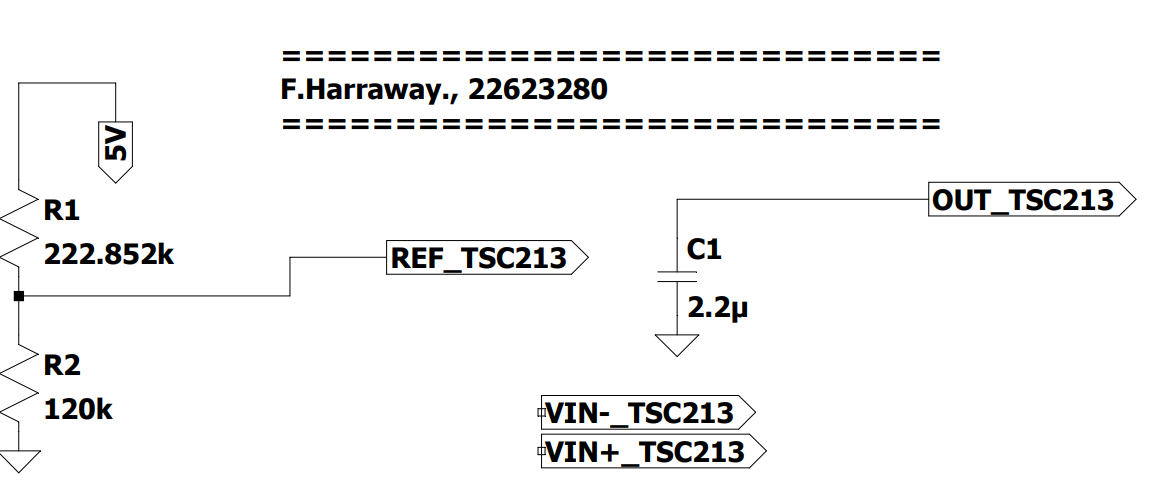
\includegraphics[width=1\linewidth]{./Figures/A4circ}
		    \caption{} \label{fig:A4circ}
     \end{subfigure}
     \begin{subfigure}[]{0.5\textwidth}
             \centering
  		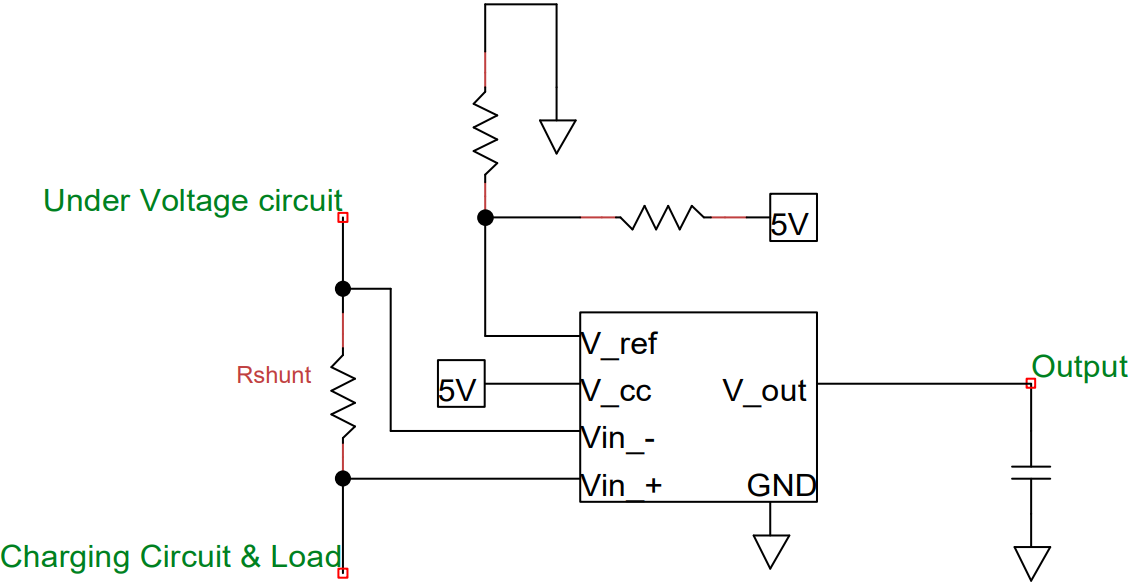
\includegraphics[width=1\linewidth]{./Figures/currentSense}
		   \caption{ } \label{subfig:c-s}
     \end{subfigure}
   \caption[{Fuse Characteristics}]{Current sense circuitry   (a) LT Spice current sense circuit (b)  Current sense circuit }
    \label{fig:C-S}
 \end{figure}




%%%%%%%%%%%%%%%%%%%%%%%%%%%%%%%%%%%%%%%%%%%%%%%%%%%%%%%%%%%%%%%%%%%%%%%%%%%%%%%%%%%%%%%%%%%%%%%%%%%%%%%%%%%%%%%%%%%%%%%%%%%%%%%%%%%%%%%%%%%%%%%%%%%%%%%%%%%%%%%%%%%%%%%%%%%%%%%%%%%%%%%%%%%%%%%%%%%%%%%%%%
\newpage
\section{Low Side Switch and Load}
\label{sec:loswide}
\label{sec:loadcontrol_lit}
In this design notable factors that will affect the design will be outlined. The load that will be used is made up of 5 LEDs that will be designed in such a way so that together 100mA is drawn. The NMOS we are going to use is able to sink a maximum continuous drain current of 200mA \cite{NData}. A low side switch means that the "switching element" is place in between ground and the load. This can be seen in figure \ref{fig:loadcirc}.

\label{sec:loadcontrol_design}
Because 100mA is the maximum current a 2n7000 NMOS chip was deemed enough to be used as a switch for the load. To "turn on" the NMOS a 5V control signal will be used. To ensure that the gate of the NMOS can not float a pull down resistor will be used. For a drain current of 100mA, according to the data sheet the $V_{DSon}$ voltage will be approximately 0.2V for a $V_{gs}$ of 5V \cite{NData}. The LED we are using has a typical forward bias voltage of 3.2V at 20mA \cite{LED}. To limit the current to 20mA ($7.2V-20mA*R_{limit}=3.2V+0.2V$) a resistor of 190\textohm \ would be ideal ,but only 220\textohm's are available in the labs. The LEDs will be in series with the current limiting resistor. The LED-resistor units will then be placed in parallel to each other (refer to figure \ref{fig:loadcirc}).

\begin{figure}[!htb]
    \centering
    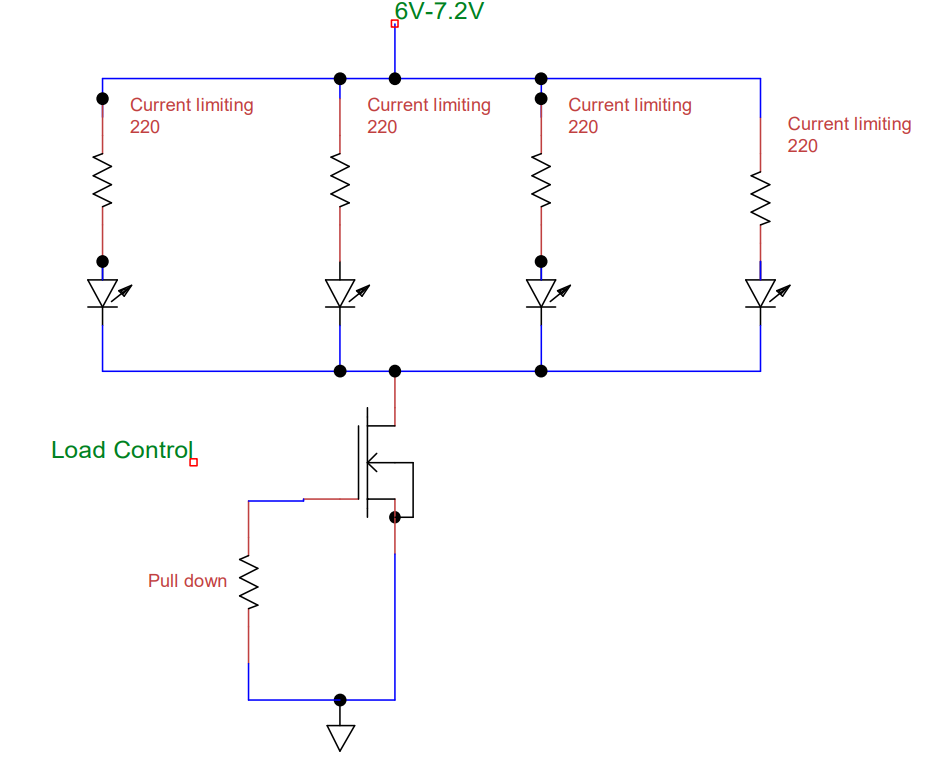
\includegraphics[width=0.4\linewidth]{Figures/loadCircuit.png}
    \caption{Load circuitry with low side switch implemented}
    \label{fig:loadcirc}
\end{figure}

\newpage
\section{Supply voltage measurement}
The Supply voltage of supply will vary from voltages of zero volt to just below 23V. To measure the supply measurement needs to converted to a voltage between zero and five volts in order for the arduino beetle to successfully read a voltage without breaking. There should be a boundary between 5V and the maximum converted voltage. To implement this a maximum voltage of 24V is designed for instead of 23V. One of the two possible supplies, the AC wall plug will introduce noise into the circuit (50Hz from the mains). This noise will likely be 50Hz which will be designed for adequately using a low pass RC filter.


\begin{center}
	$\frac{R_{10}}{R_{10}+R_9}\times24V=5V$
\end{center}
If $R_9$ is chosen to be 100k\textohm \ $R_{10}$ will be 26.3k\textohm.

\begin{equation}
f_c=\frac{1}{2\times pi\times R\times C}
\label{eq:freq}
\end{equation}
To prevent the noise of the ac wall plug from interfering with the measurement the low pass cut off filter is designed to cut off at half of 50Hz to ensure a cleaner signal. The capacitor is chosen to be 200nF. Cutting off at a lower frequency would get rid of more noise  and attenuate 50Hz noise better, however the rise time is dependant on the cut off frequency. $T_r \approx \frac{0.35}{f_c}$. For this reason the cut off frequency is not designed too low.  As an example the error that a 100mV offset on the input to the ADC will have is calculated as $\frac{100mV\times 26}{126}= V_{error}$, $V_{error}$ is then equal to 0.48V. This indicates the need for a filter.

Using eq.\ref{eq:freq} with a chosen capacitor of 200nF the required resistance for a 25Hz cut off is found to be 32k\textohm.

\begin{figure}[!htb]
	\centering
	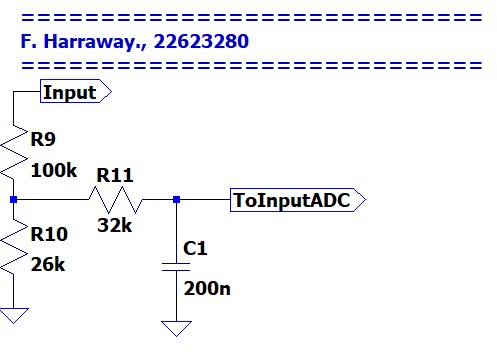
\includegraphics[width=0.26\linewidth]{Figures/A6/Supsig.jpg}
	\caption{Supply measurement circuit}
	\label{fig:supcirc}
\end{figure}


\newpage

\section{Battery voltage measurement}
In this design the battery voltage will be go through a signal conditioning process to make it readable from the perspective of an ADC. The ADC we are going to use requires a voltage between 0 and 5V. The battery voltage will vary between 6V and 7.2V if the complete system is working as designed. 

For the purpose of the design an additional 0.3V will be extended on to either side of the boundaries to give a margin for error (5.7V to 7.5V).  Using Op Amps the battery voltage will be designed to vary linearly with an output swing of 4.3V (0.5V to 4.8V). As the battery voltage increases the ADC voltage will increase. The ADC output is less than five volts in order to prevent damage to the ADC as well as the op amps. The chosen resistors are chosen to be bigger than 20k\textohm \ in order to minimise current drawn from the battery and the five volt regulator. To fit op amp spec requirements the input voltage is divided with resistors to be  four volts at the maximum designed voltage of 7.5V  as can be see in figure \ref{fig:batcirc}, this will result in a voltage of 3.04V when the battery voltage is 5.7V.

\begin{figure}[!htb]
	\centering
	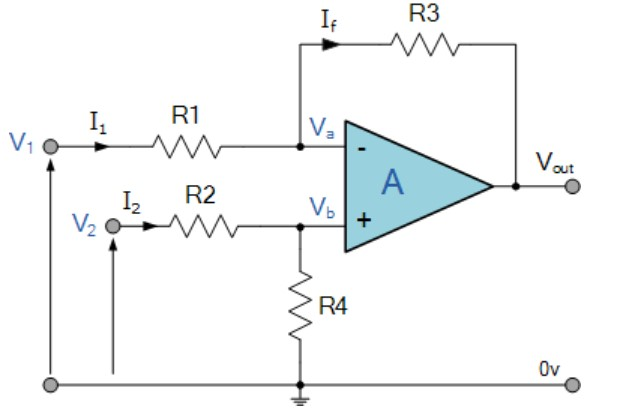
\includegraphics[width=0.27\linewidth]{Figures/A6/difamp.jpg}
	\caption[Differential amplifier op amp setup]{Differential amplifier op amp setup\cite{difAmp} }
	\label{fig:difamp}
\end{figure}

To achieve the differential amplifier setup from figure \ref{fig:difamp} is used. In this design $R_1$=$R_2$ and $R_3$=$R_4$ \cite{difAmp}. The corresponding equation is as seen in equation \ref{eq:diff}.  $V_1$ will be used as the reference voltage and $V_2$ will be our input from the battery. \textbf{The derivation can be found in Appendix D \ref{fig:derive}}.

\begin{equation}
	V_{out}=\frac{R_3}{R_1}\times(V_{2(bat)}-V_{1(ref)}) 
	\label{eq:diff}
\end{equation}

Using eq.\ref{eq:diff}, $V_{1(ref)}$ and the gain is solved for simultaneously by setting the equations for the scenarios when the battery voltage is 7.5V and 5.7V.

\begin{center}
	 $4.8V=\frac{R_3}{R_1}\times(4V-V_{1(ref)}) \ \ \ \ \ \ \ \ 0.5=\frac{R_3}{R_1}\times(3.04V-V_{1(ref)}) $\newline 
	
	$\frac{4.8V}{(V_{1(ref)}-4V)}=\frac{0.5V}{(V_{1(ref)}-3.04V)}  \ \ \ \ \ \ \ \ V_{1(ref)}=2.93V \ \ \ \ \ \ \frac{R_3}{R_1}=4.48$\newline
\end{center}


$R_3$ is then chosen to be 100k\textohm. $R_1$ is the calculated to be 22.32k\textohm. Both $V_1$ and $V_2$ need to be divided to a lower voltages 2.93V and four volts (when battery is at 7.5V), the relevant resistors for the voltage division can be seen in figure \ref{fig:batcirc}.  $V_1$ requires a buffer in between the divided battery voltage and the differential op amp to prevent the negative feedback from interfering with the input voltage. $V_2$ also requires a buffer because otherwise $R_2$ and $R_4$ will the change the effective voltage division and 2.93V would not be achieved. 

\begin{figure}[!htb]
	\centering
	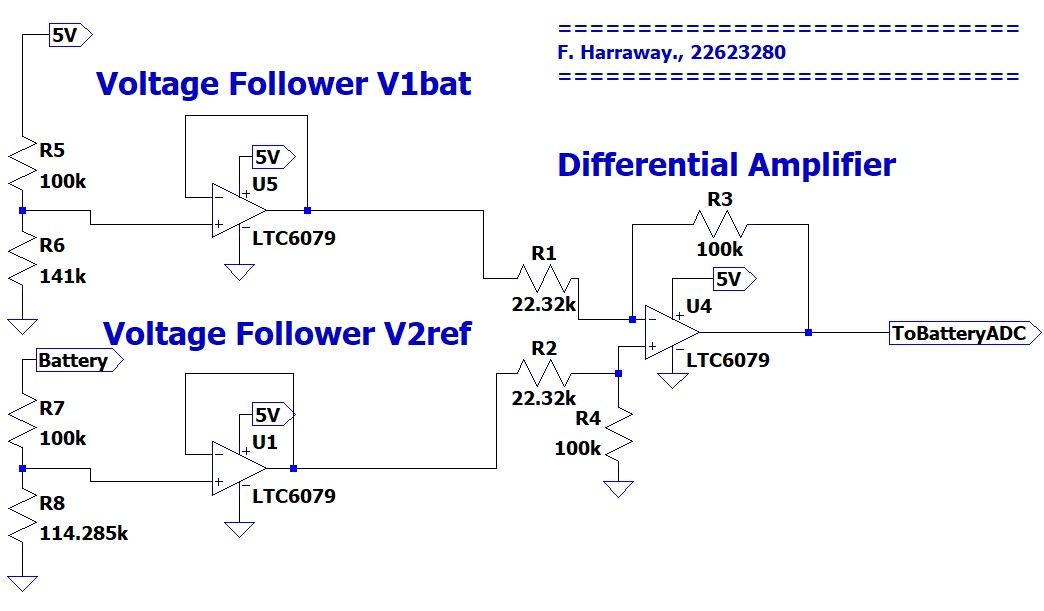
\includegraphics[width=0.5\linewidth]{Figures/A6/Batterysig.jpg}
	\caption{Battery measurement circuit}
	\label{fig:batcirc}
\end{figure}


\begin{table}[!htb]
	\centering
	\footnotesize
	\caption[Battery voltage measurement circuit op amp requirements]{Battery voltage measurement circuit op amp requirements \cite{MCP}}
	\begin{tabular}{lrrrr}
		\toprule
		& $Min$ &$Max$&$Designed$ $range / value$\\
		&[V]&[V]&[V]\\
		\midrule
		All op amps Difference between supply rails $V_{DD} - V_{SS}$ & -& 7  &5   \\
		
		U1 Common mode voltage $(\frac{V_+ + V_-}{2}-V_{SS})$ &  -0.3&5.3&3-4\\
		U1 Input voltages to $V_-$ and $V_+$  &  -1    &6& 3-4 \\
		
		U5 Common mode voltage $(\frac{V_+ + V_-}{2}-V_{SS})$ &  -0.3&5.3&2.92\\
		U5 Input voltages to $V_-$ and $V_+$ &  -1    &6& 3-4 \\
		
		
		U4 Common mode voltage $(\frac{V_+ + V_-}{2}-V_{SS})$ &  -0.3&5.3&2.48-3.28\\
		U4 Input voltages to $V_-$ and $V_+$  &  -1    &6&2.48-3.28 \\
		U4 Differential Voltage $ (|V_+ - V_-|)$ & -& 5&  3.28  \\
		
		\bottomrule
	\end{tabular}
	\label{tab:MCPbat}
\end{table}

From table \ref{tab:MCPbat}, all op amps are operating within working ranges.







%%%%%%%%%%%%%
\chapter{Subsystem results}\label{chap:res}
\section{Voltage regulation}
In the following graphs three different conditions will be setup to analyse the simulations performance. The three setups include having the supply powered on and then turning the NMOS off when it was initially on. The second setup is with the supply on and then turning the initially off NMOS, on. the last setup will be with the NMOS off and the supply off. In each of the setups the currents and voltages at the chosen nodes will be analysed.

\begin{figure}[!htb]
 \footnotesize
 \centering
    \begin{subfigure}[]{0.42\textwidth}
              \centering
  		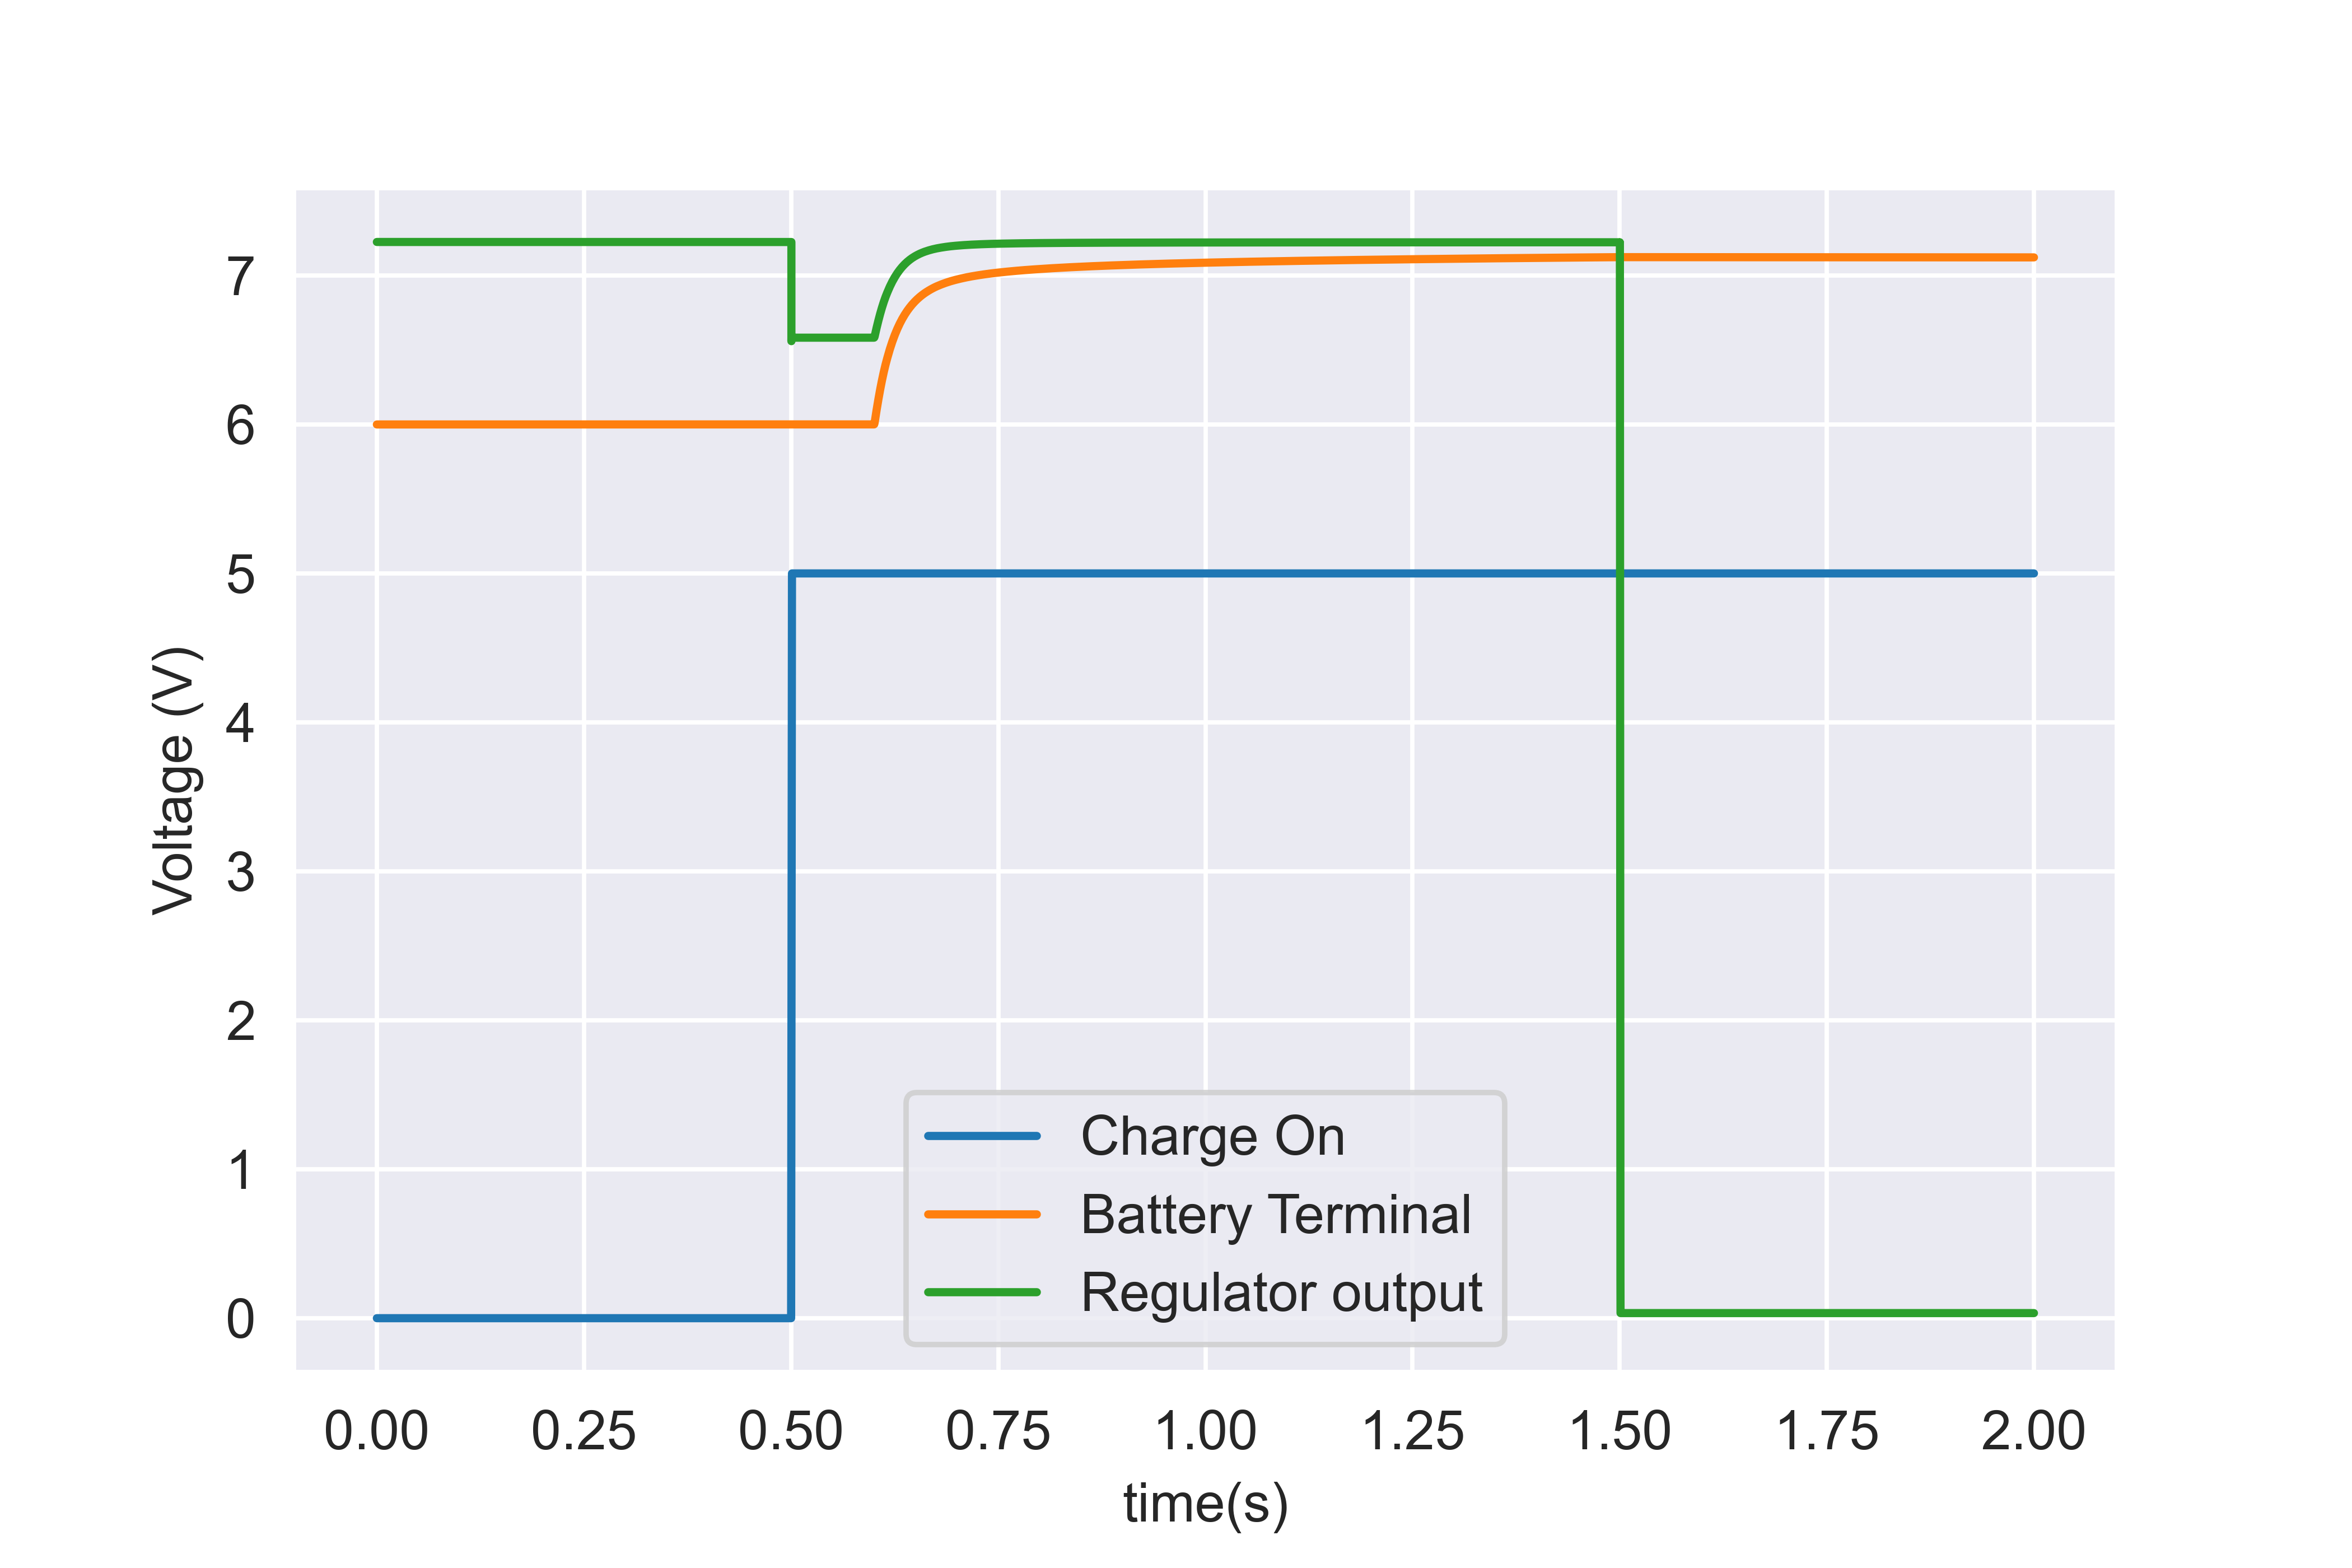
\includegraphics[width=1\linewidth]{./Figures/A2-1.png}
		    \caption{} \label{subfig:A2-1}
     \end{subfigure}
     \begin{subfigure}[]{0.42\textwidth}
             \centering
  		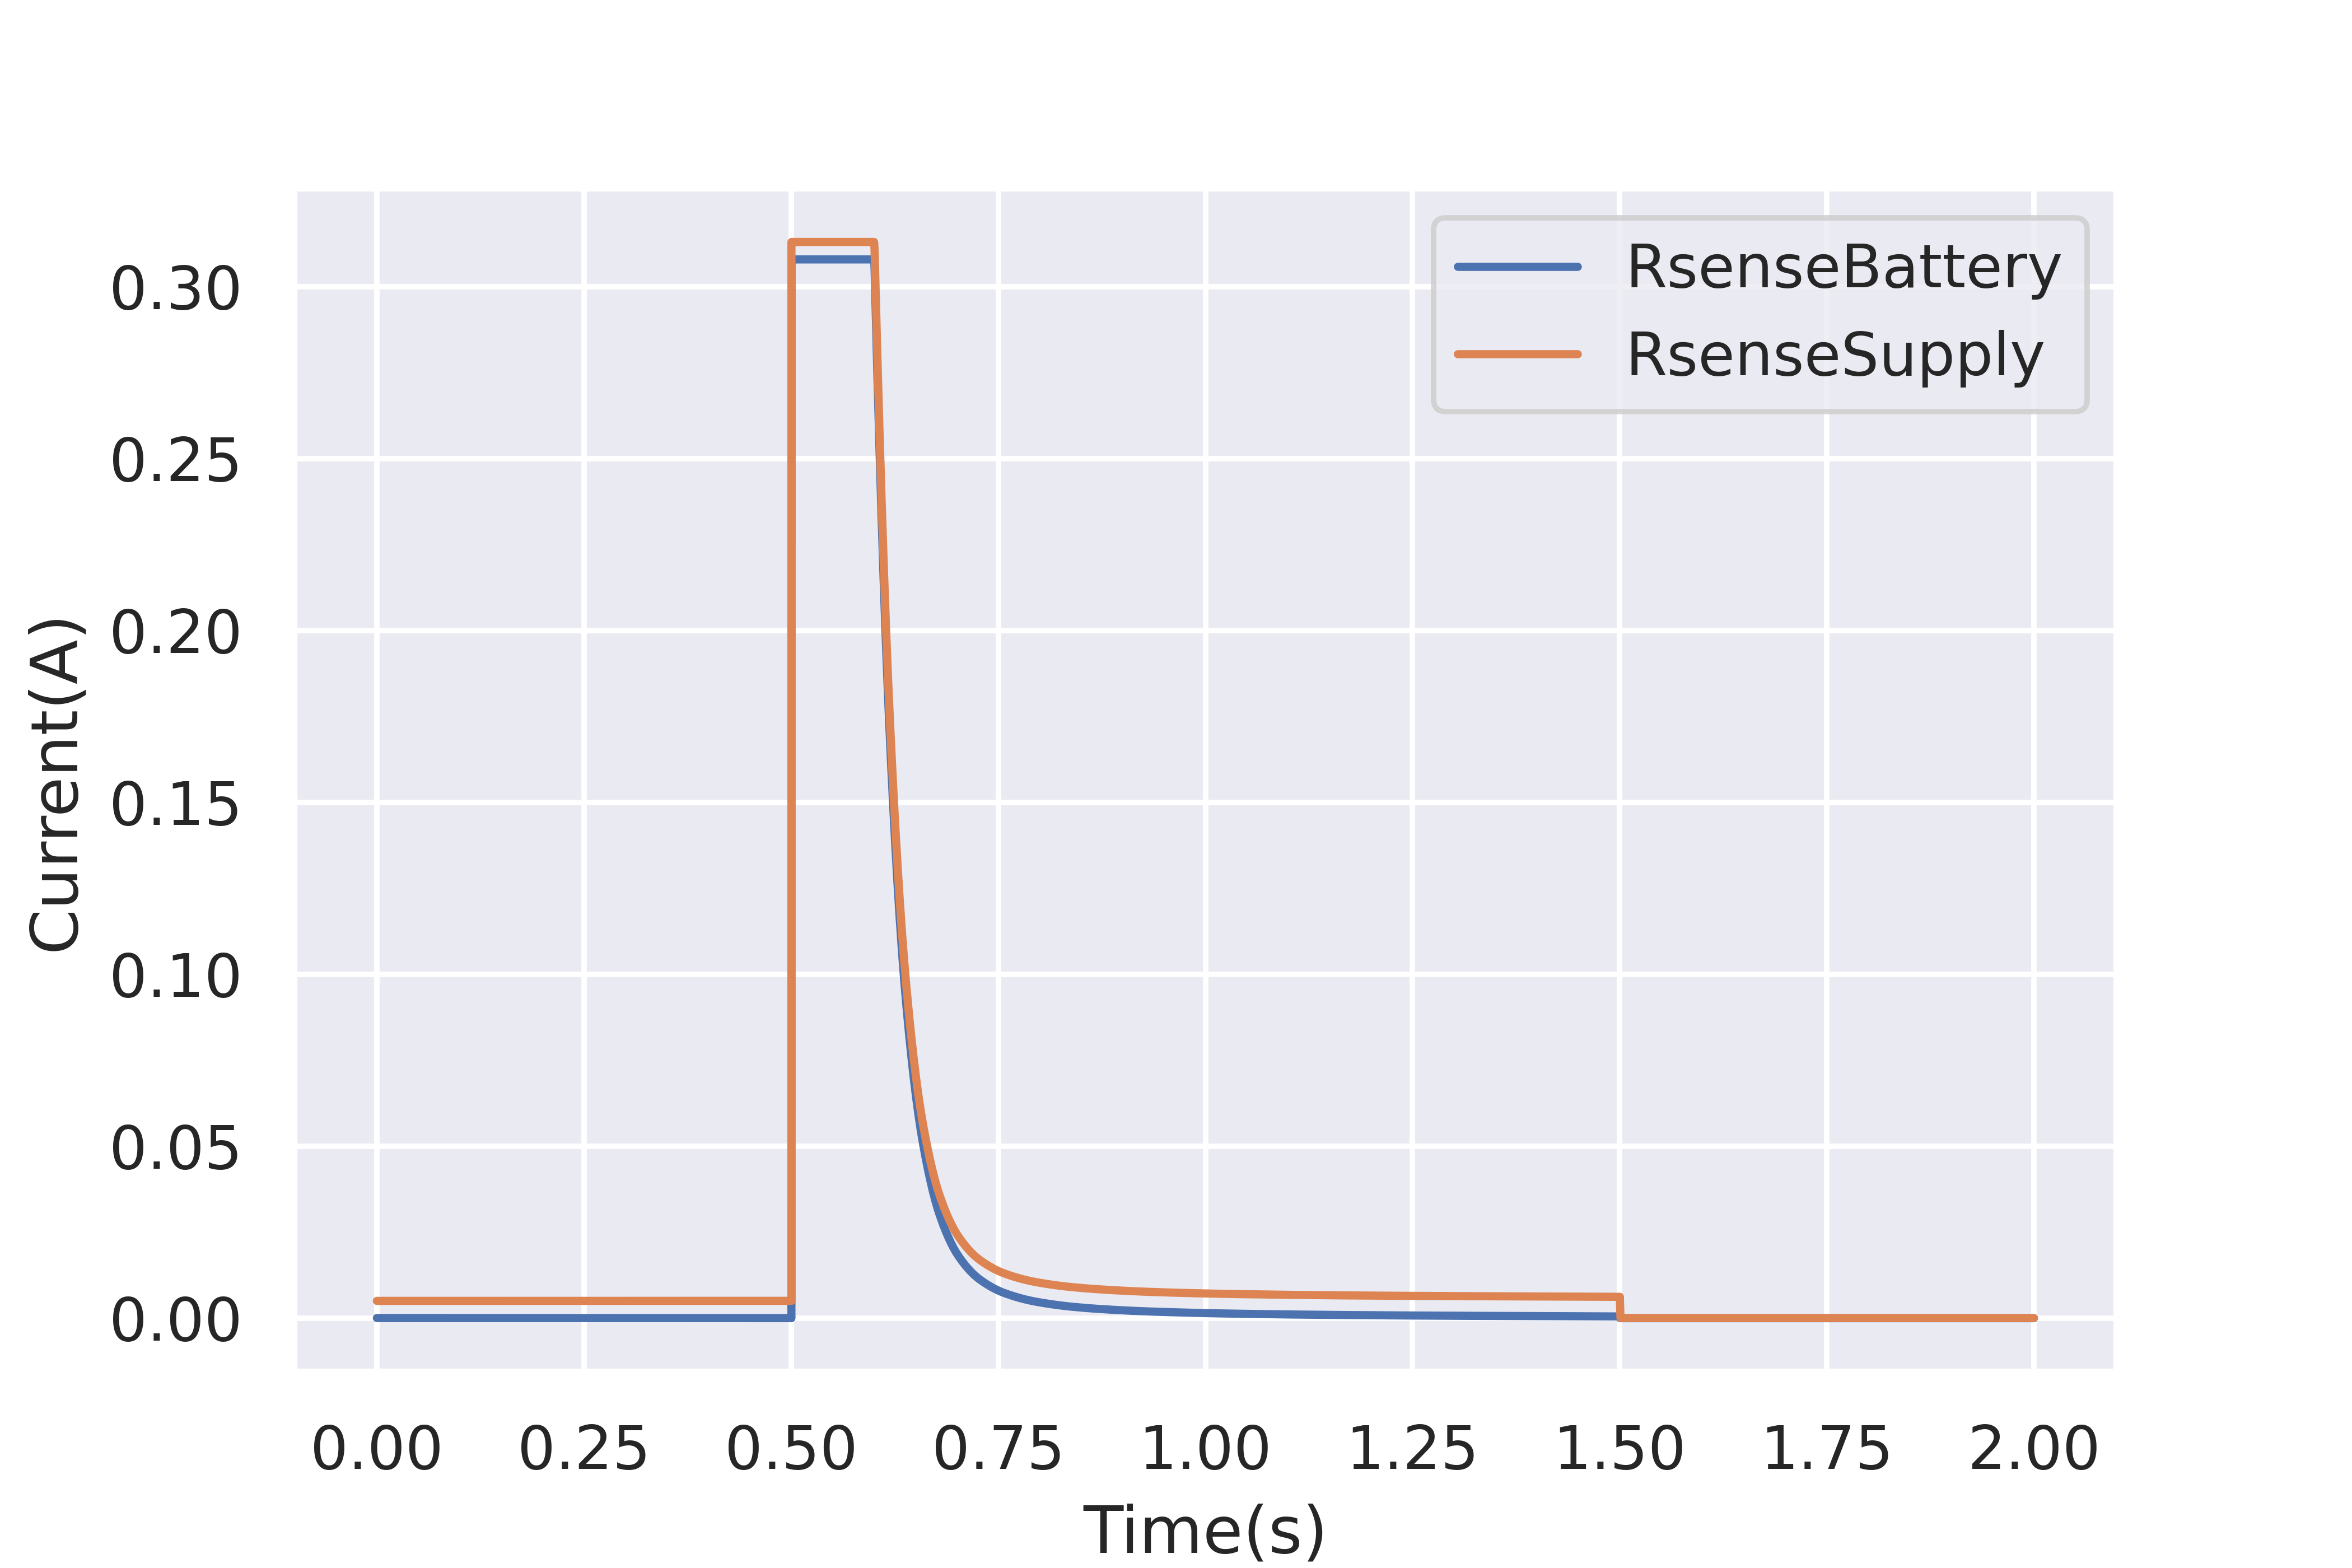
\includegraphics[width=1\linewidth]{./Figures/A2-2.png}
		   \caption{ } \label{subfig:A2-2}
     \end{subfigure}
   \caption[{LTSPICE switch turning on results}]{LTSpice Results for switch turning on  (a)  Relevant Voltages (b)  Relevant currents  }
    \label{fig:spiceReg}
 \end{figure}

 From figures \ref{subfig:A2-2} it can be seen that the maximum current flowing into the battery is just over 300mA. This current is much less than 1.2A and will therefore not damage the battery. The current only starts flowing when "charge on" (the control signal to the high side switch) goes high.
 
 \begin{figure}[!htb]
 \footnotesize
 \centering
    \begin{subfigure}[]{0.42\textwidth}
              \centering
  		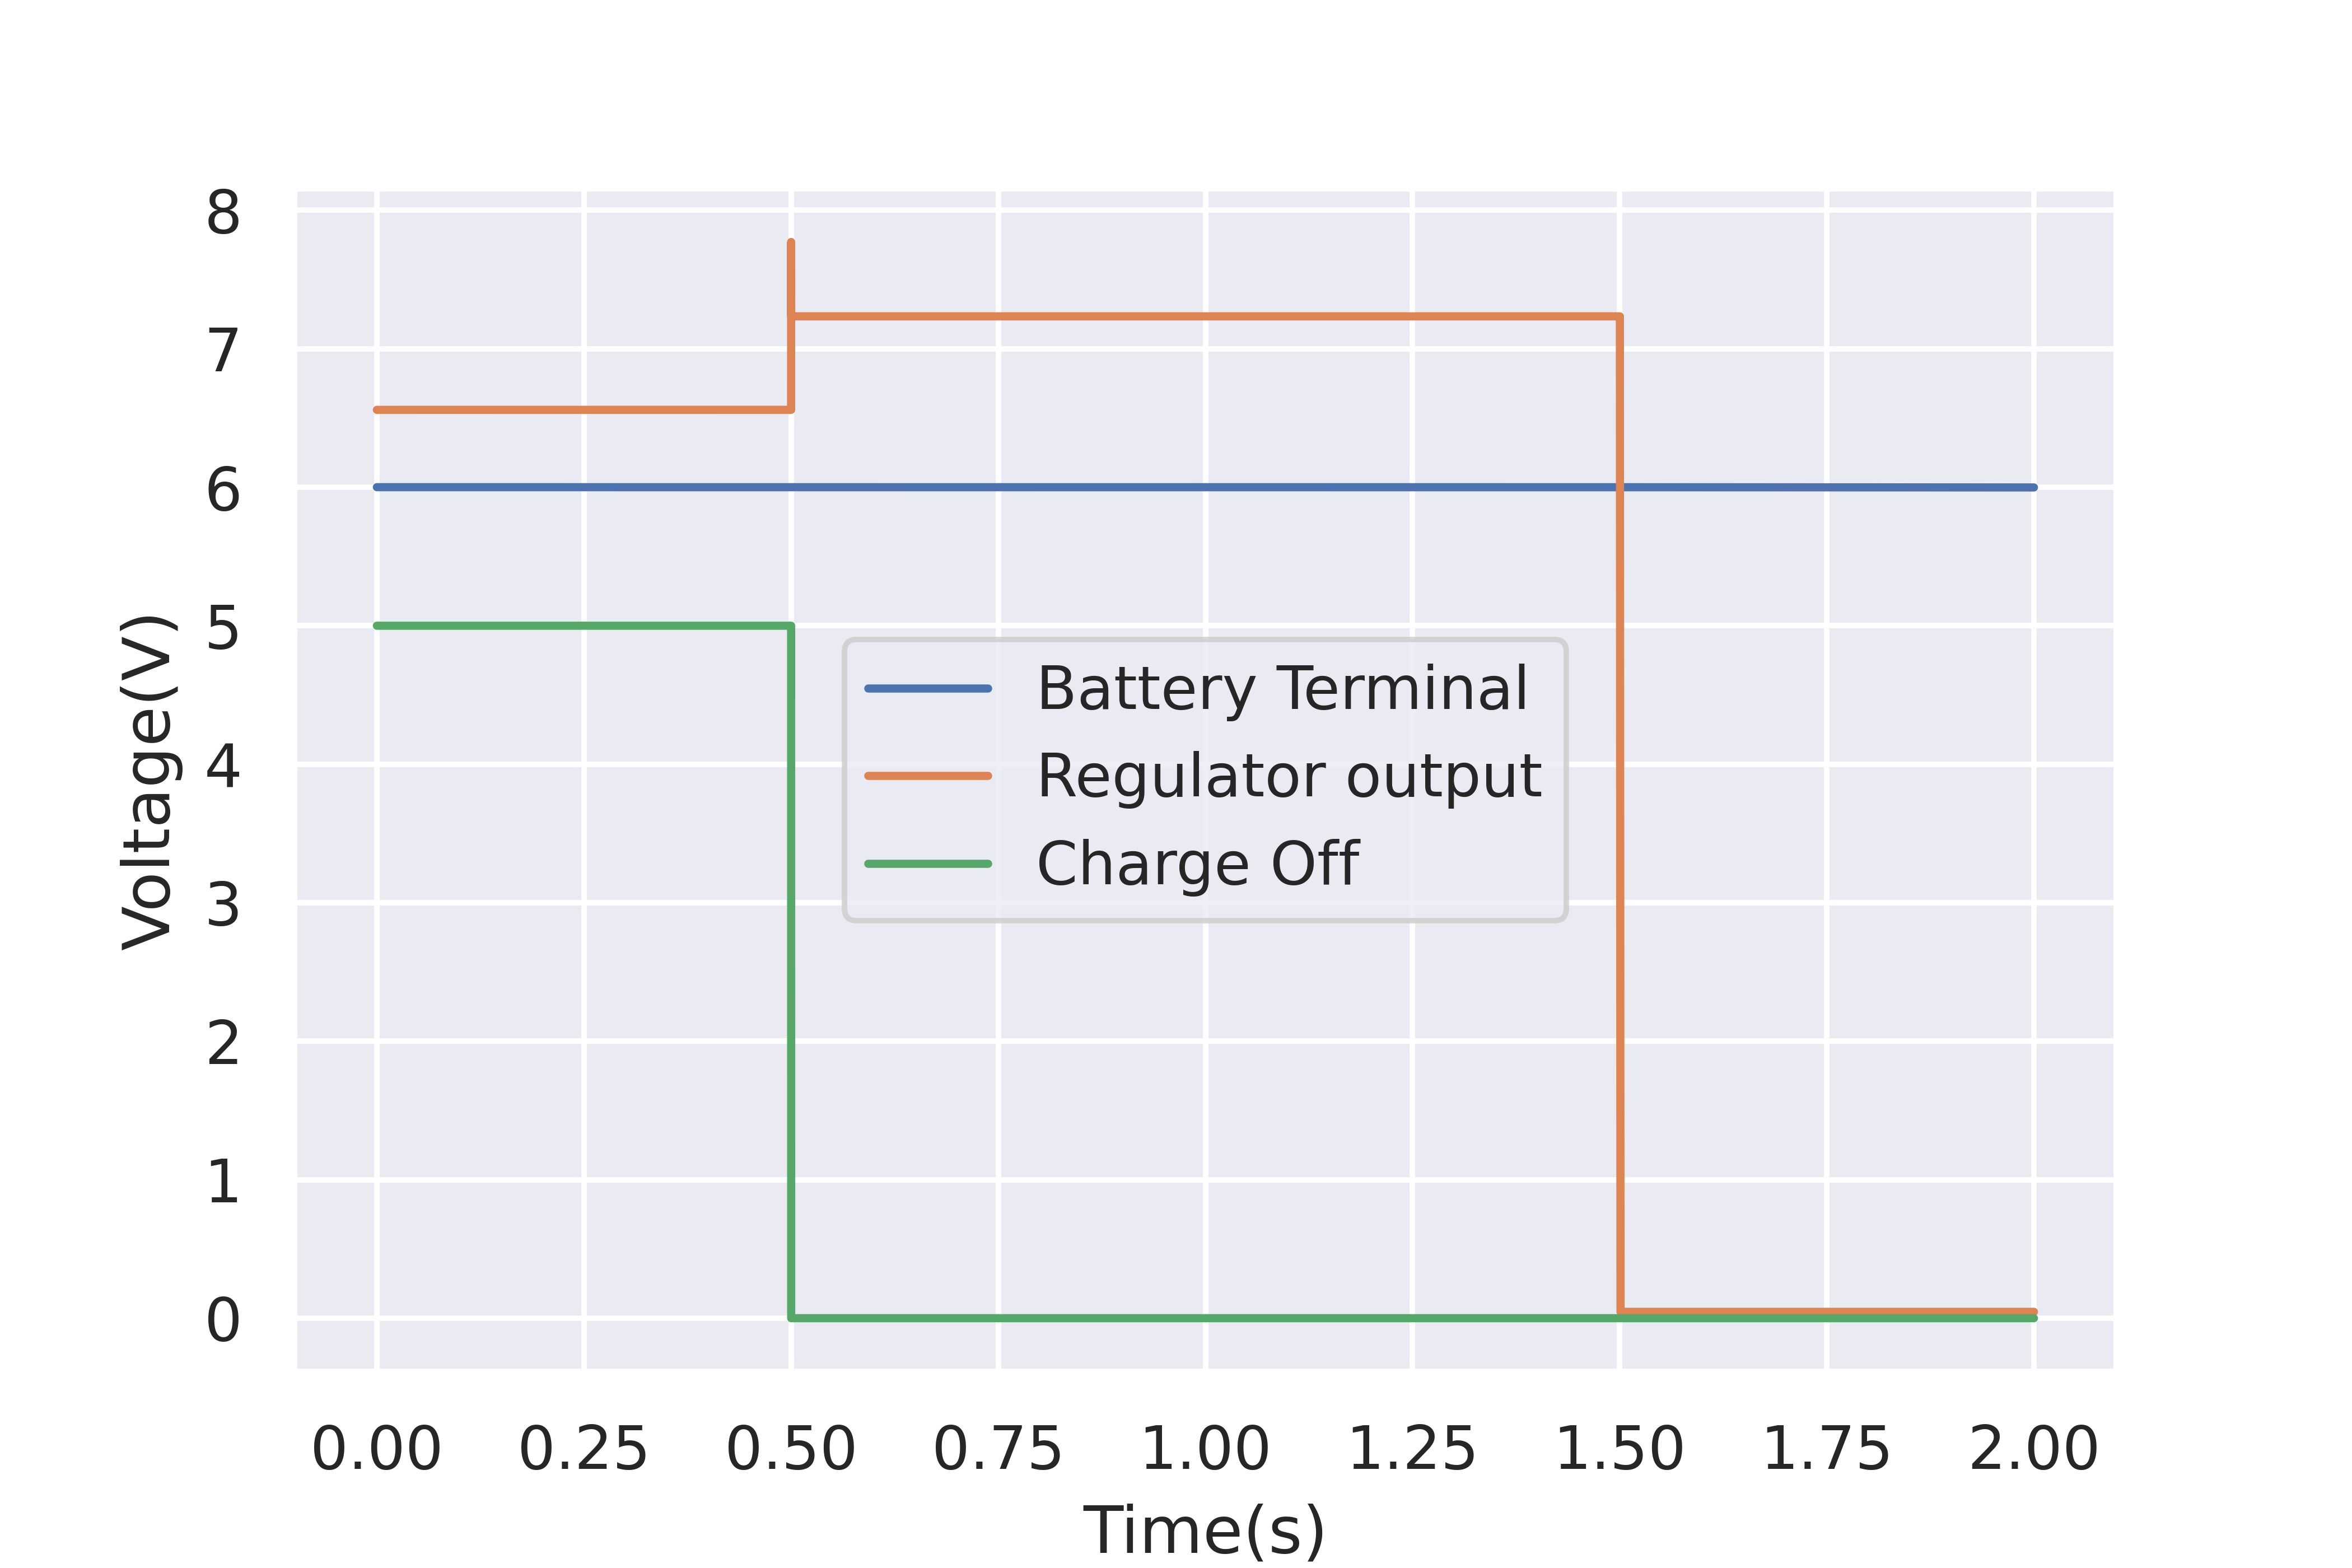
\includegraphics[width=1\linewidth]{./Figures/A2-3.png}
		    \caption{} \label{subfig:A2-3}
     \end{subfigure}
     \begin{subfigure}[]{0.42\textwidth}
             \centering
  		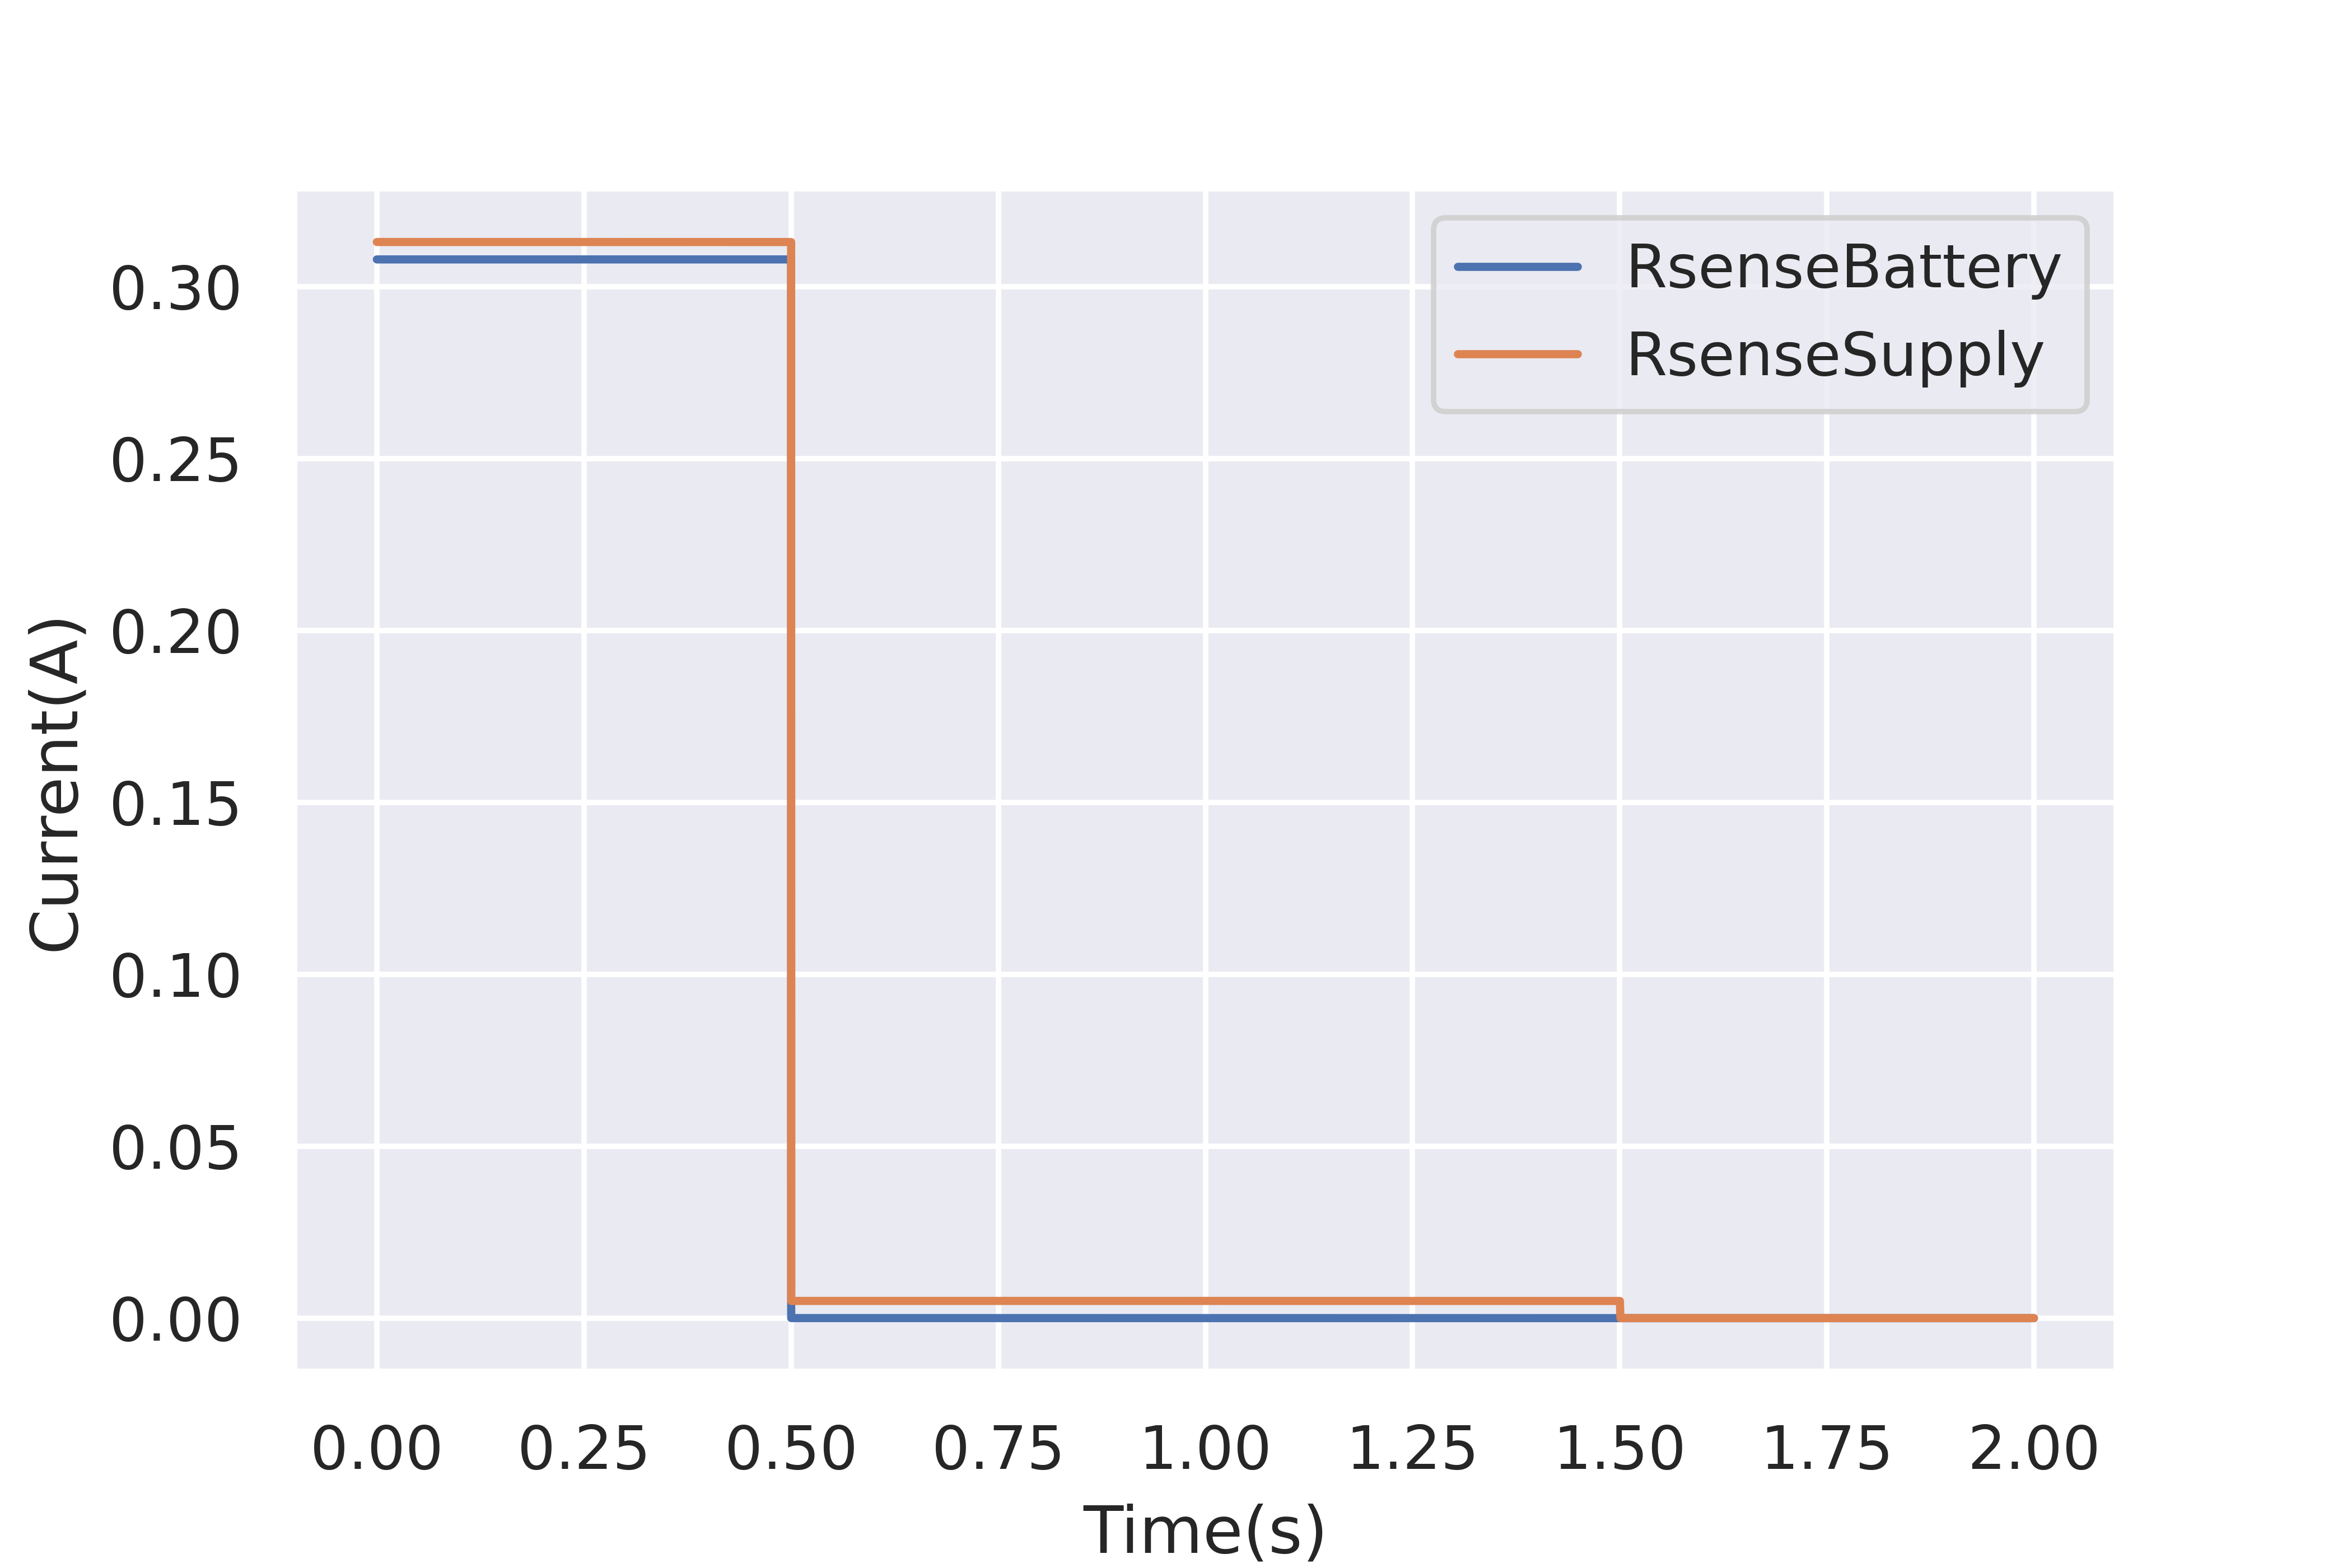
\includegraphics[width=1\linewidth]{./Figures/A2-4.png}
		   \caption{ } \label{subfig:A2-4}
     \end{subfigure}
   \caption[{LTSPICE switch turning off results}]{LTSpice Results for switch turning off  (a)  Relevant Voltages (b)  Relevant currents  }
    \label{fig:two}
 \end{figure}
 \newpage
 In figure \ref{fig:two} it can be seen that as soon as Charge Off goes low (NMOS turns off) the current to the battery stops flowing and the battery voltage remains at 6V.



 \begin{figure}[!htb]
 \footnotesize
 \centering
    \begin{subfigure}[]{0.42\textwidth}
              \centering
  		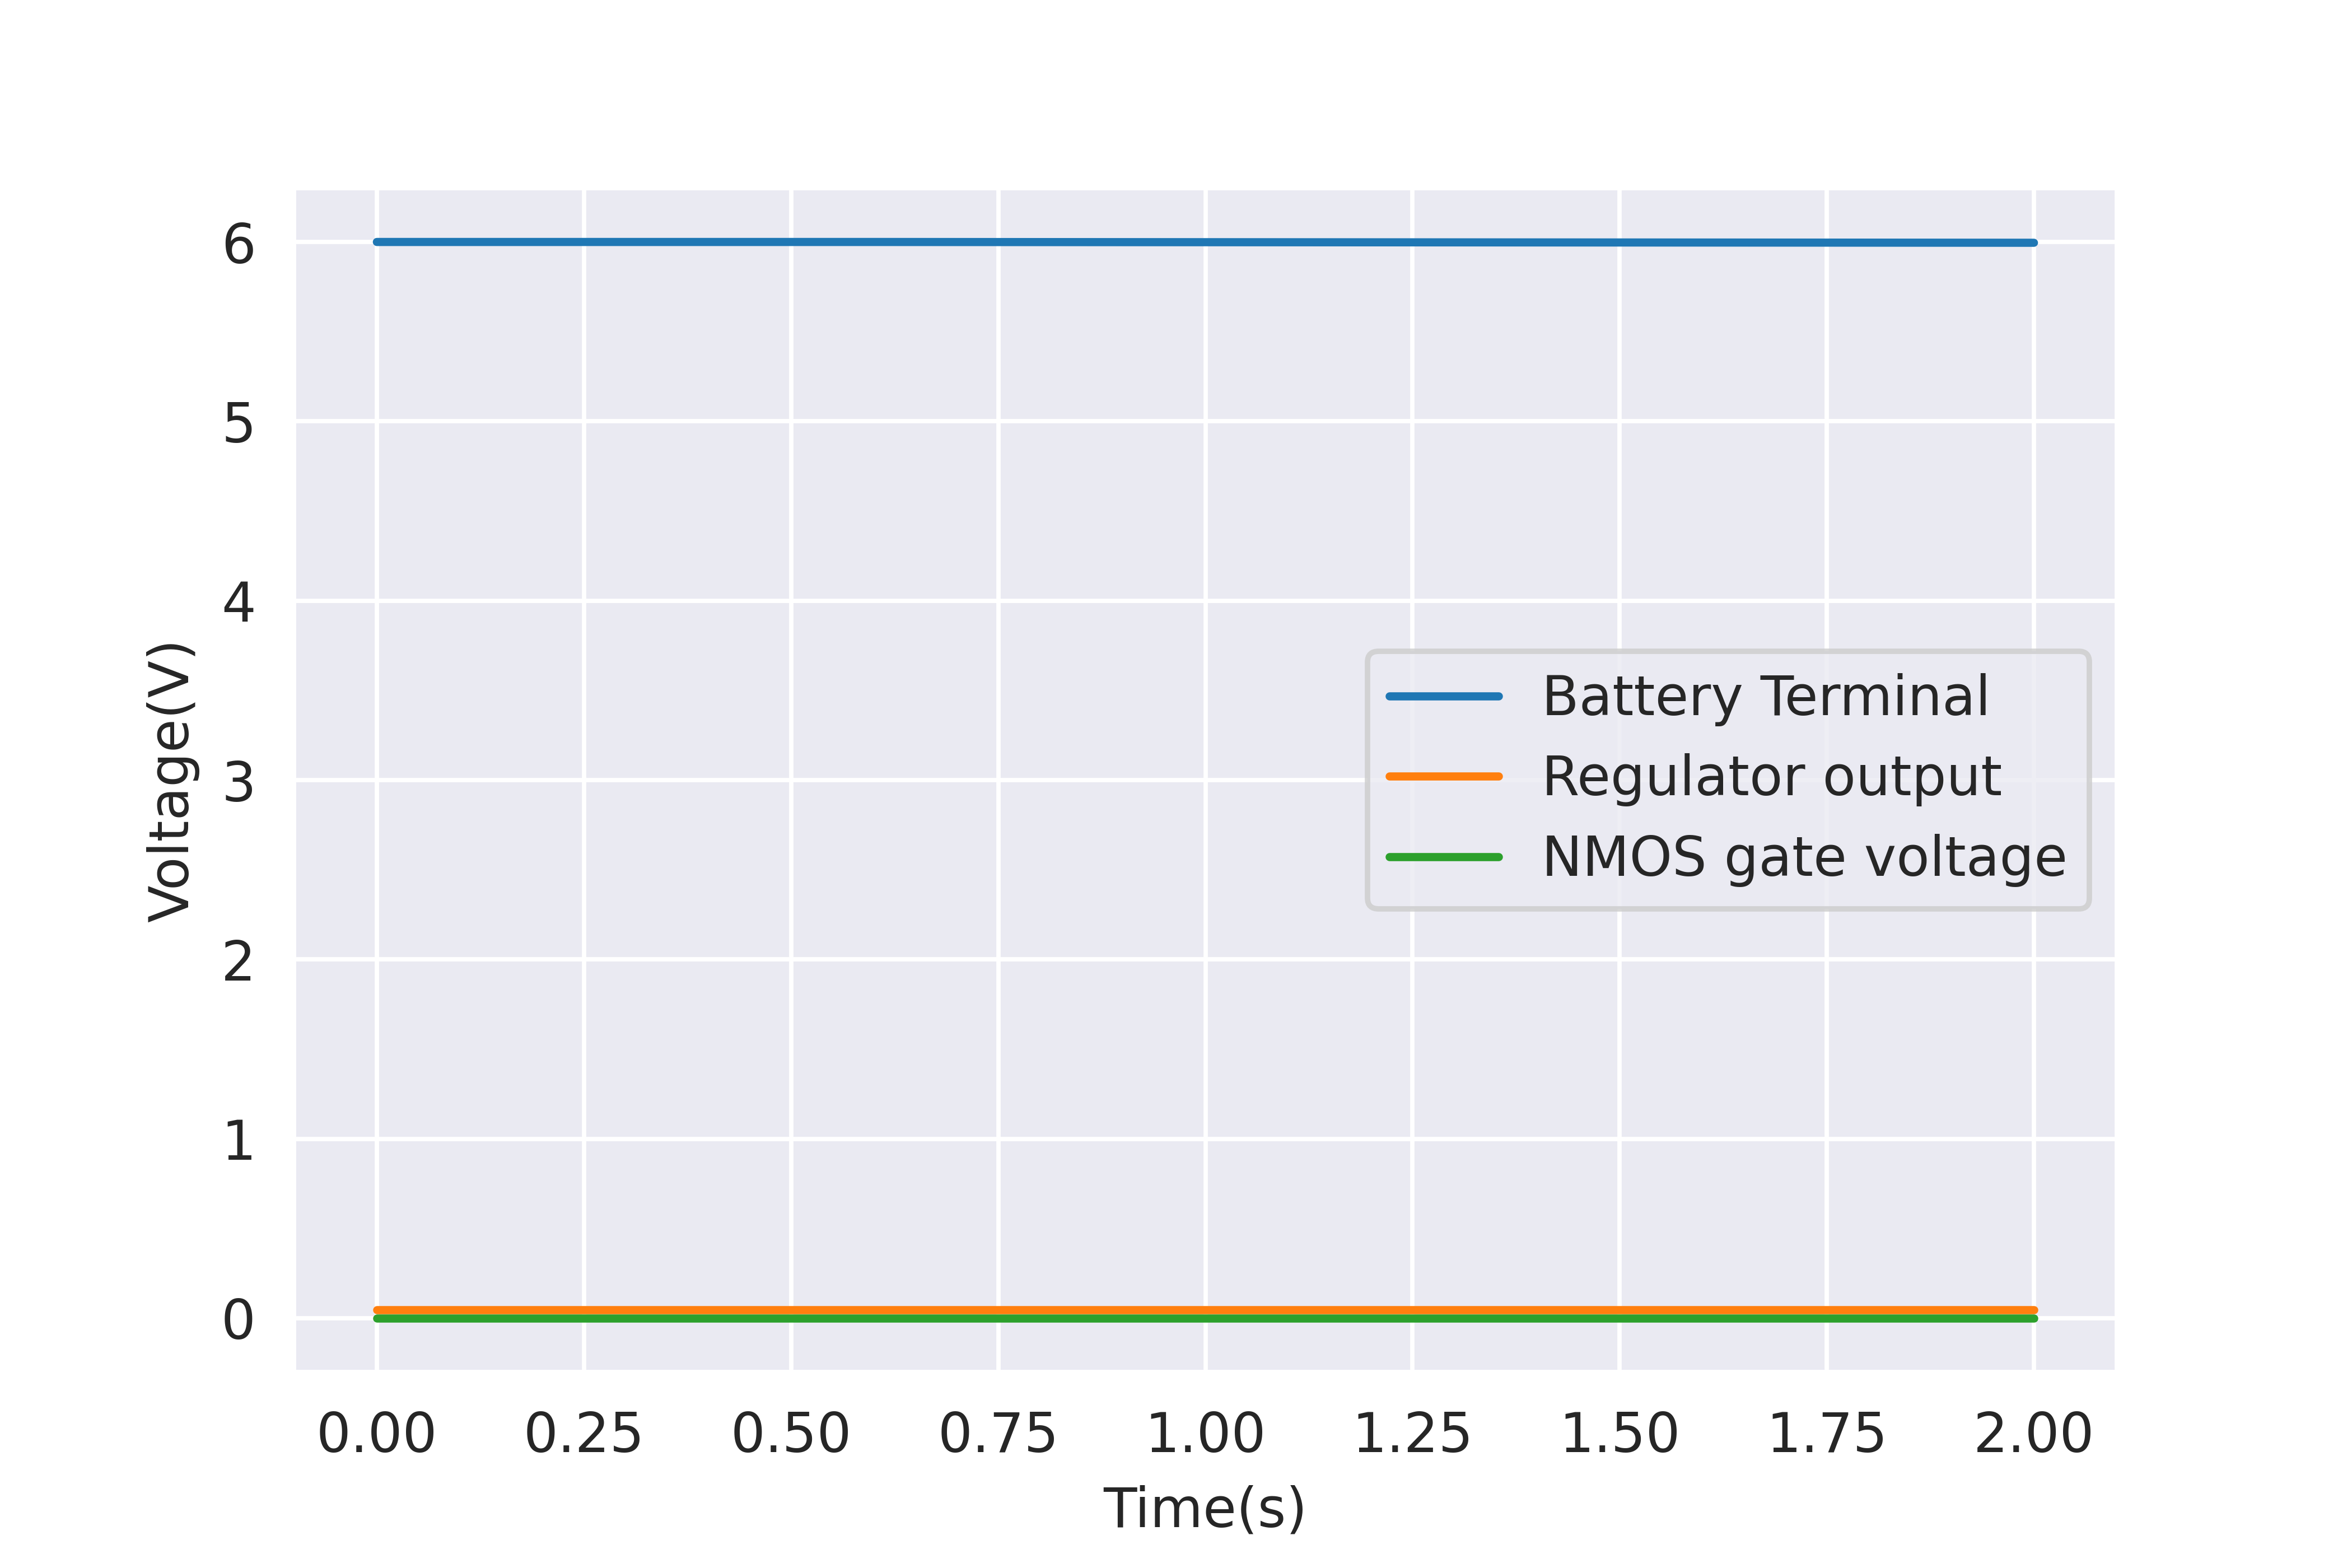
\includegraphics[width=1\linewidth]{./Figures/A2-5.png}
		    \caption{} \label{subfig:A2-5}
     \end{subfigure}
     \begin{subfigure}[]{0.42\textwidth}
             \centering
  		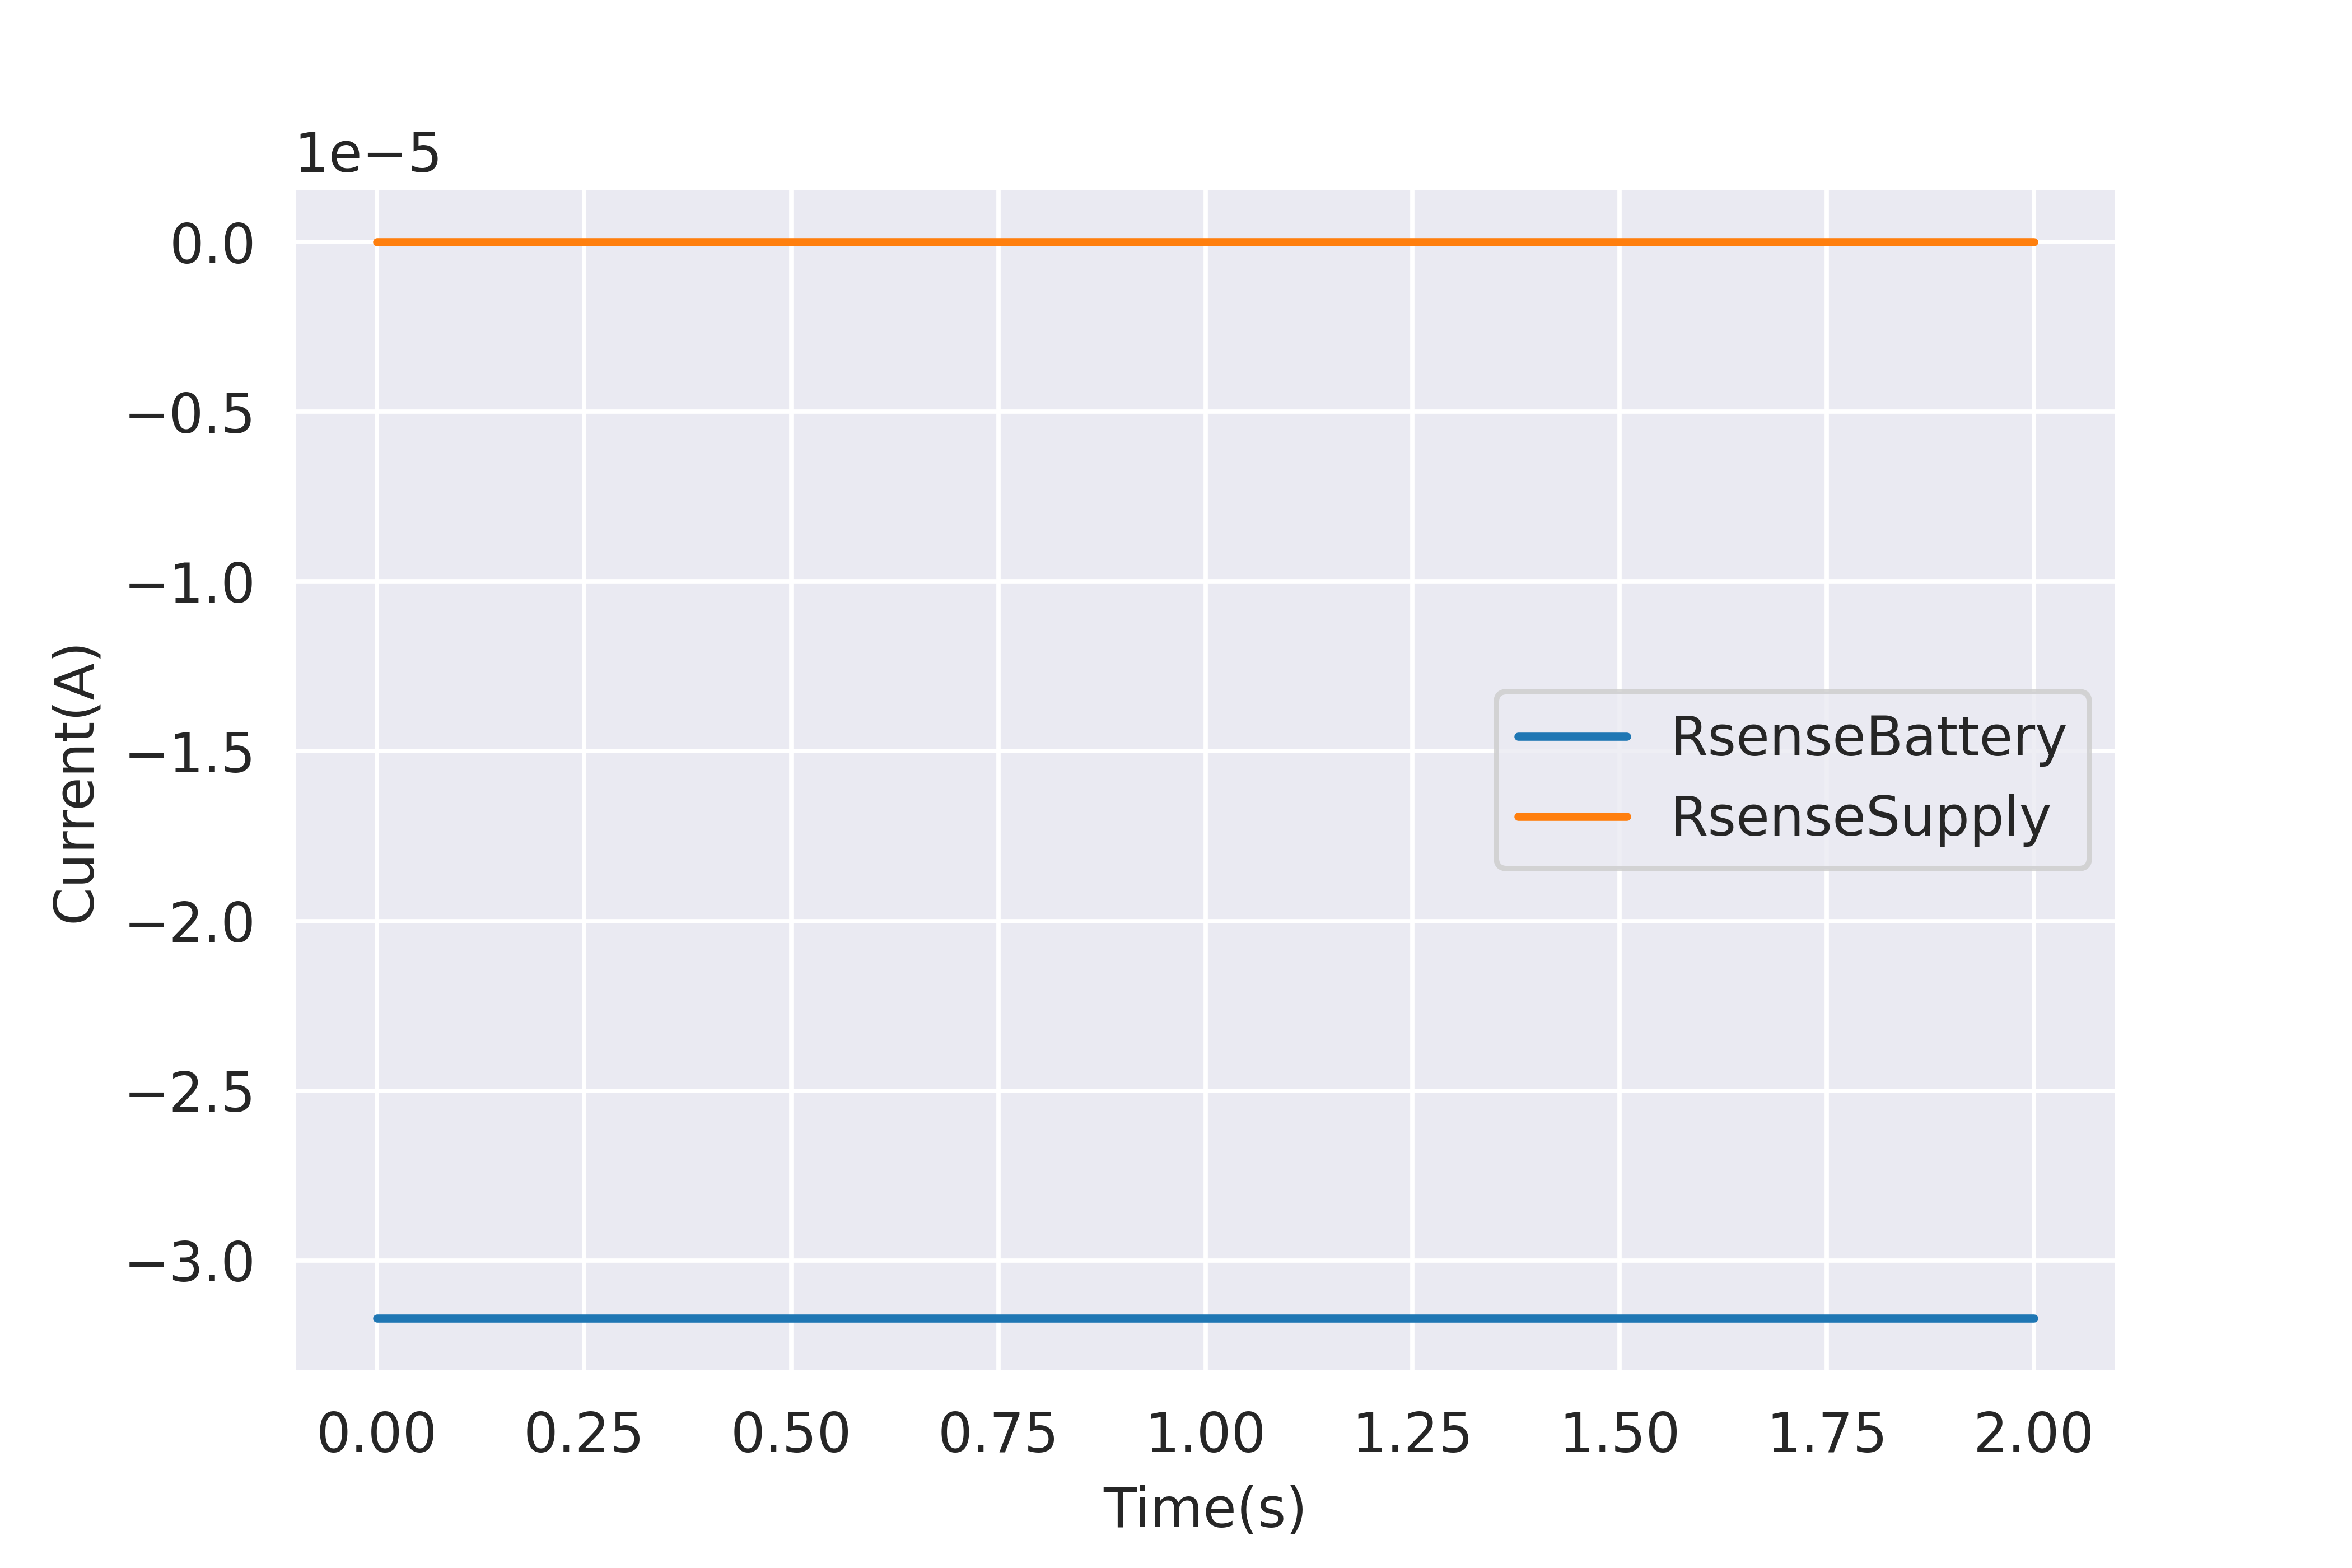
\includegraphics[width=1\linewidth]{./Figures/A2-6.png}
		   \caption{ } \label{subfig:A2-6}
     \end{subfigure}
   \caption[{LTSPICE switch off and supply off results}]{LTSpice Results for supply off and NMOS gate pulled low  (a)  Relevant Voltages (b)  Relevant currents  }
    \label{fig:three}
 \end{figure}
In figure \ref{fig:three} both the supply and the switch are off. This then shows the discharge current of just above 30\textmu A. It is small enough that I would say specifications are met.


%**********************************************

\begin{table}[!htb]
        \centering
        \footnotesize
        \caption{Measured Values}
         \begin{tabular}{lrrrr}
          \toprule
             & Voltage at battery connection terminal \\
             &  [V] \\
          \midrule
          Open Circuit & 7.27     \\
          1K Load &  7.1     \\
          10K load &  7.0     \\

          \bottomrule
        \end{tabular}
     \label{tab:regmeas}
\end{table}
From table \ref{tab:regmeas} it can be seen that voltage is operating in the correct region of less than 7.2V. More results regarding the charging can be found in section \ref{sec:sysRes} in table \ref{tab:batsys}.



 

%**********************************************
%%%%%%%%%%%%%%%%%%%%%%%%%%%%%%%%%%%%%%%%%%%%%%%%%
\newpage
\section{High side switch on supply side}

\begin{figure}[!htb]
 \footnotesize
 \centering
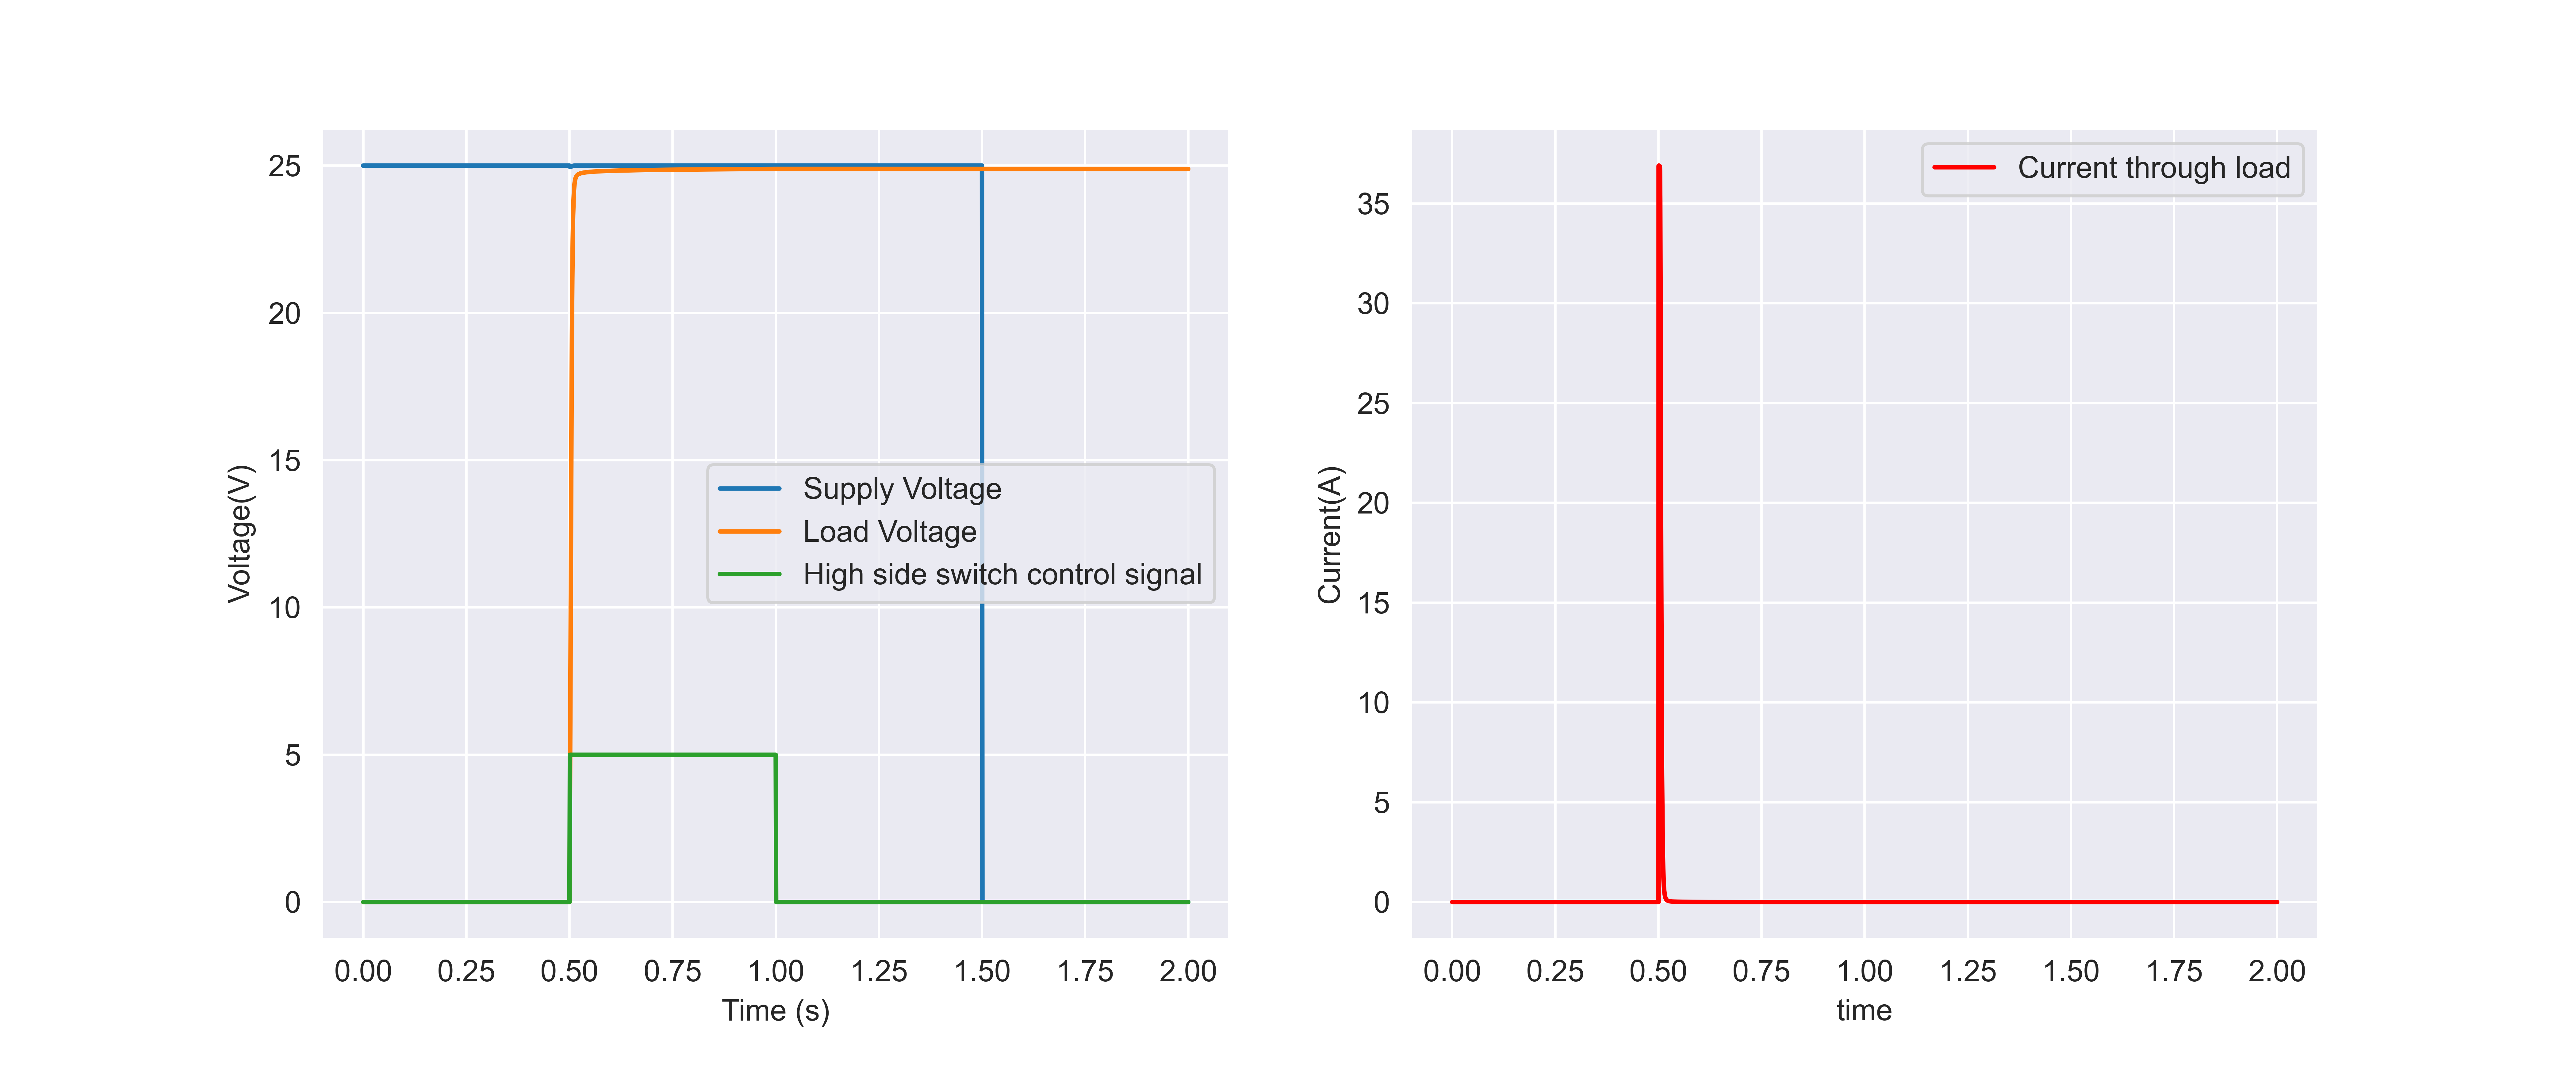
\includegraphics[width=0.8\textwidth]{Figures/A1.png}
\caption{LTSpice simulation results for high side switch on the supply side}
\label{fig:high-res}
 \end{figure}
 
 From figure \ref{fig:high-res} it can be seen that as soon as the high side witch control signal goes high, the load voltage changes to approximately the supply voltage. The current spikes as seen because the capacitor at the load charges up to the supply voltage very quickly.

\begin{table}[!htb]
        \centering
        \footnotesize
        \caption{Highside switch measurements}
         \begin{tabular}{lrrrr}
          \toprule
             & voltage from source to gate of the PMOS \\
             &  [V] \\
          \midrule
          Control signal at NMOS gate high &     6.94\\
          Control signal at NMOS gate low  &   0\\
         

          \bottomrule
        \end{tabular}
     \label{tab:PMOSmeas}
\end{table}
From the values in table \ref{tab:PMOSmeas} it can be seen that when the NMOS gate voltage goes high a voltage above the threshold voltage of the PMOS is applied, thus turning the switch on. For additional proof that the switch works, refer to figure \ref{fig:meas} where this switch successfully controlled the switching on and off of the charging circuit.
%%%%%%%%%%%%%%%%%%%%%%%%%%%%%%%%%%%%%%%%%%%%%%%%%
\newpage
\section{Undervoltage protection}
\begin{figure}[!htb]
 \footnotesize
 \centering
    \begin{subfigure}[]{0.45\textwidth}
              \centering
  		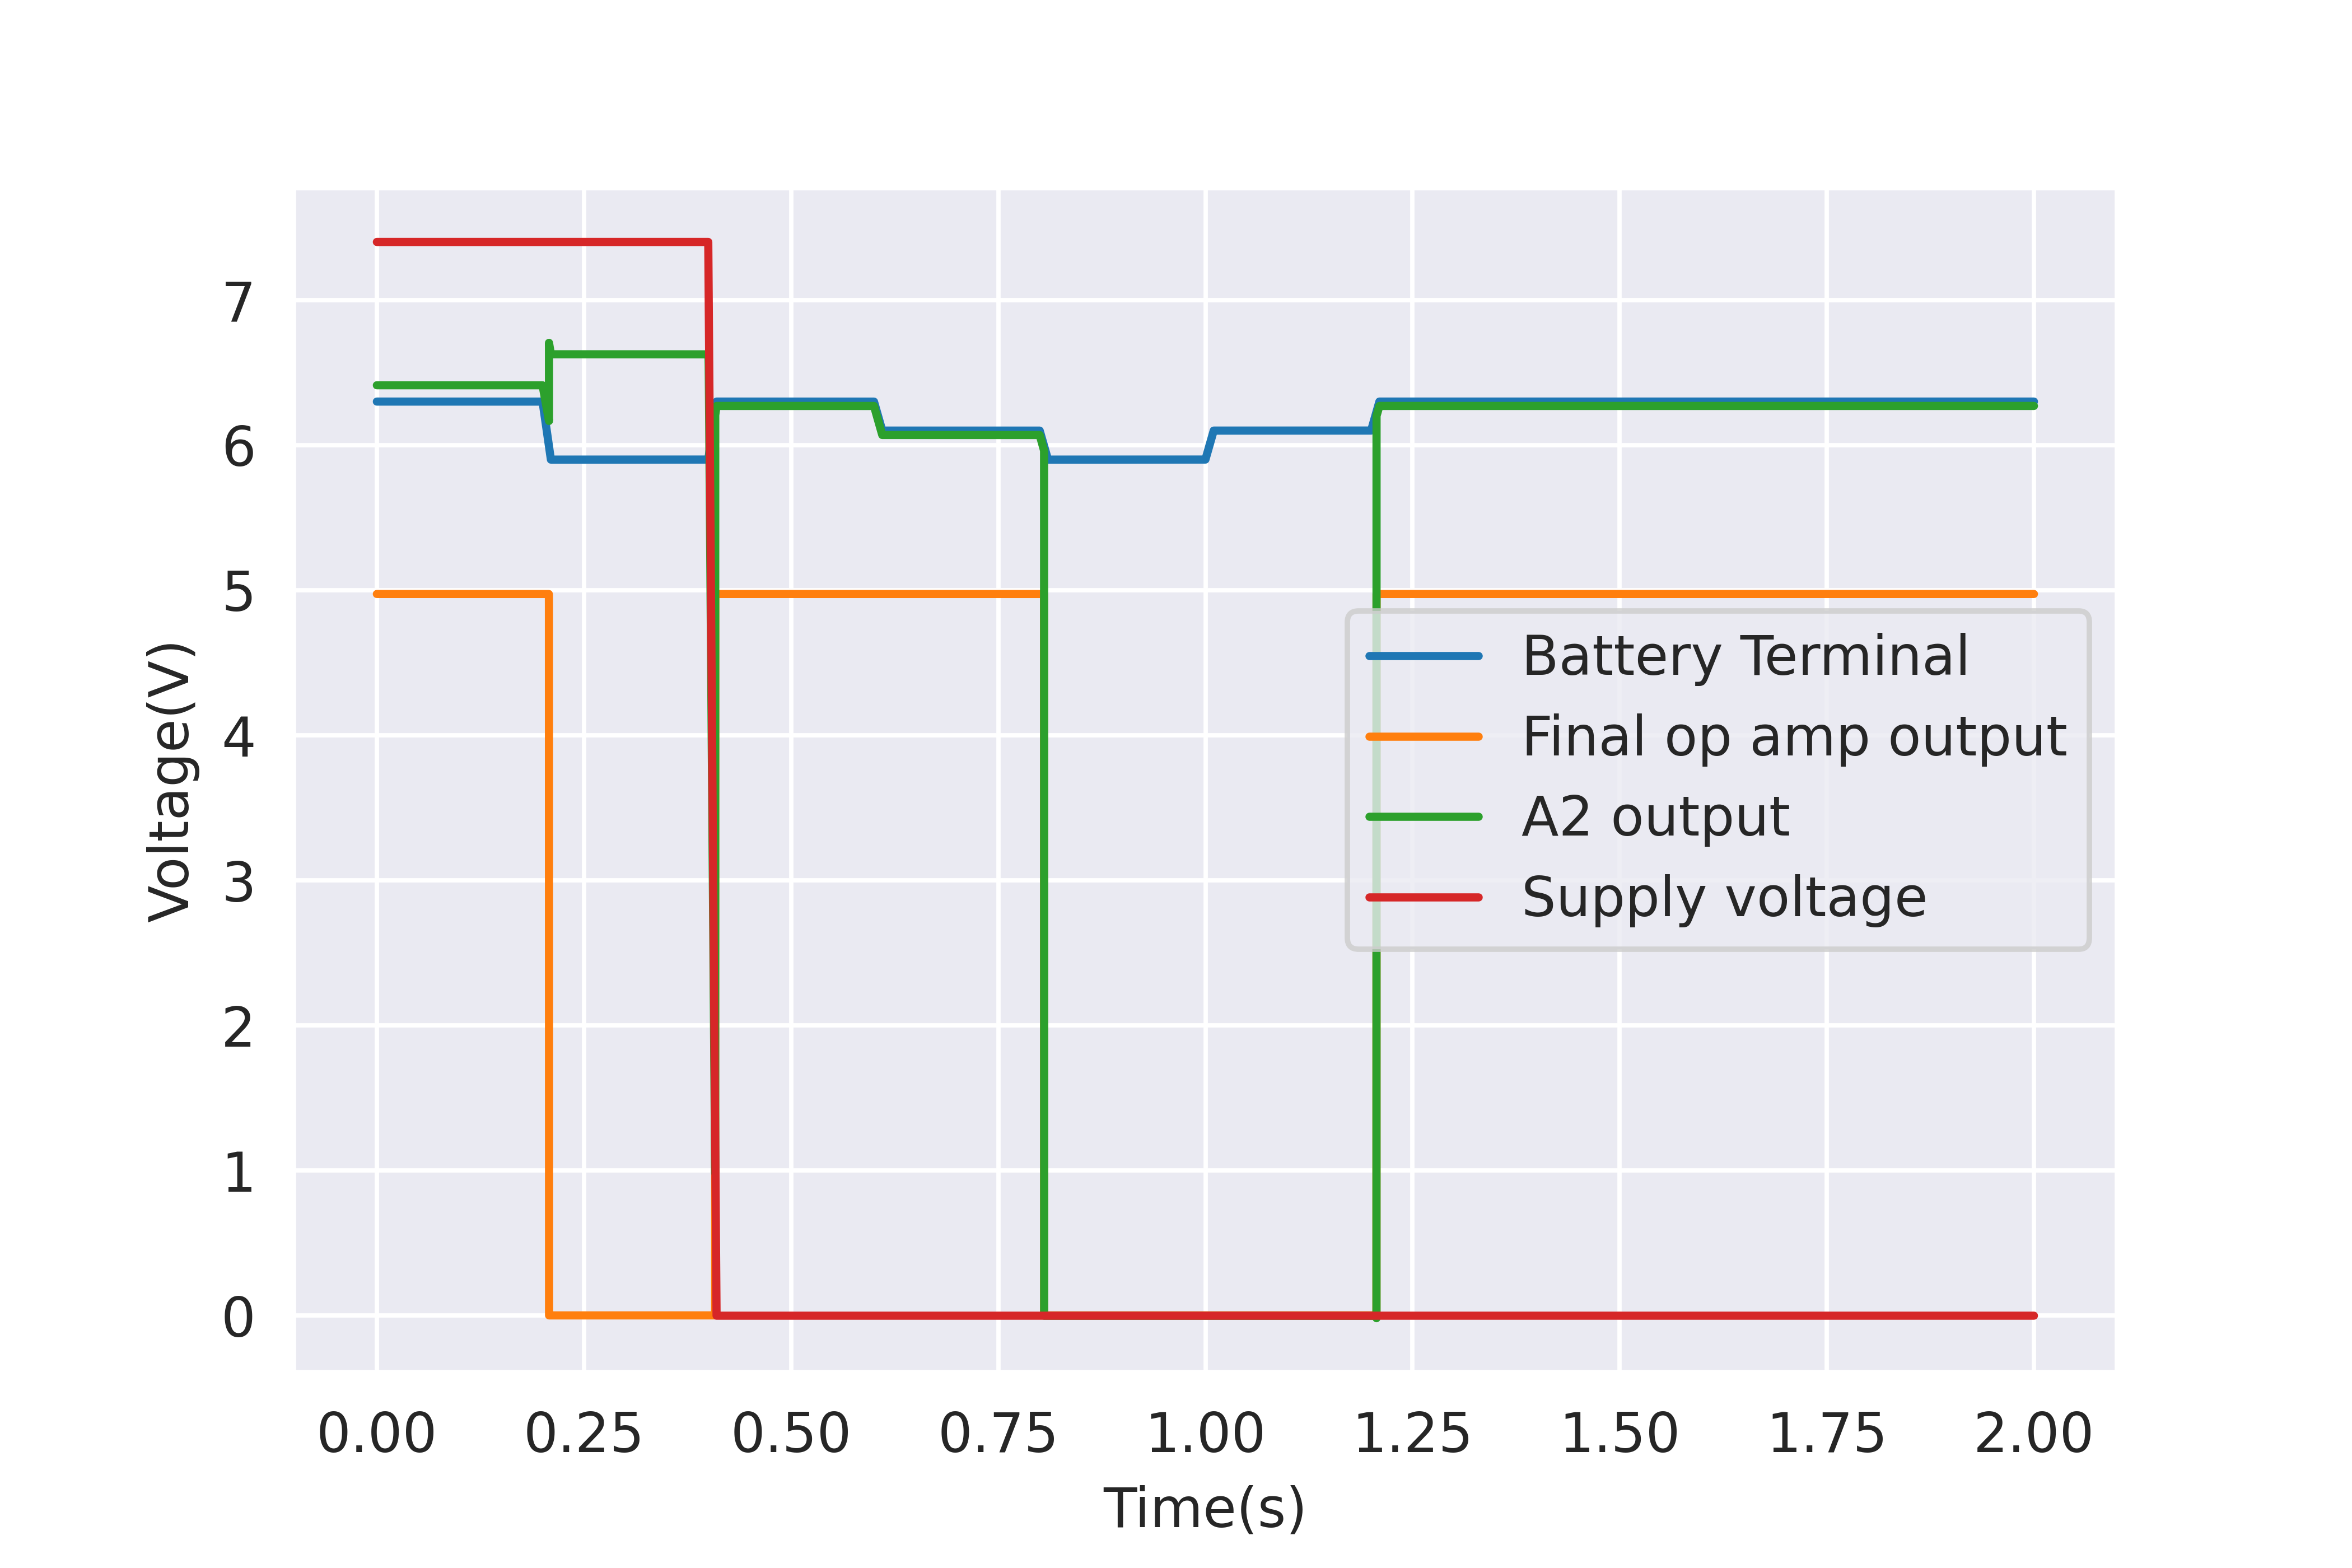
\includegraphics[width=1\linewidth]{./Figures/A31.png}
		    \caption{} \label{subfig:voltage}
     \end{subfigure}
     \begin{subfigure}[]{0.45\textwidth}
             \centering
  		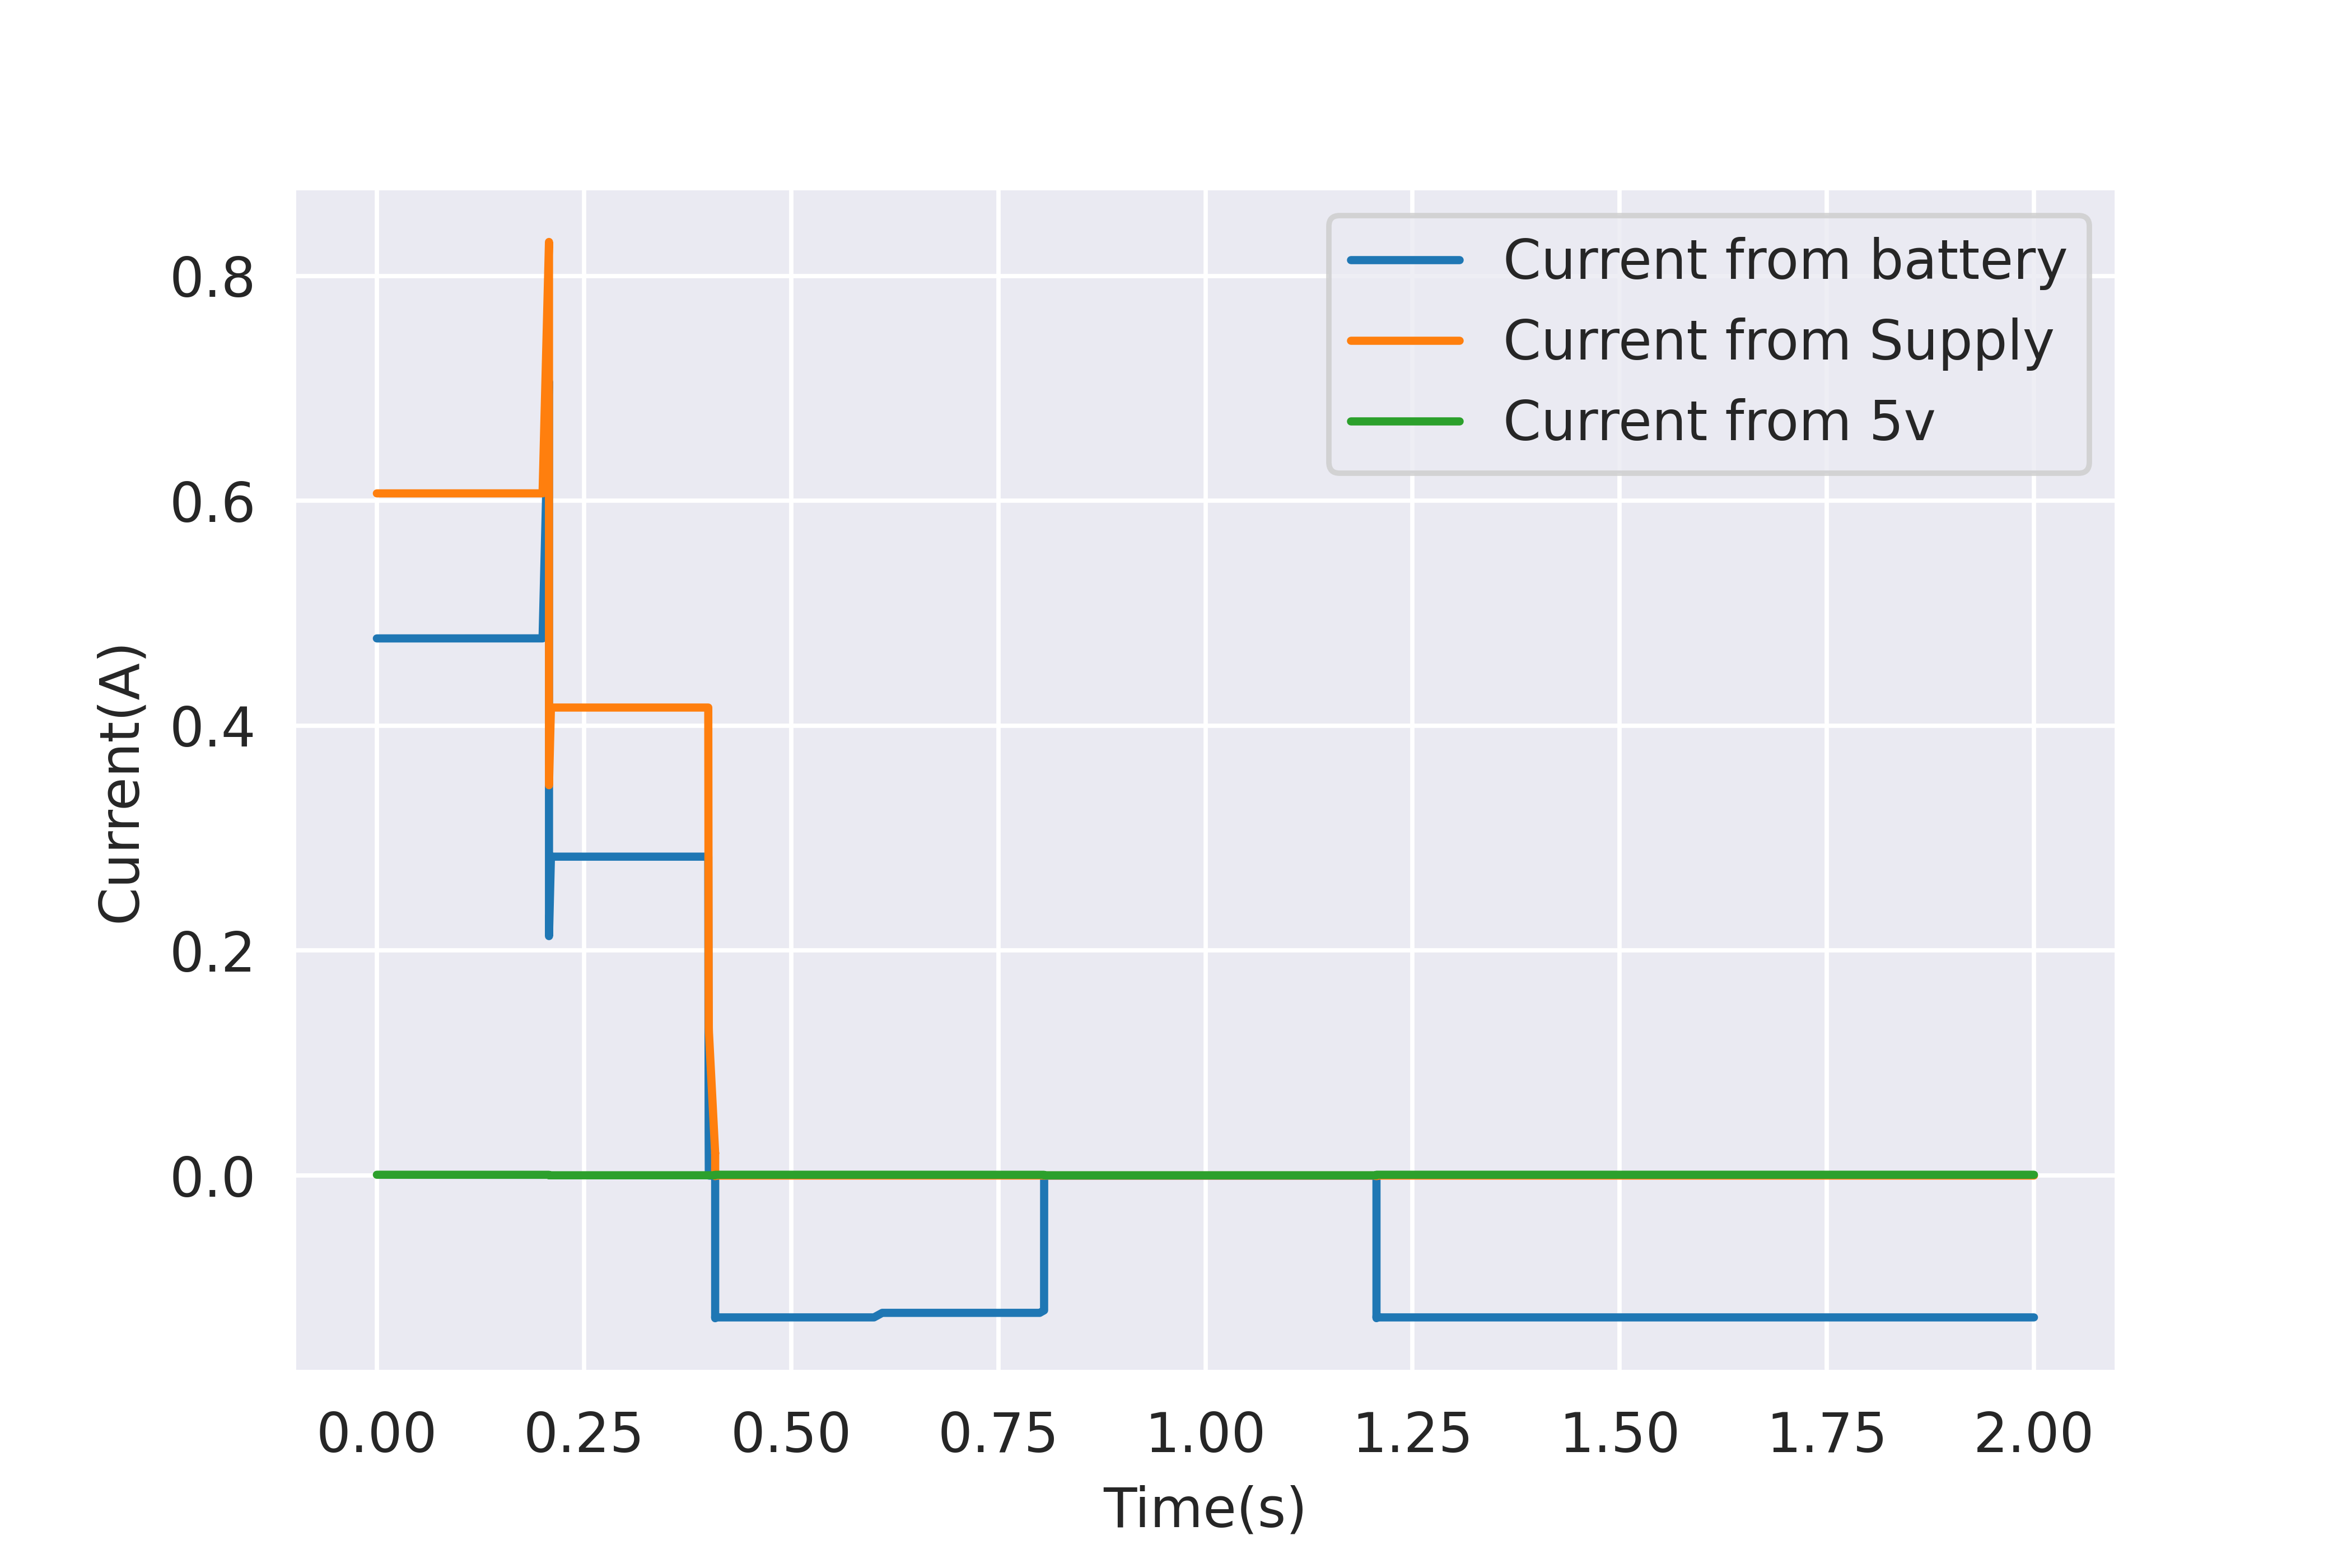
\includegraphics[width=1\linewidth]{./Figures/A32.png}
		   \caption{ } \label{subfig:current}
     \end{subfigure}
   \caption[{LT spice Results}]{LT spice results   (a) Relevant Voltages (b)  Relevant Currents }
    \label{fig:lt}
 \end{figure}


From figure \ref{subfig:voltage} it can be seen that the op amp transitions at the correct of 6V and 6.2V respectively. From figure \ref{subfig:current} it can be seen that the current out of the 5V regulator is less than 10mA and that the op amp output corresponds to the discharging from the battery. 



\begin{table}[!htb]
	\centering
	\footnotesize
	\caption{Under voltage circuit measurements}
	\begin{tabular}{lrrrr}
		\toprule
		& A2 Output& Battery terminal voltage \\
		&  [V]&[V] \\
		\midrule
		Stage 1 & 6.52 &6.48    \\
		Stage 2 &  5.98&0.14     \\
		Stage 3 &  6.20&0.13     \\
		Stage 4 &  6.40&6.33     \\
		
		\bottomrule
	\end{tabular}
	\label{tab:stagemeas}
\end{table}

\begin{flushleft}
\textbf{Stage 1}: Battery voltage is above 6V threshold and A2 output allows discharge.\newline
\textbf{Stage 2}: Battery voltage is below above 6V threshold and A2 output is 0V stopping battery discharge.\newline
\textbf{Stage 3}: Battery voltage is above 6V but not 6.2V (after under-voltage circuit disconnected battery) therefore A2 output is 0V, stopping battery discharge.\newline
\textbf{Stage 4}: Battery voltage is above 6.2V threshold after under-voltage circuit disconnected battery, therefore A2 is approximately equal to the battery voltage and is discharging.\newline
\end{flushleft}






%%%%%%%%%%%%%%%%%%%%%%%%%%%%%%%%%%%%%%%%%%%%%%%%%
\section{Current sense}


 \begin{figure}[!htb]
 \footnotesize
 \centering
    \begin{subfigure}[]{0.48\textwidth}
              \centering
  		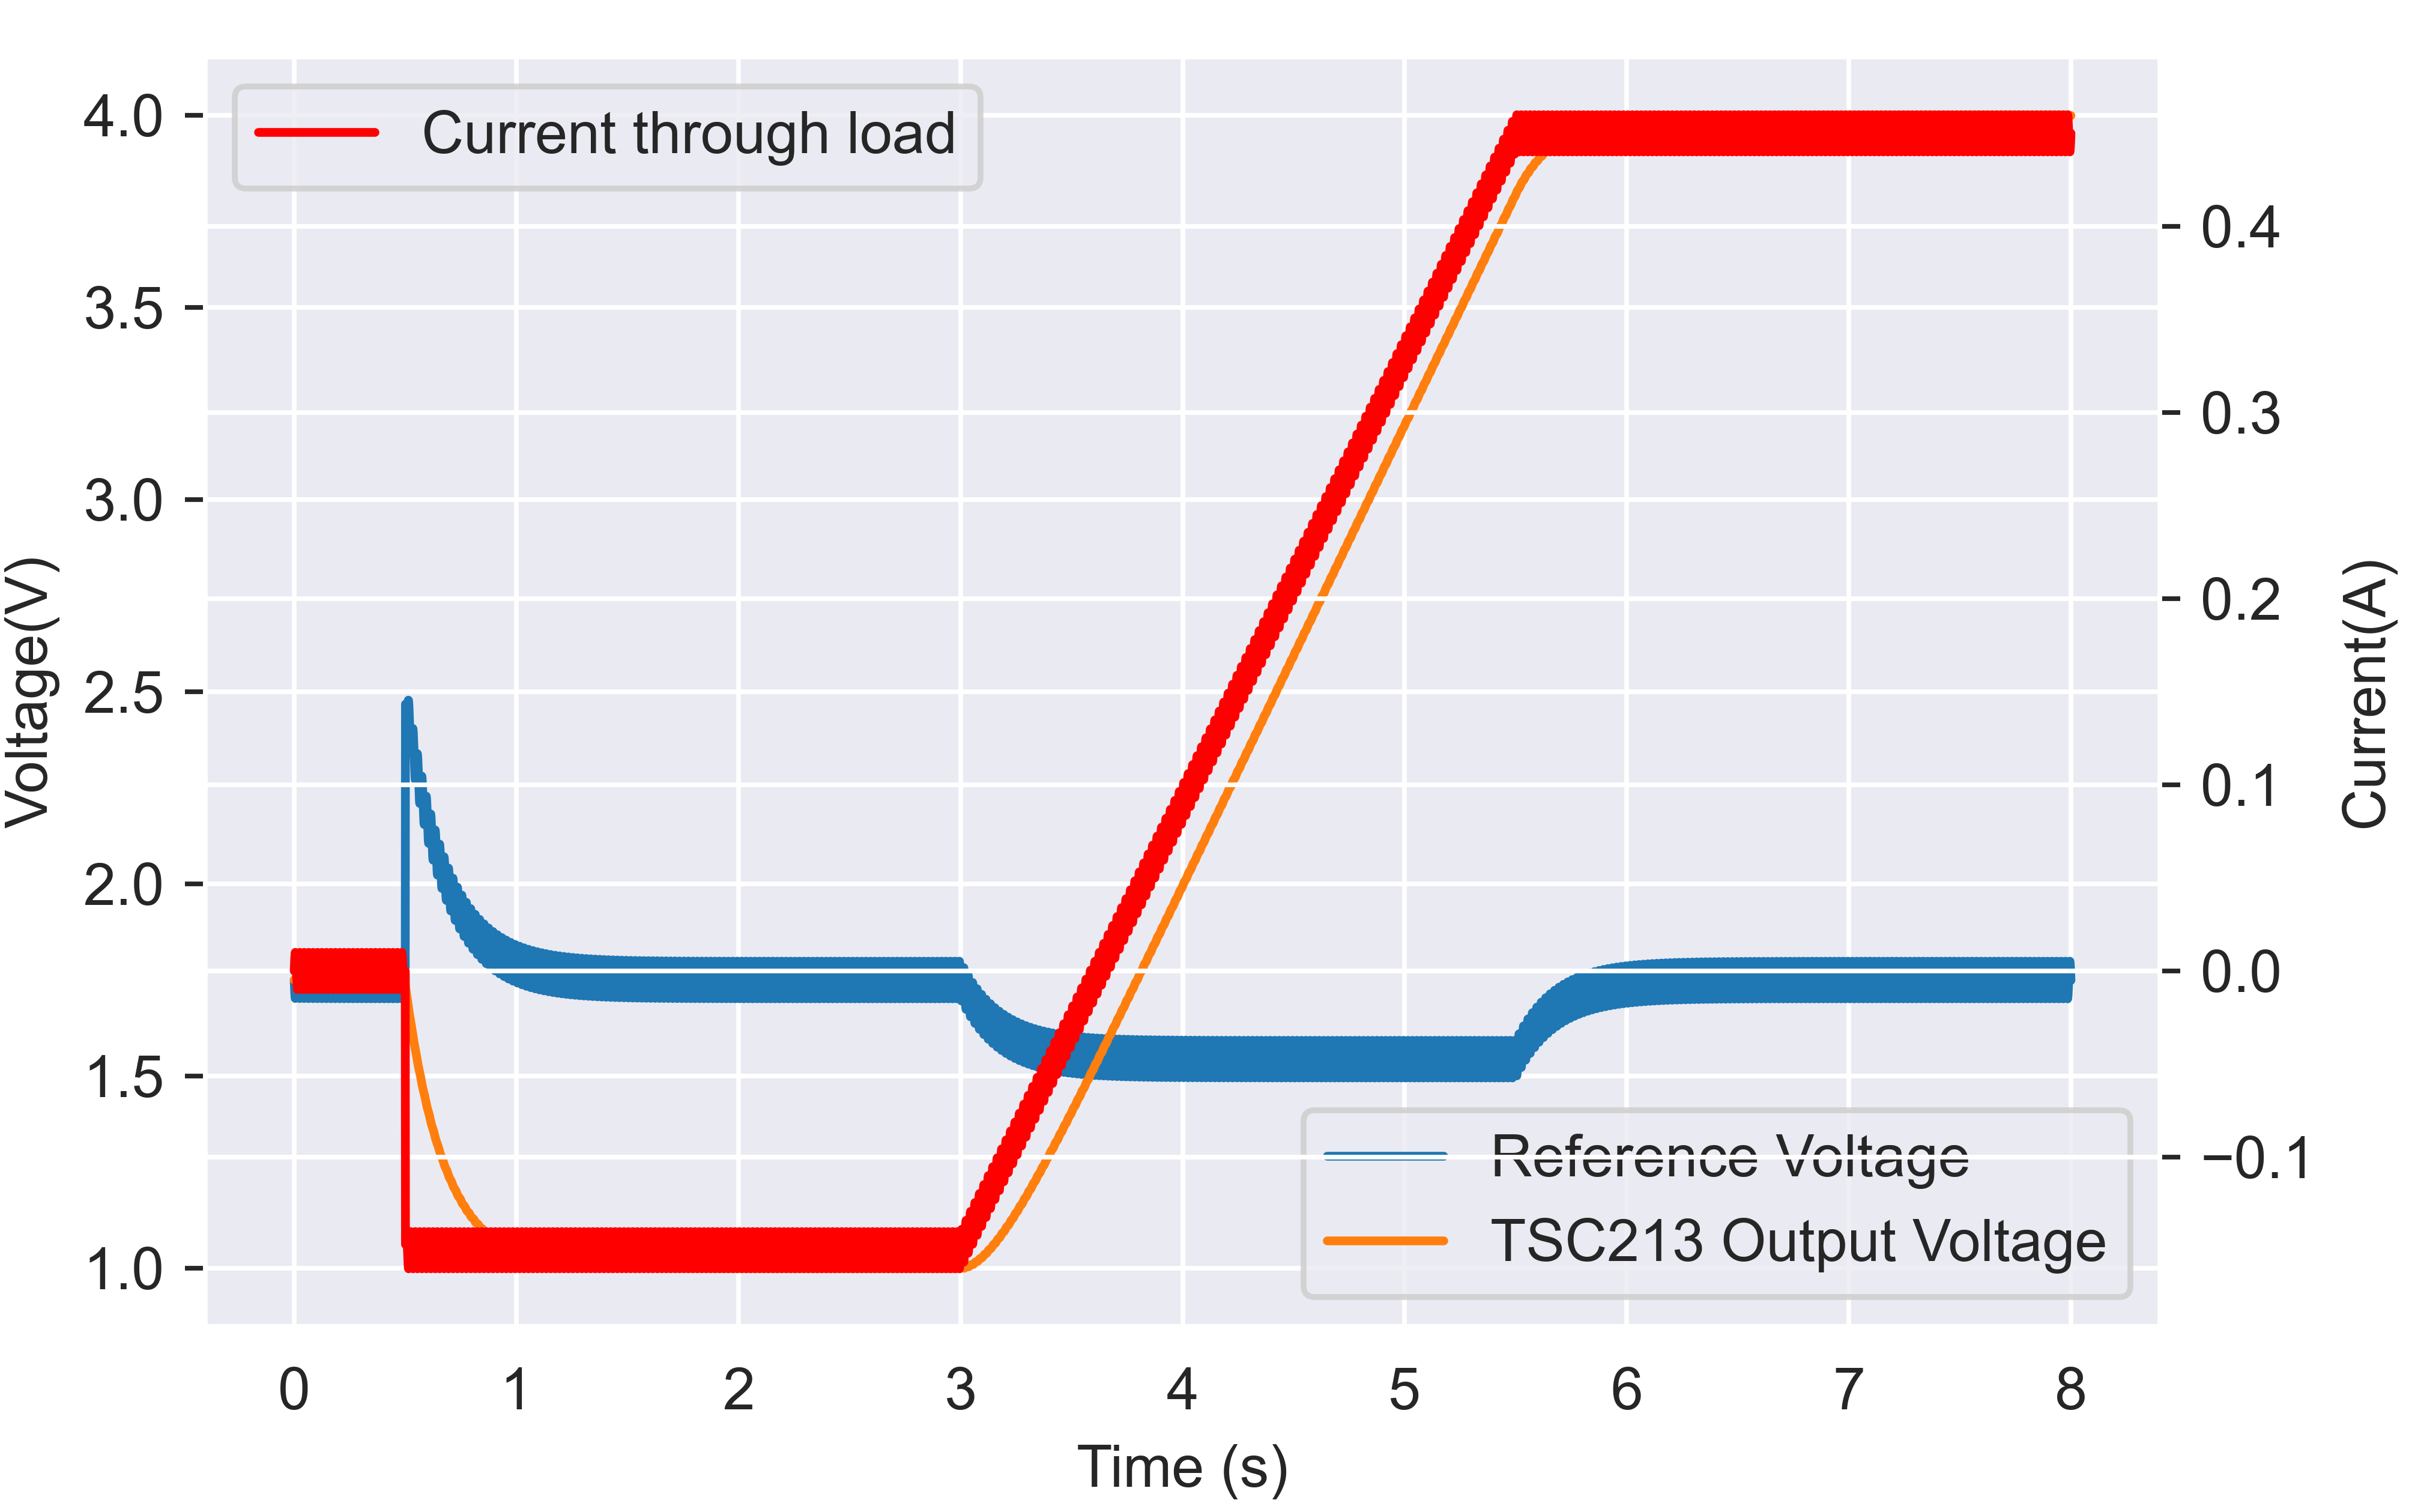
\includegraphics[width=1\linewidth]{./Figures/circuit.png}
		    \caption{} \label{subfig:sim}
     \end{subfigure}
     \begin{subfigure}[]{0.5\textwidth}
             \centering
  		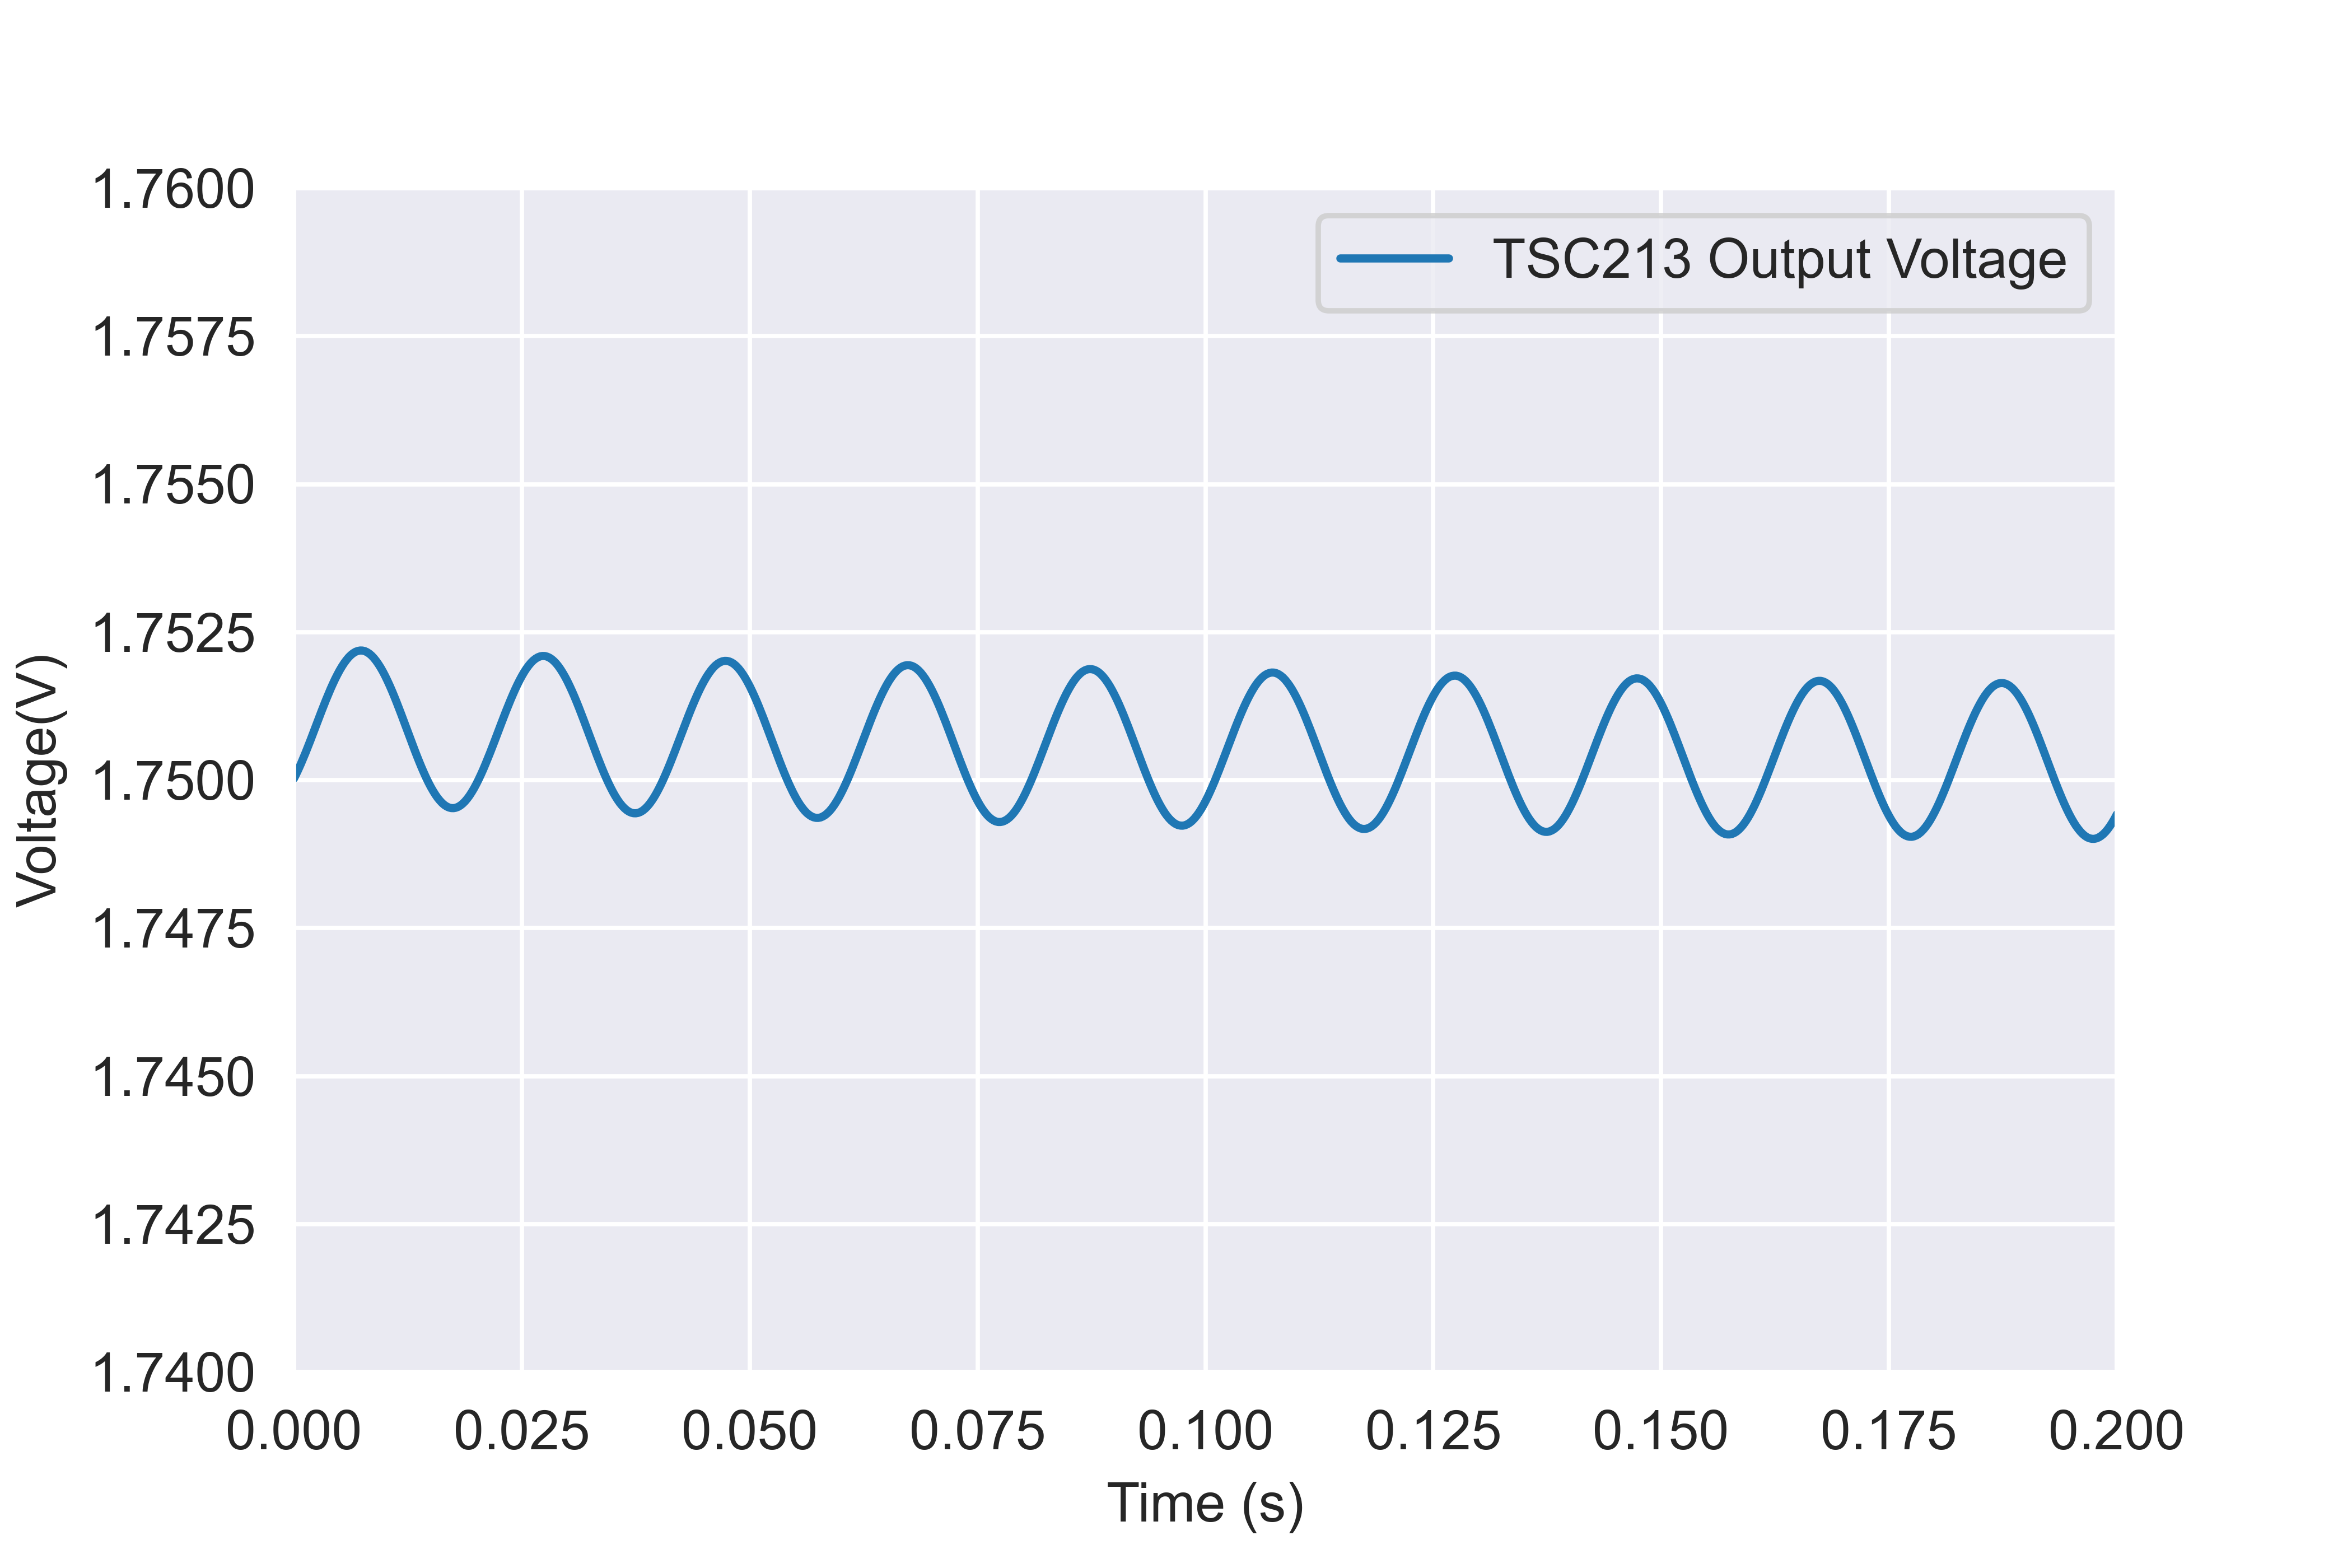
\includegraphics[width=1\linewidth]{./Figures/noise.png}
		   \caption{ } \label{subfig:noise}
     \end{subfigure}
   \caption[{Current Sense LTSpice Results}]{LT Spice results   (a)  Simulation results (b)Noise in output signal }
 
 \end{figure}

From figures \ref{subfig:noise} and \ref{subfig:sim} it can be seen that the necessary noise specifications are achieved and that the correct output range of 3V lies within the 0-5V boundary.
\begin{figure}[!htb]
\centering
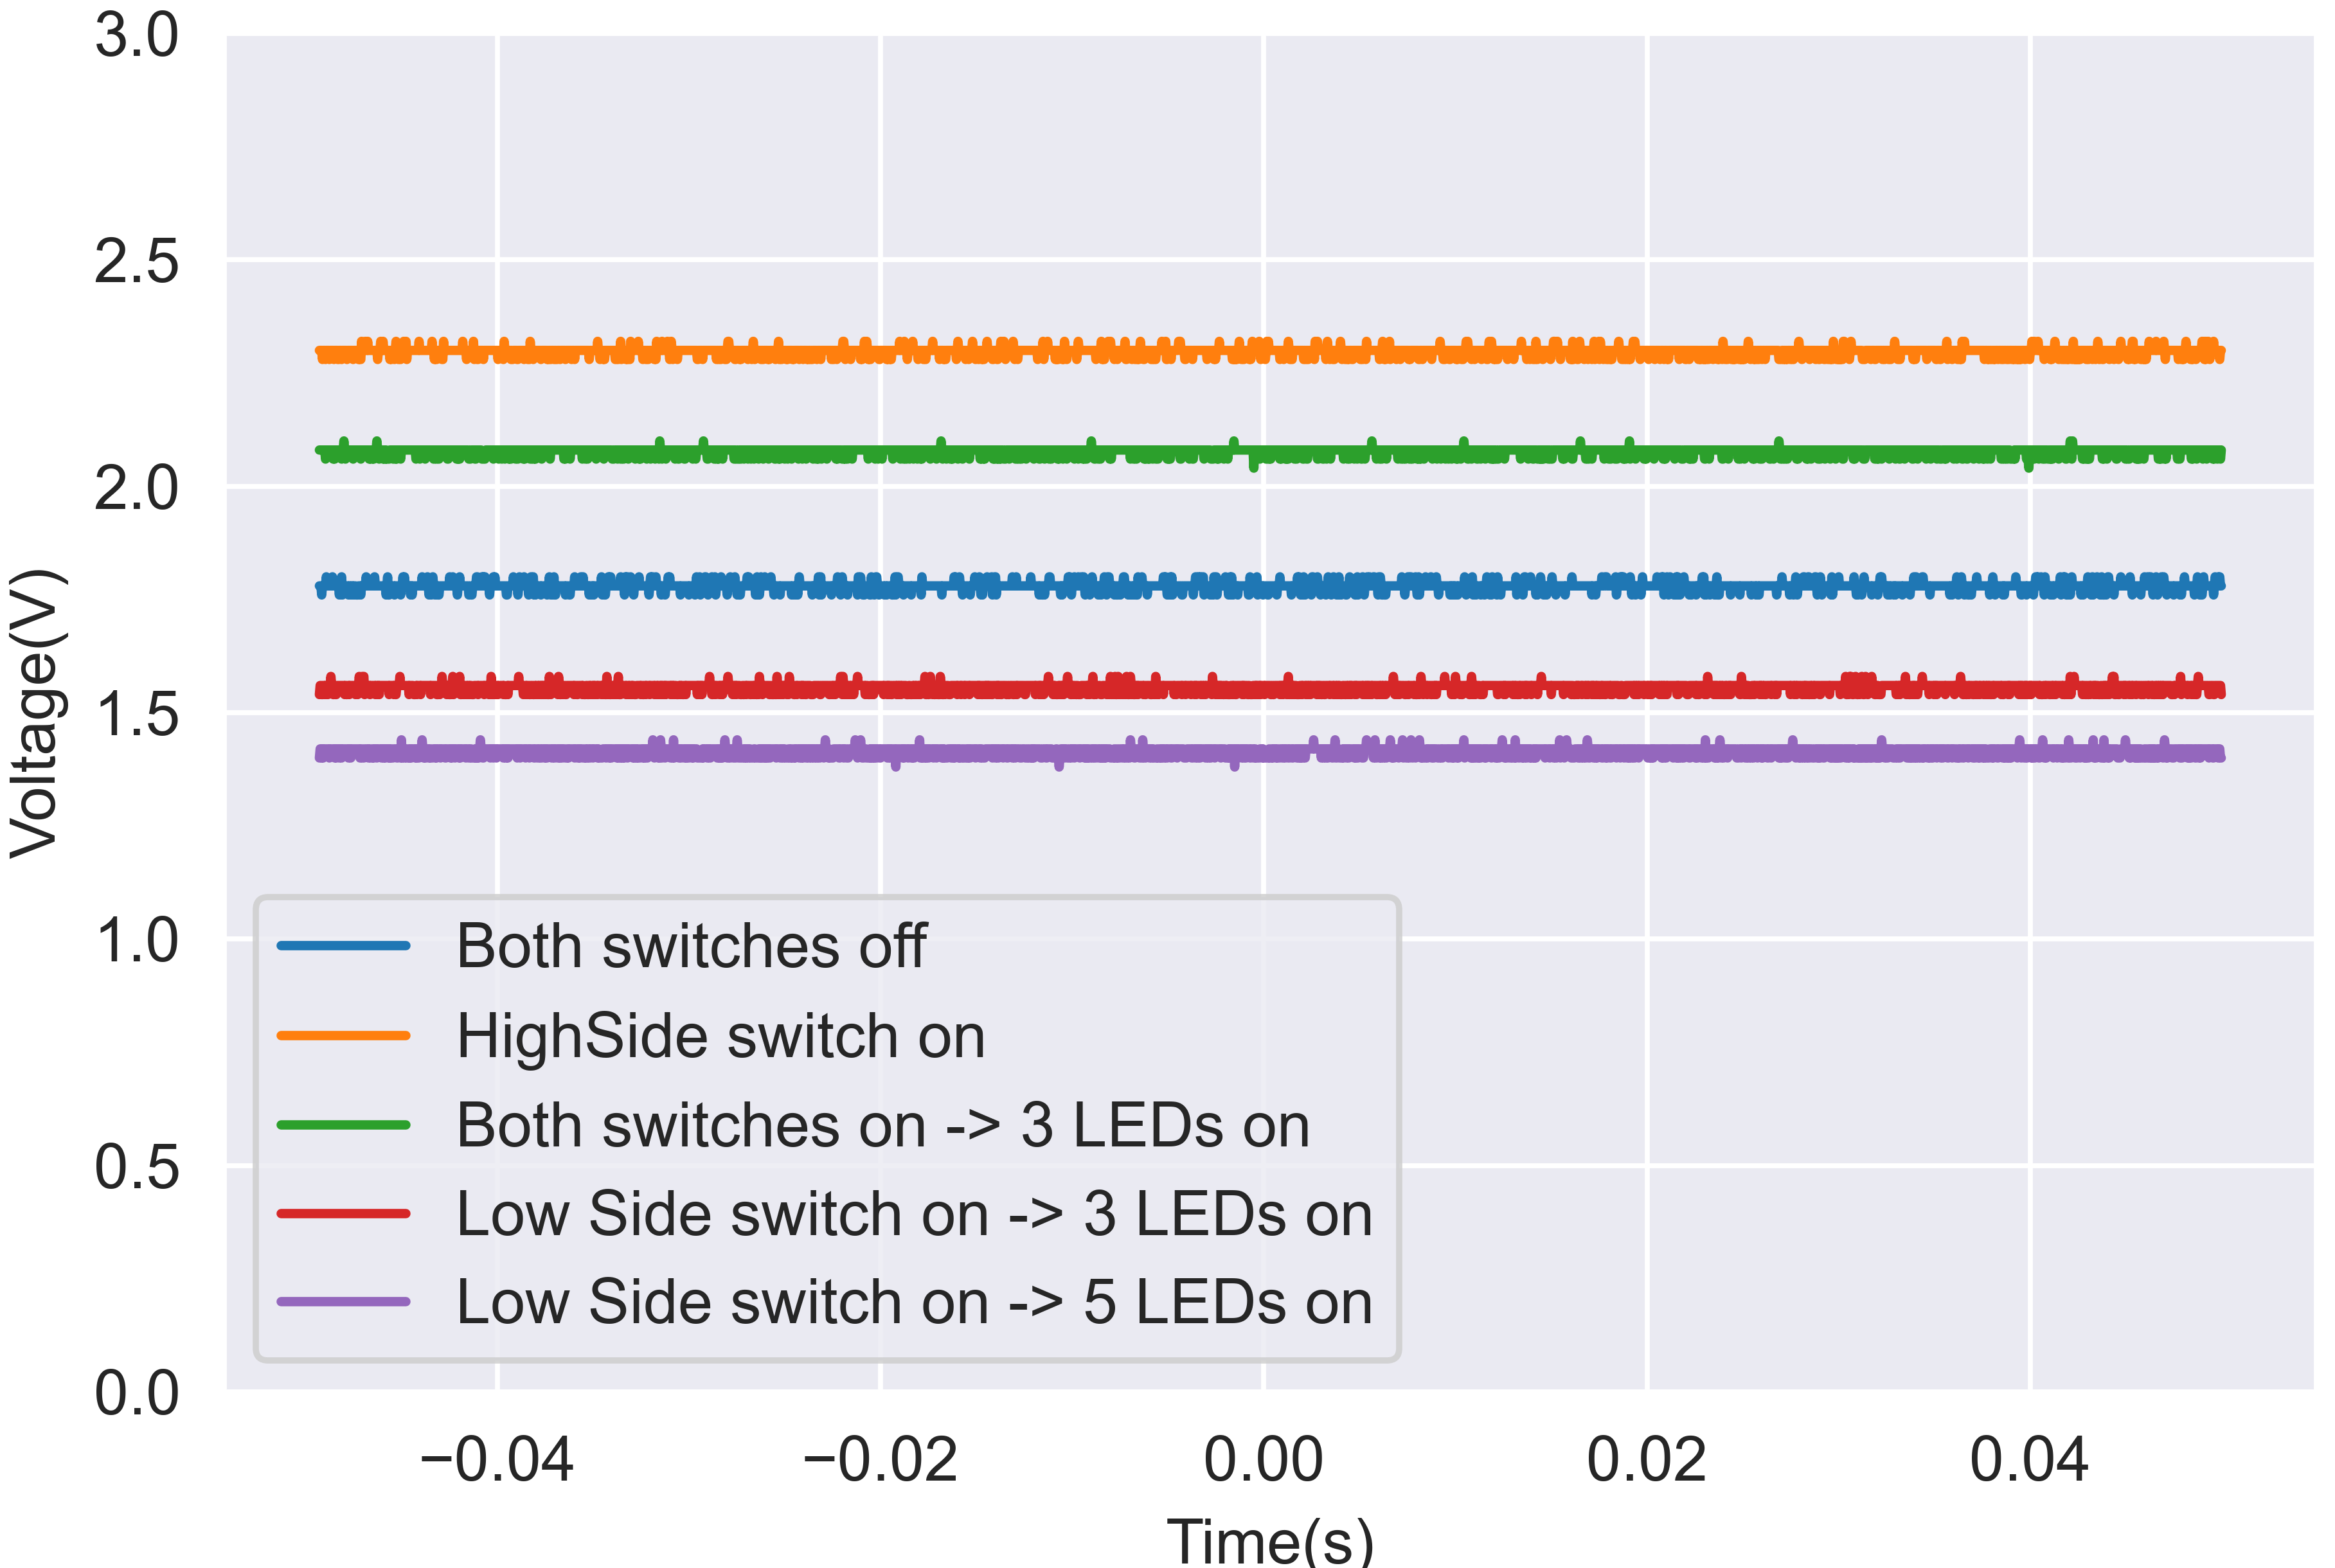
\includegraphics[scale=0.7]{./Figures/meas.png}
\caption{Oscilloscope measurements with various switch states}
\label{fig:meas}
\end{figure}

For the following explanation eq.\ref{eq:refeq} will help explain reasoning. When both switches are off the current flowing through the sense resistor is 0A as can be seen in figure \ref{fig:meas}.For this reason the output is equal to the reference voltage. When the High side switch turns on a positive current flows through the sense resistor, therefore the output increases. As the low side switch switches on, both switches are now on. The output voltage is still higher than the reference voltage because the charging current is greater than the discharging current resulting in a net positive current flow. When the high side switch then turns off the output voltage moves to below the reference voltage because now there is a net negative current through the resistor. As the last 2 LEDs are turned on the output of the TSC213 drops further as the negative (discharging) current increases.



\begin{table}[!htb]
        \centering
        \footnotesize
        \caption{Resistor measurements}
         \begin{tabular}{lrrrr}
          \toprule
             & $Resistor \ Voltage$ & $Calculated \ Current$ \\
             &  [V]  & [mA]\\
          \midrule
         R1      & 3.35 & 15.23 \\
          R2 & 3.34   & 15.18 \\
          R3       &3.36 & 15.27 \\
          R4        &3.35 & 15.23 \\
          R4        &3.37 &15.32 \\
          \bottomrule
        \end{tabular}
     \label{tab:resistor meas}
\end{table}



\begin{table}[!htb]
        \centering
        \footnotesize
        \caption{Measured results compared to actual results}
         \begin{tabular}{lrrrr}
          \toprule
             & TSC213 output voltage&Measured current flow & Indicated current flow& Error \\
             &   [V]&[mA]  &[mA]&[\%]\\
          \midrule
         Both switches off      & 1.75 &0 &0 &0 \\
         Low side switch on(3 LEDs)     & 1.525 & 45.8&45 &1.75 \\
         Low side switch on(5 LEDs)    & 1.383 & 73.4&76.2 &3.85 \\
          
          \bottomrule
        \end{tabular}
     \label{tab:compare}
\end{table}
The LT spice simulations(figure \ref{subfig:sim}) show the output working correctly and the noise( figure \ref{subfig:noise}) is within spec. The measured noise on the output of the TSC213 was found to be 40mV ($V_{PK-PK}$) on the oscilloscope. Larger capacitors were added to try reduce the noise, this was not successful. When the wall plug was powered off and only the battery was supplying the peak to peak voltage dropped to 8mV. This then identified the largest source of noise as the wall plug. Once again a large capacitor was used to try filter out the noise from the 12V, however this also did not decrease the output noise. The current through the LEDs is slightly less than 20mA as can be seen in table \ref{tab:resistor meas} as a result of the resistors chose in section \ref{sec:loadcontrol_design}. Regardless of the noise relatively accurate current measurements were obtained from the TSC213 output as can be seen in table \ref{tab:compare}.

%%%%%%%%%%%%%%%%%%%%%%%%%%%%%%%%%%%%%%%%%%%%%%%%%
\newpage
\section{Low-side switch}
\label{sec:loadcontrol_results}
 \begin{figure}[!htb]
 \footnotesize
 \centering
    \begin{subfigure}[]{0.42\textwidth}
              \centering
  		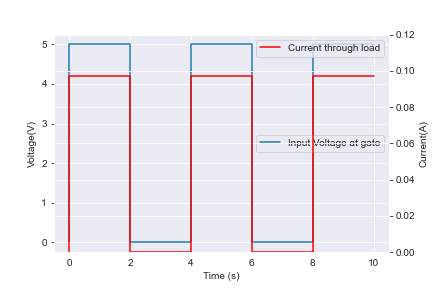
\includegraphics[width=1\linewidth]{./Figures/NMOS.png}
		    \caption{} \label{subfig:nmosfig}
     \end{subfigure}
     \begin{subfigure}[]{0.3\textwidth}
             \centering
  		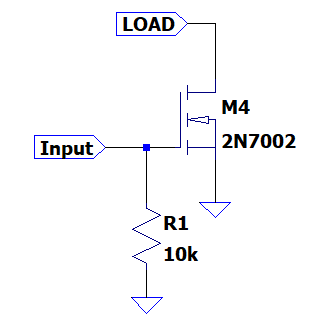
\includegraphics[width=1\linewidth]{./Figures/circNMOS.png}
		   \caption{ } \label{subfig:circnmos}
     \end{subfigure}
   \caption[{NMOS final results}]{NMOS final Results   (a)  LT Spice simulation (b)Lowside circuit used }
    \label{fig:NMOScirc}
 \end{figure}
 The above LTspice simulation in figure \ref{subfig:nmosfig} was setup to have a load that had 100mA flowing through it. It shows that the NMOS was able to switch this amount of current with ease using a 5V control signal. Using this circuit practically the low side switching in figure \ref{fig:meas} was achieved, indicating that it was able to enable and disable discharge through the load.


\begin{figure}[!htb]
\centering
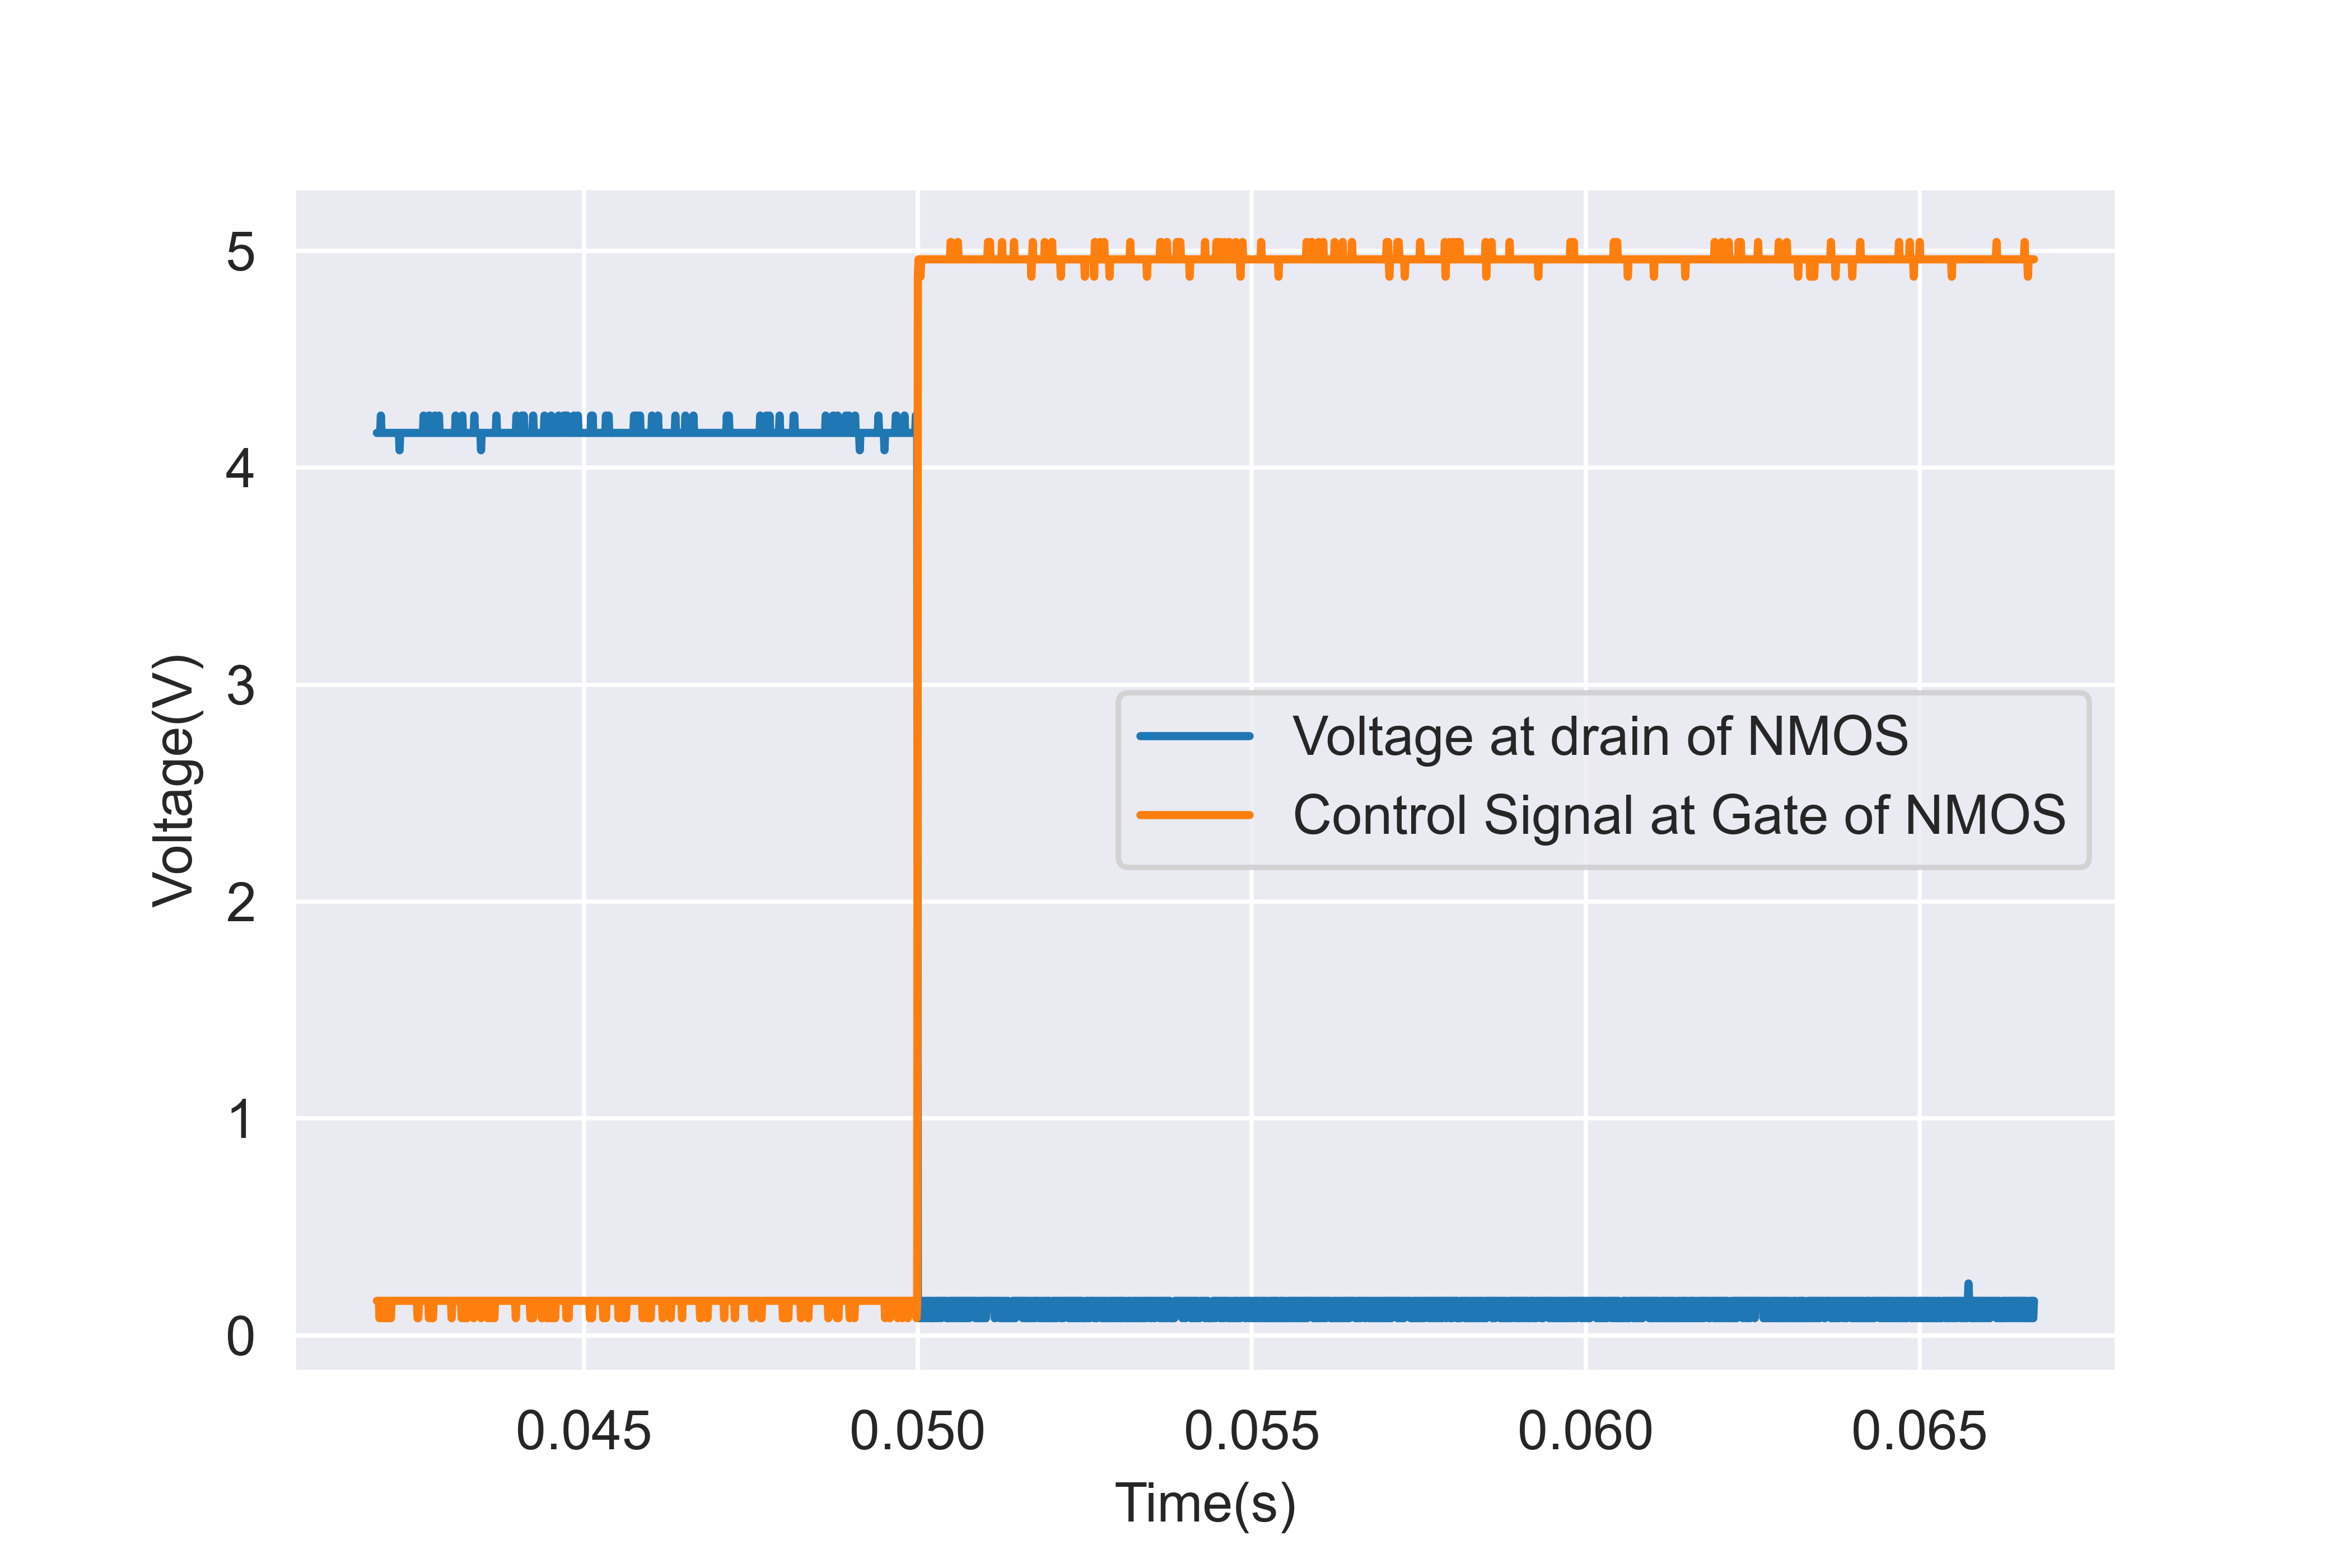
\includegraphics[scale=0.6]{./Figures/NMOSmeas}
\caption{Oscilloscope Measurements of NMOS while switching}
\label{fig:measNMOS}
\end{figure}

From figure \ref{fig:measNMOS} it can be seen that the switching time of the NMOS is virtually instantaneous and also simply that the NMOS switching capability is working correctly. The NMOS source is connected to ground, therefore when the control signal goes high the NMOS "connects" its drain to its source which is ground.

%%%%%%%%%%%%%%%%%%%%%
\newpage
\section{Supply Voltage measurement}


\begin{figure}[!htb]
	\footnotesize
	\centering
	\begin{subfigure}[]{0.48\textwidth}
		\centering
		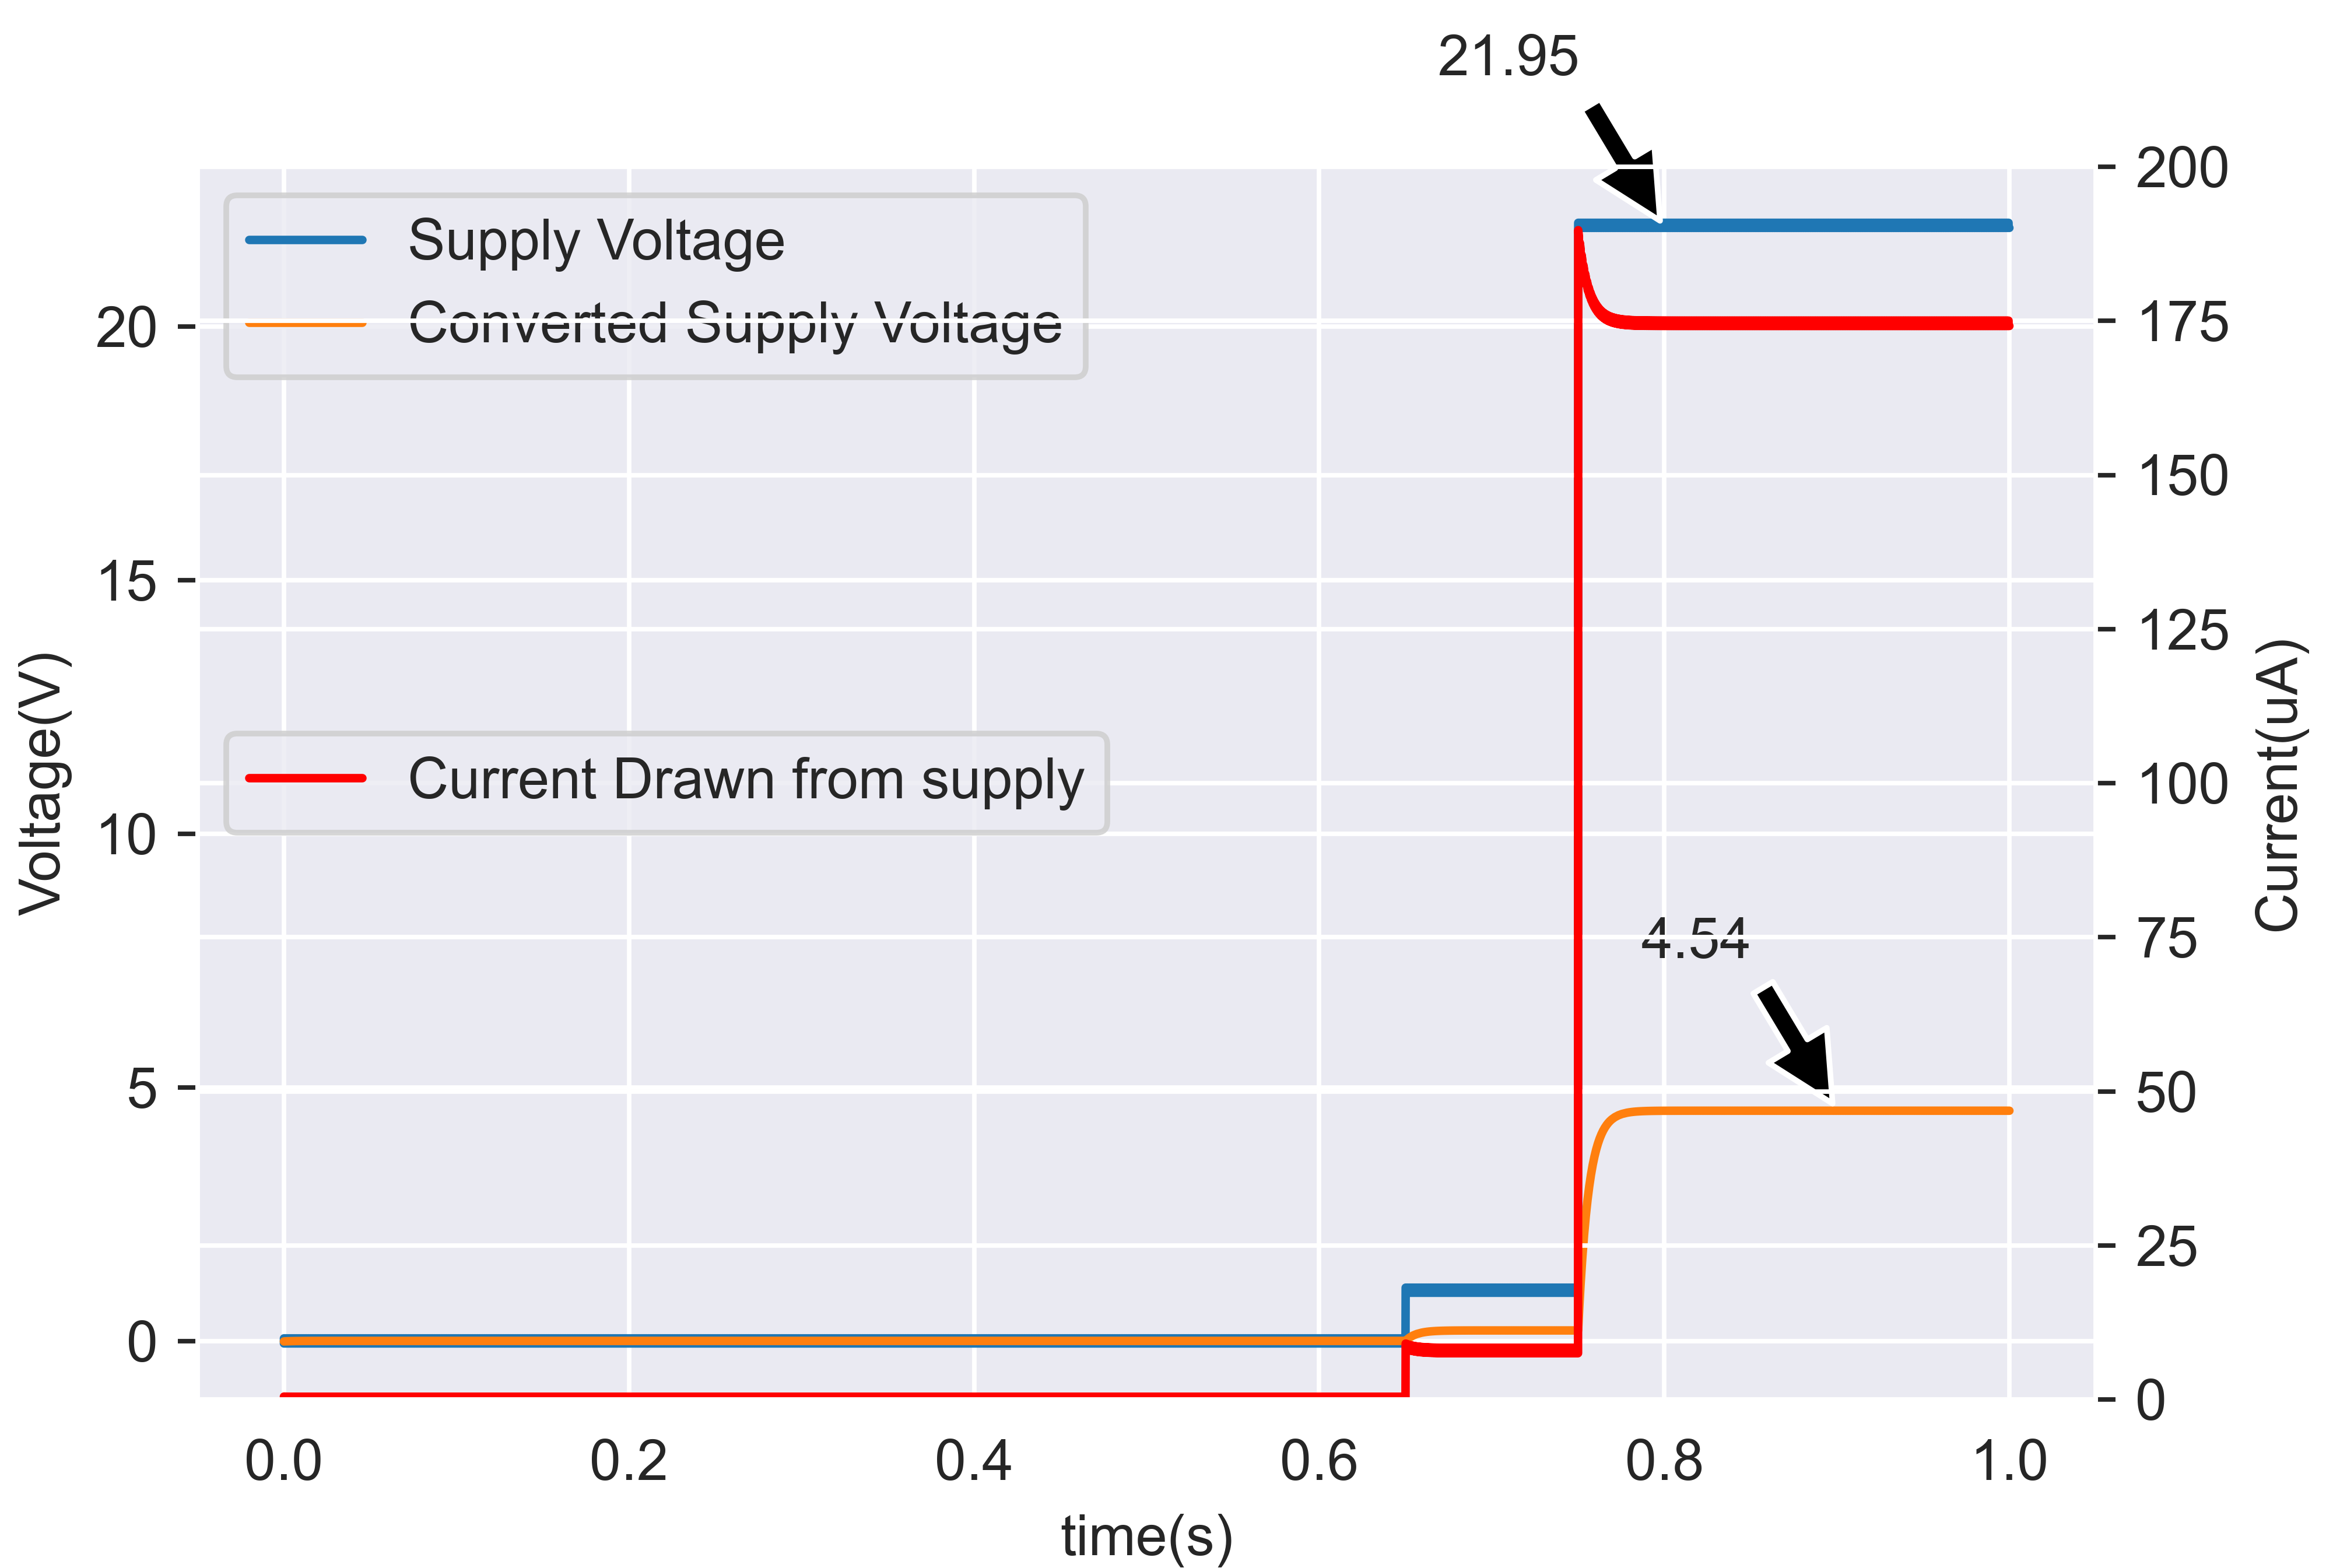
\includegraphics[width=1\linewidth]{./Figures/A6/A6supcurrent.png}
		\caption{} \label{subfig:A6gensup}
	\end{subfigure}
	\begin{subfigure}[]{0.48\textwidth}
		\centering
		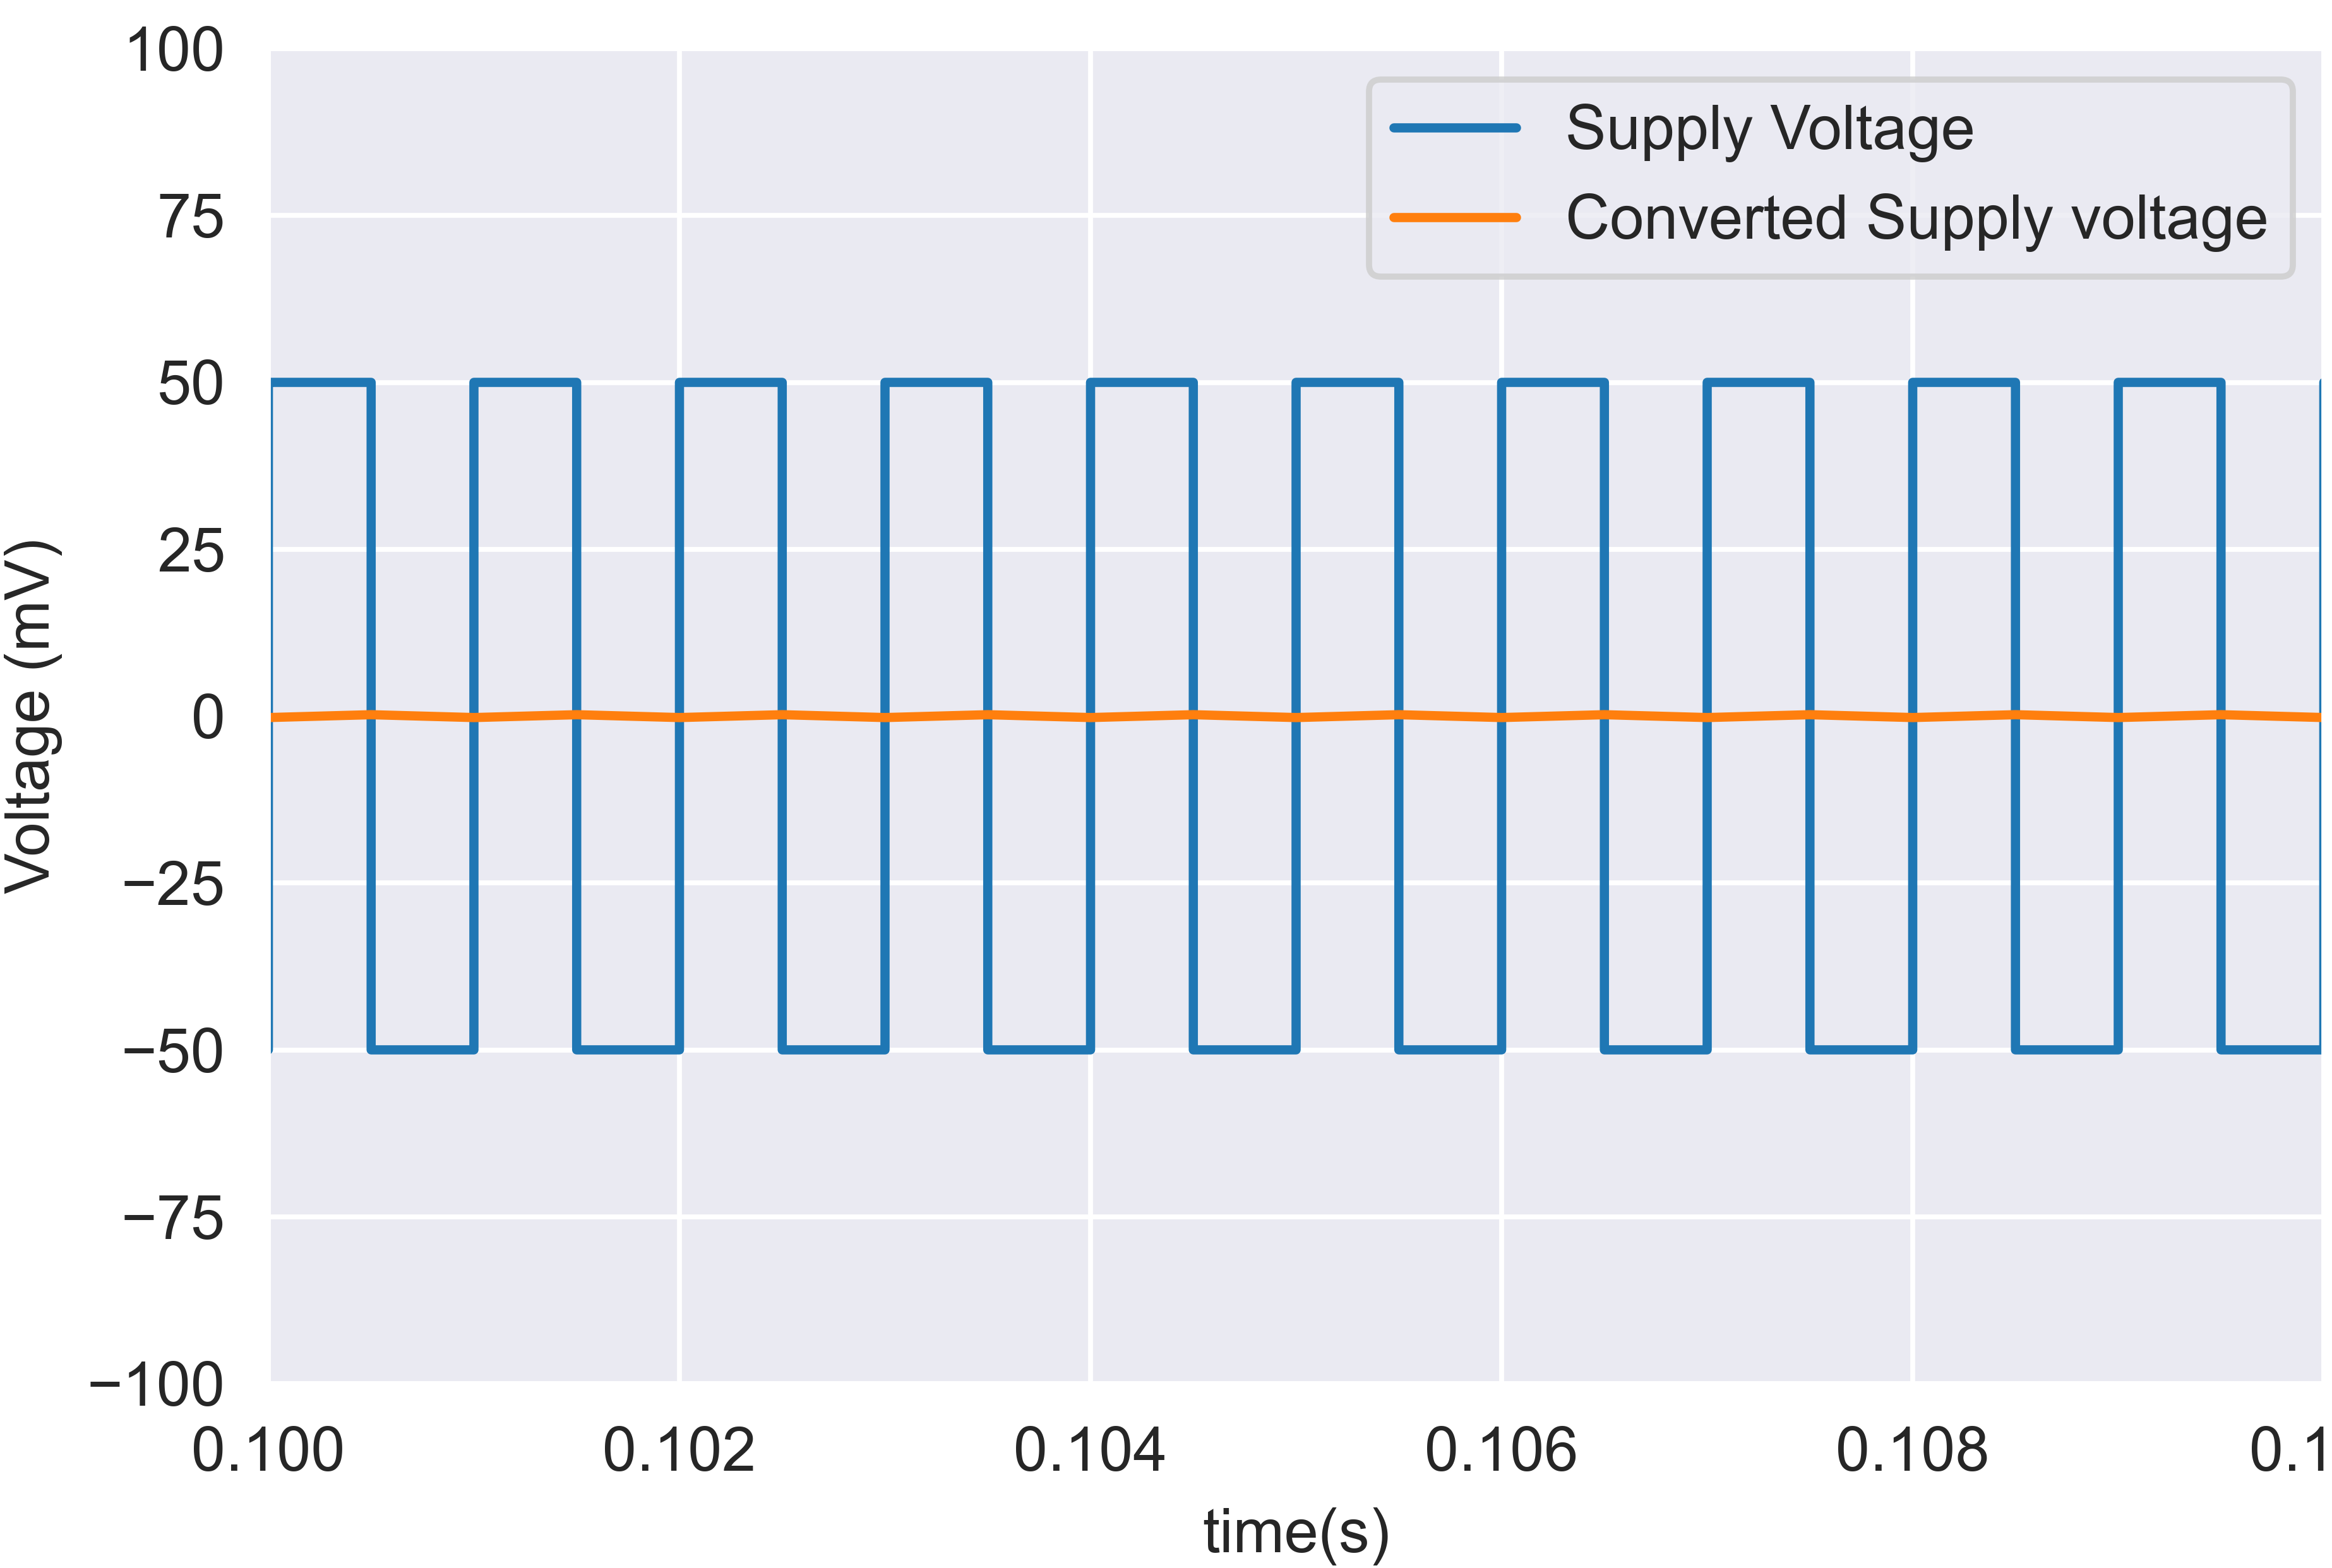
\includegraphics[width=1\linewidth]{./Figures/A6/A6supnoise.png}
		\caption{ } \label{subfig:A6noiselt}
	\end{subfigure}
	\caption[{LTSPICE supply measurement simulation results}]{LTSPICE supply measurement simulation results   (a)  Supply before and after signal conditioning with current drawn from supply (b)Noise on supply input compared to converted supply voltage }
	\label{fig:A6bat}
\end{figure}

From figure \ref{subfig:A6gensup} the converted supply signal is the voltage measured by the ADC. As the supply voltage increases the converted supply signal varies between zero and 4.54V. It does not vary between 0 and exactly 5V because of the additional precaution of 24V as the maximum input voltage where the max input voltage here is 22V. The noise that can be seen in figure  \ref{subfig:A6noiselt} is significantly reduced in the converted signal. The speed of the signal is not severely slowed as can be seen in figure  \ref{subfig:A6gensup} where the converted supply voltage nearly changes 5V in less than 100ms. 




\begin{figure}[!htb]
	\footnotesize
	\centering
	\begin{subfigure}[]{0.4\textwidth}
		\centering
		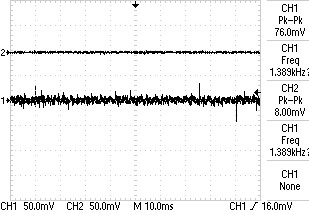
\includegraphics[width=1\linewidth]{./Figures/A6/noisesup.jpg}
		\caption{} \label{subfig:noiseSup}
	\end{subfigure}
	\begin{subfigure}[]{0.4\textwidth}
		\centering
		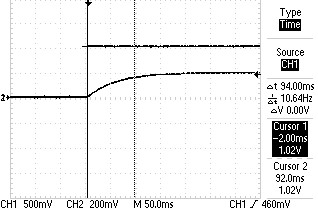
\includegraphics[width=1\linewidth]{./Figures/A6/risesup.jpg}
		\caption{ } \label{subfig:resSup}
	\end{subfigure}
	\caption[{Oscilloscope Measurements of response time and noise of Supply measuring}]{Oscilloscope Measurements of response time and noise of Supply measuring  (a) Input vs Output battery signal noise (b) Response time of converted battery signal }
	\label{fig:A6suposc}
\end{figure}
 From figure \ref{subfig:A6gensup} it can be seen that the rise time for a step input of one volt is only just less than 100ms, and therefore meets the requirements. The noise in figure \ref{subfig:A6noiselt} can be seen to have significantly decreased from 76mV to 8mV giving a significantly cleaner output signal.

%%%%%%%%%%%%%%%%%%%%%%%%%%%%
\newpage
\section{Battery Voltage measurement}



\begin{figure}[!htb]
	\footnotesize
	\centering
	\begin{subfigure}[]{0.386\textwidth}
		\centering
		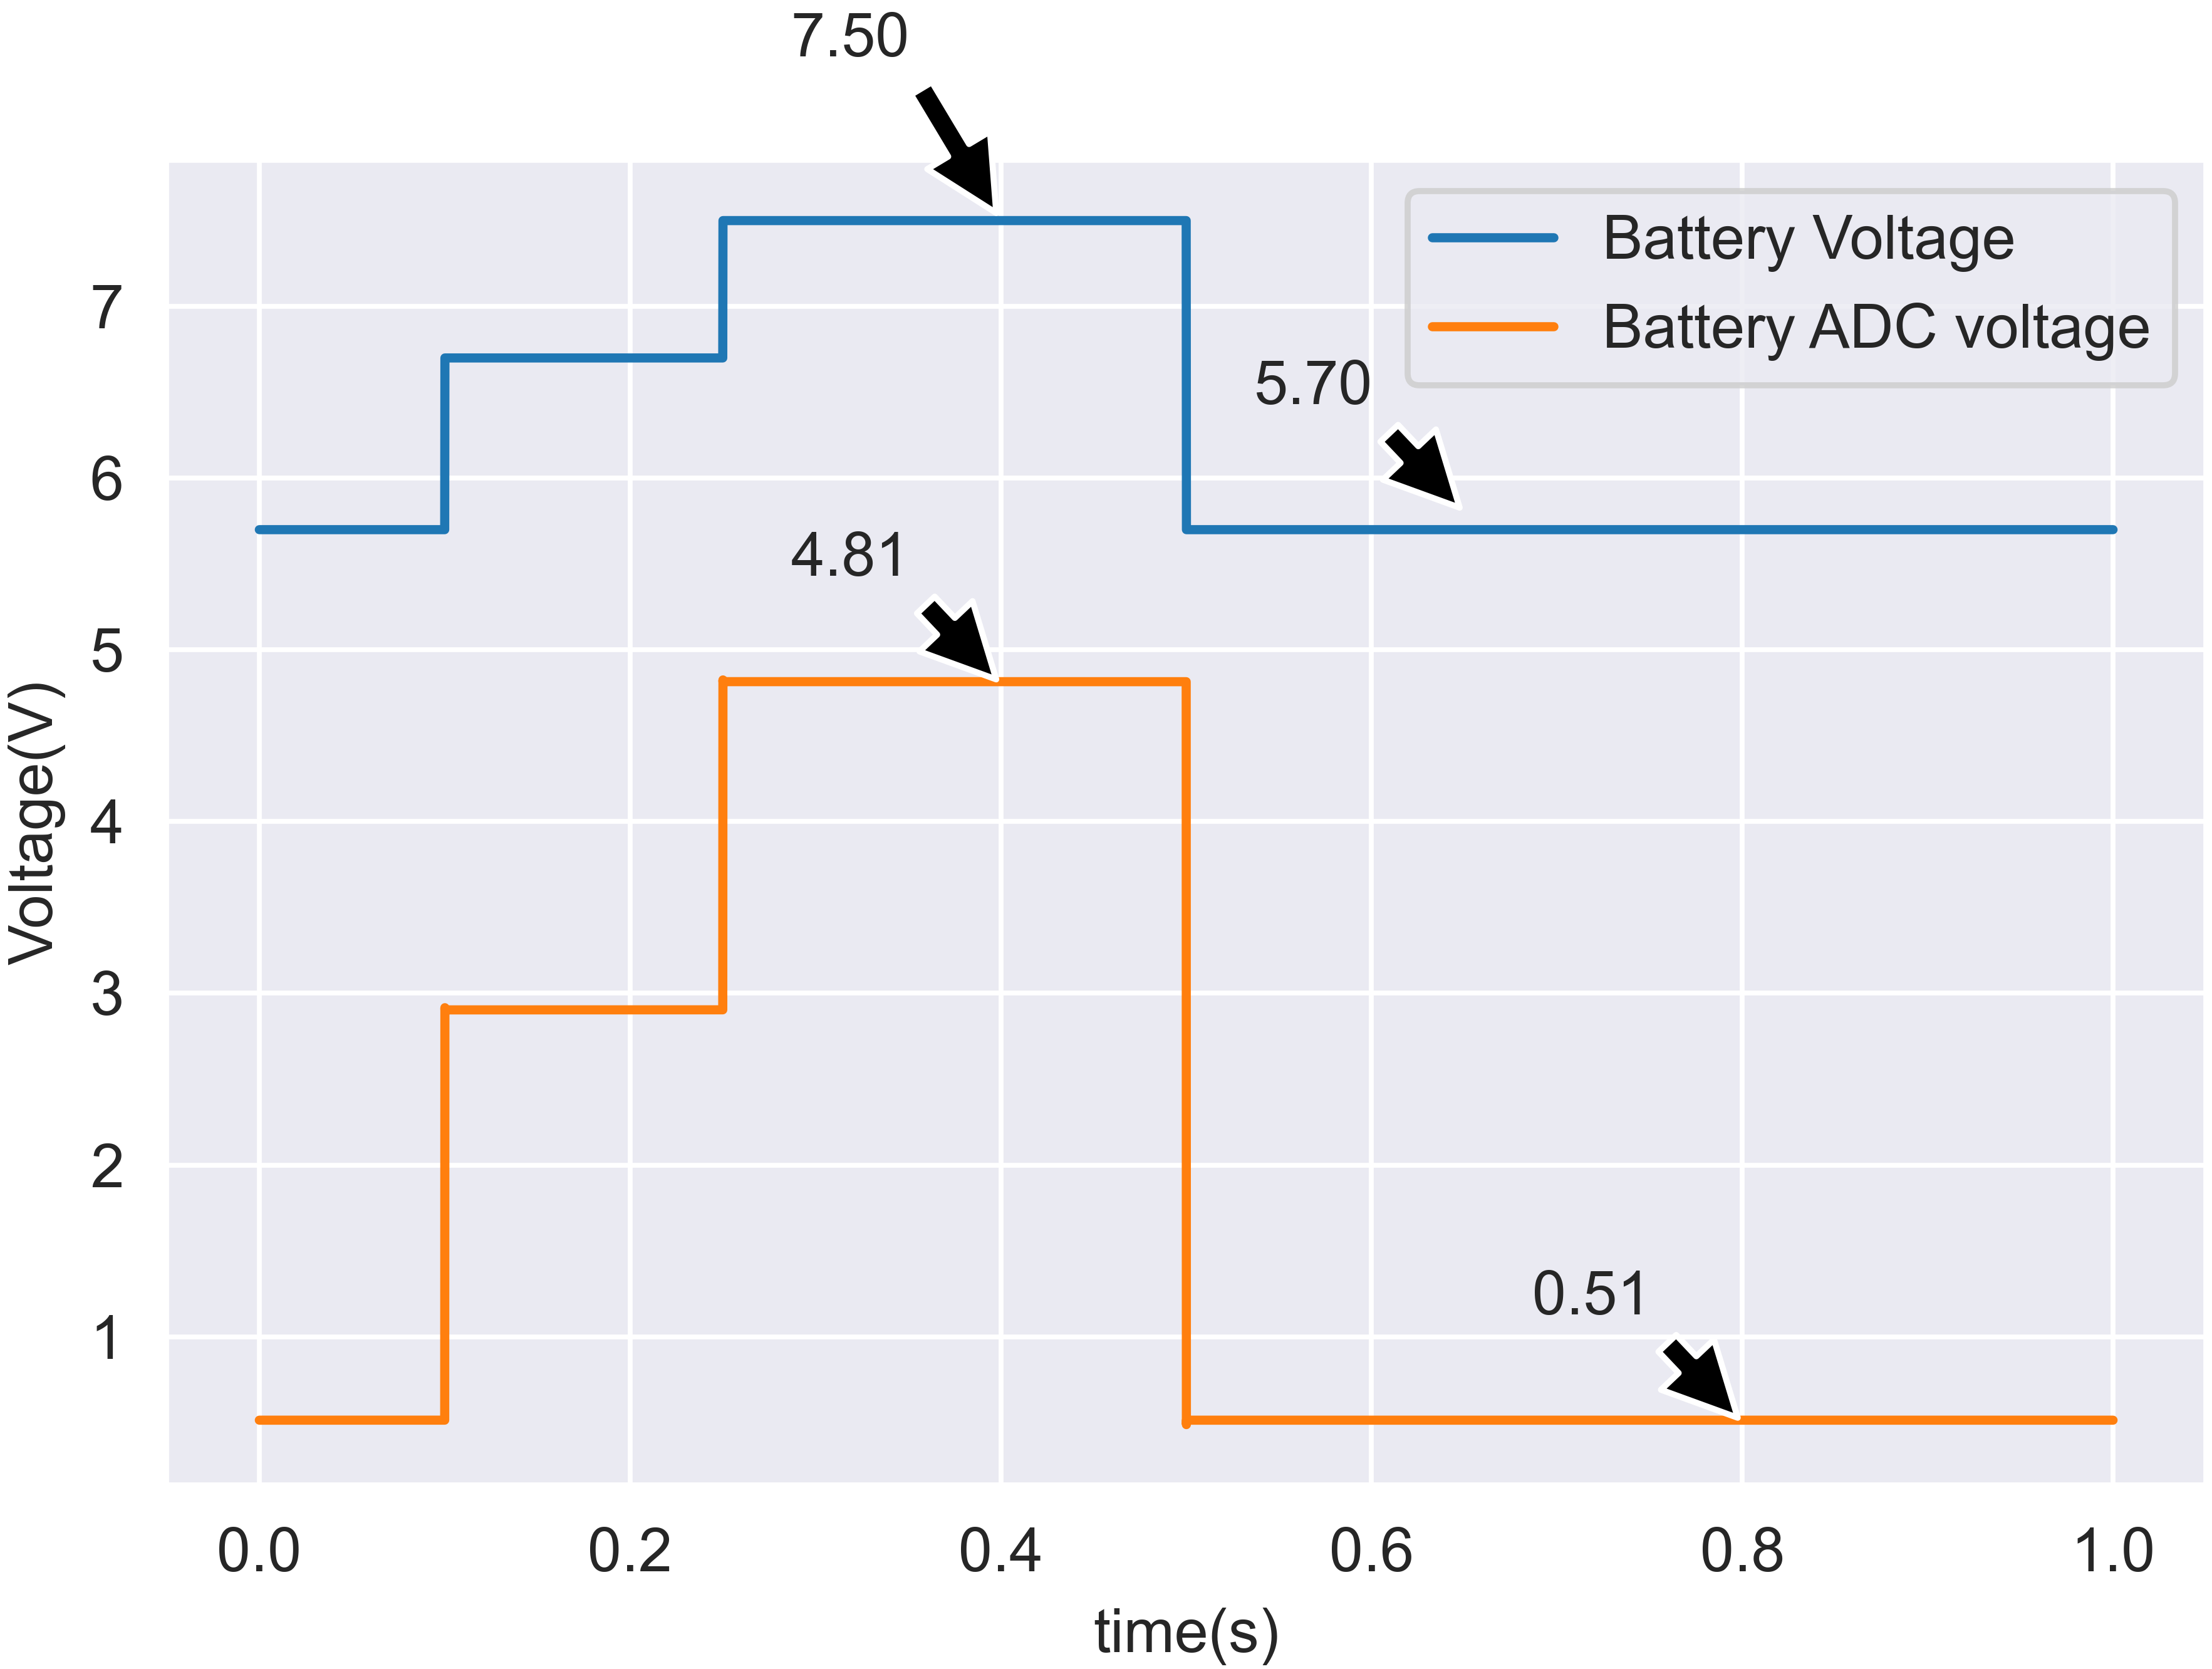
\includegraphics[width=1\linewidth]{./Figures/A6/A6batvolt.png}
		\caption{} \label{subfig:voltbatA6}
	\end{subfigure}
	\begin{subfigure}[]{0.46\textwidth}
		\centering
		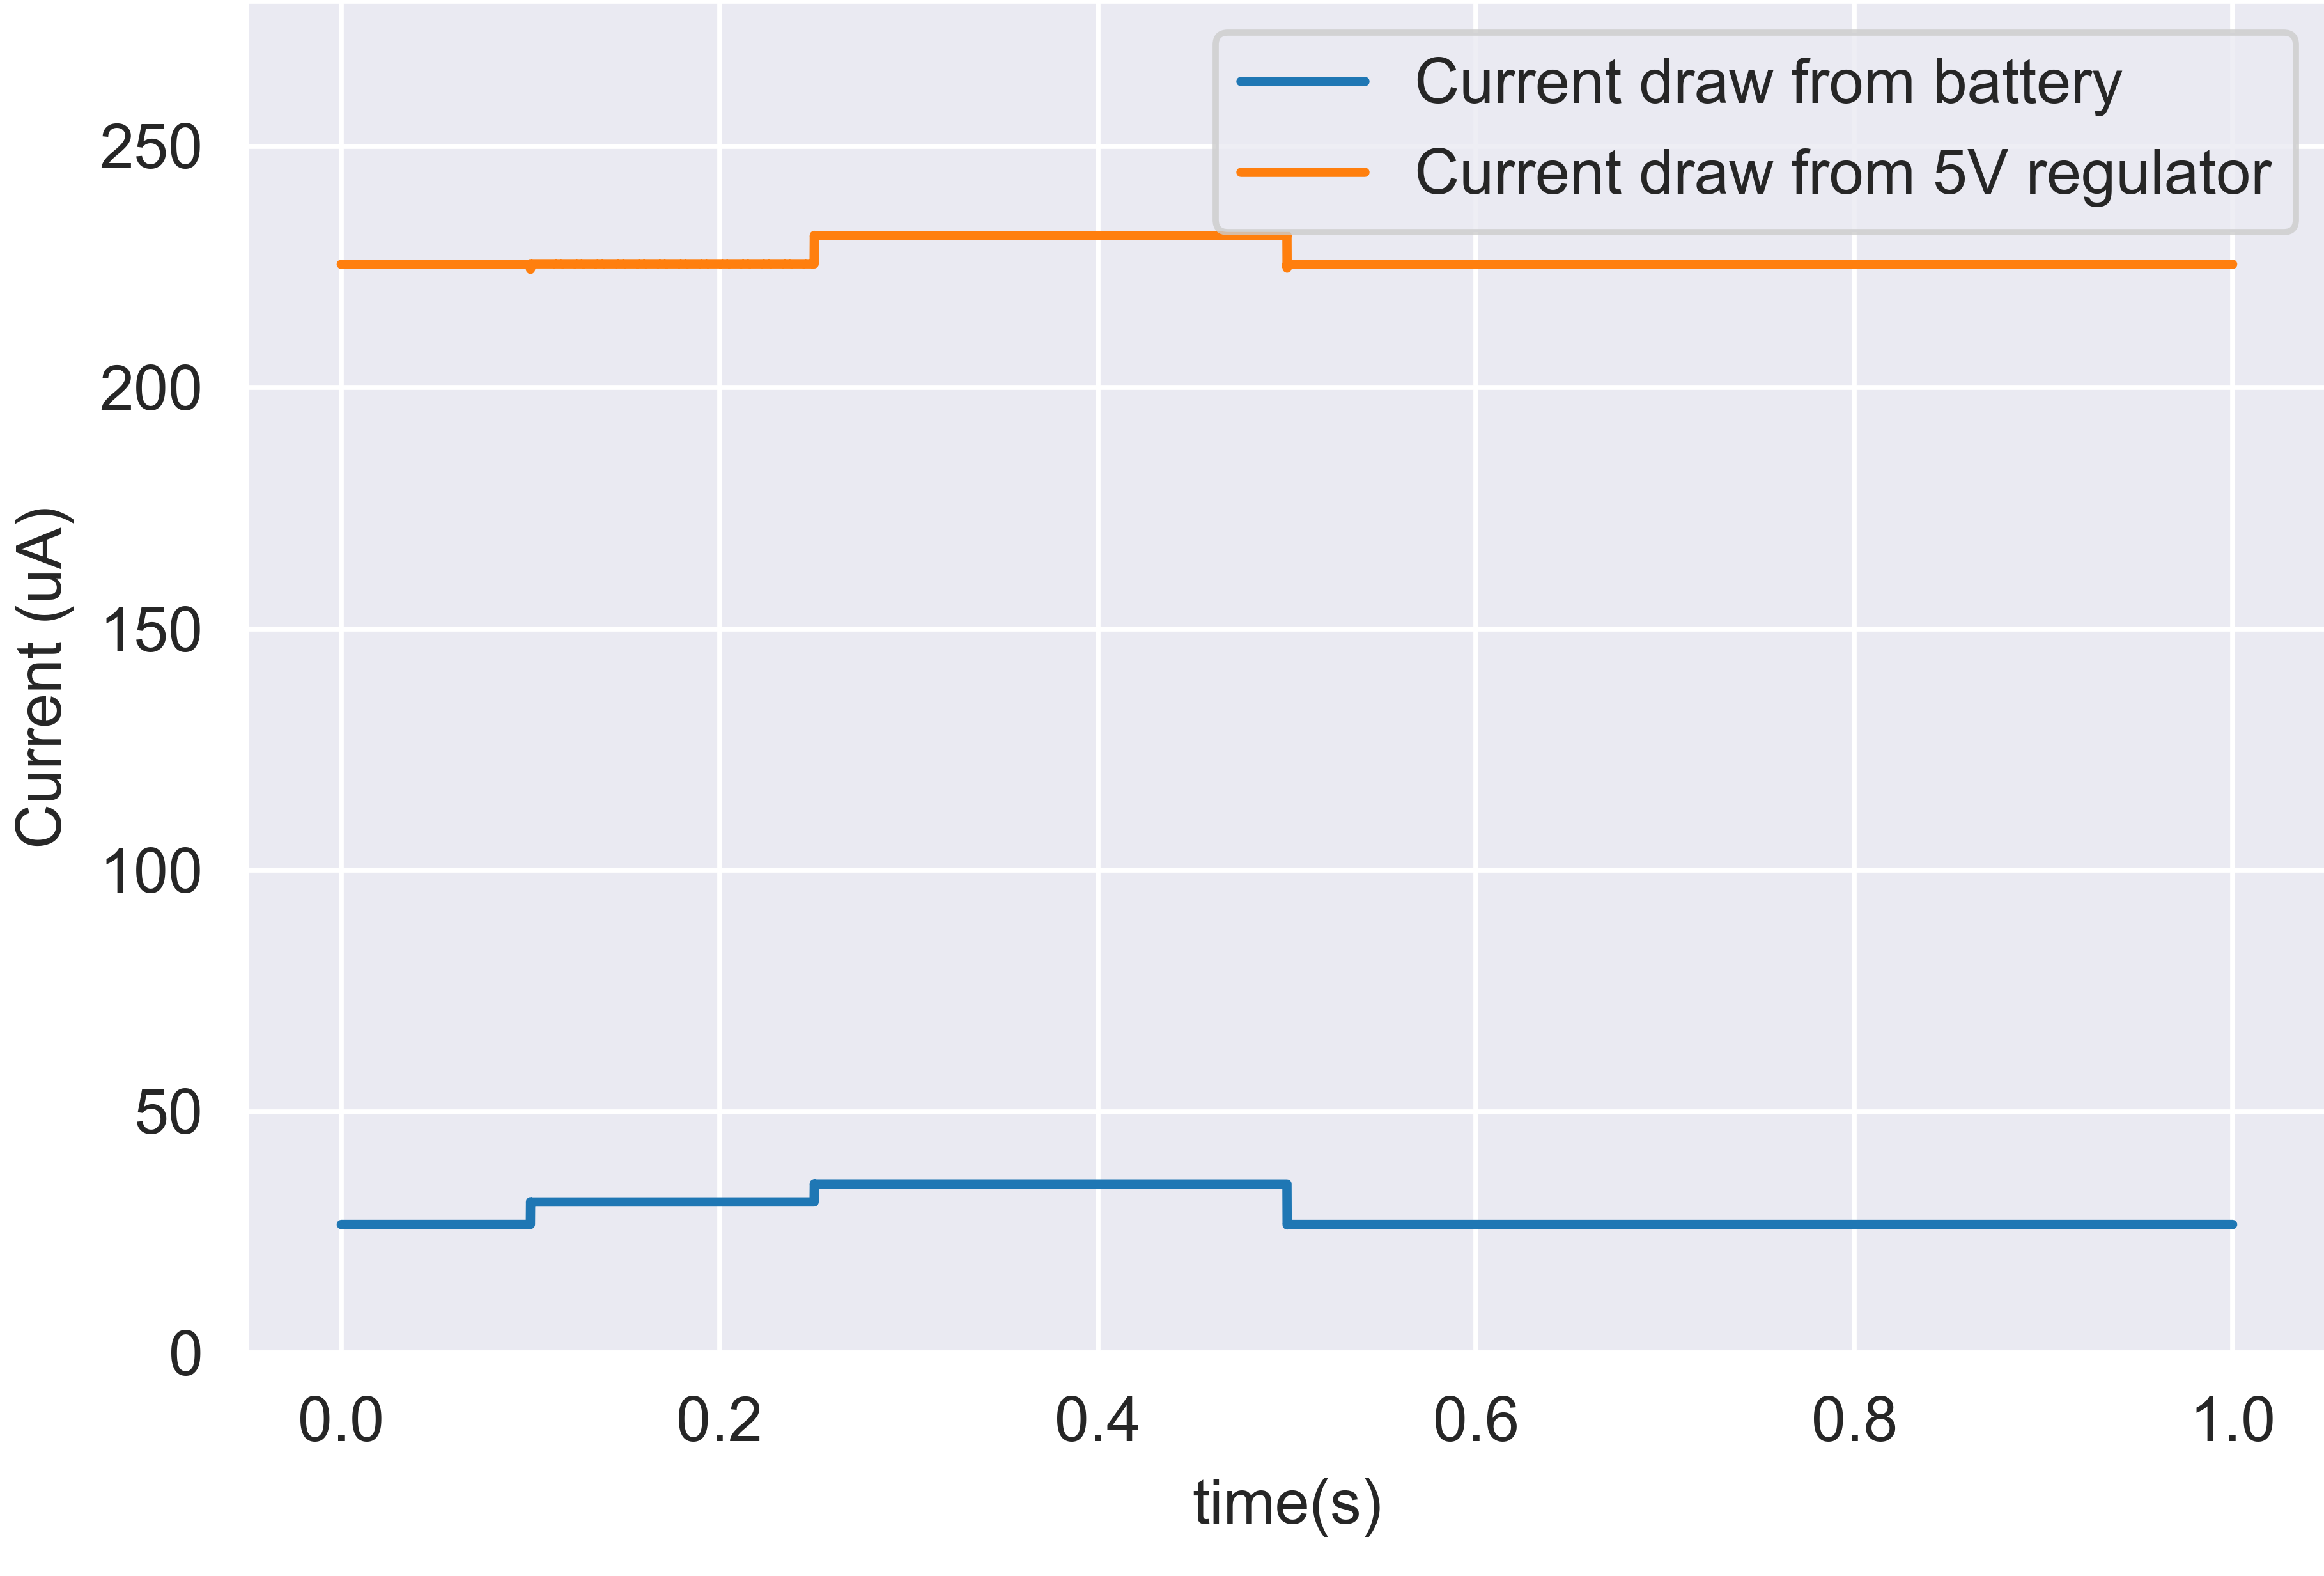
\includegraphics[width=1\linewidth]{./Figures/A6/A6batcurrent.png}
		\caption{ } \label{subfig:currbatA6}
	\end{subfigure}
	\caption[{LTSPICE battery measurement simulation results}]{LTSPICE battery measurement simulation results   (a)  Battery before and after signal conditioning (b)Battery Current and 5V regulator current }
	\label{fig:A6bat}
\end{figure}

From the results seen in figure \ref{subfig:voltbatA6} the ADC battery voltage increases as the battery voltage increases. The ADC battery voltage should vary between 0.5V and 4.8V. The simulation is only 0.01V from the expected values, this is likely a result of resistor values that are chosen. The current drawn from the battery directly as well as indirectly through the 5V regulator sum to less than $300\mu A$ indicating minimal current usage.




\begin{figure}[!htb]
	\centering
	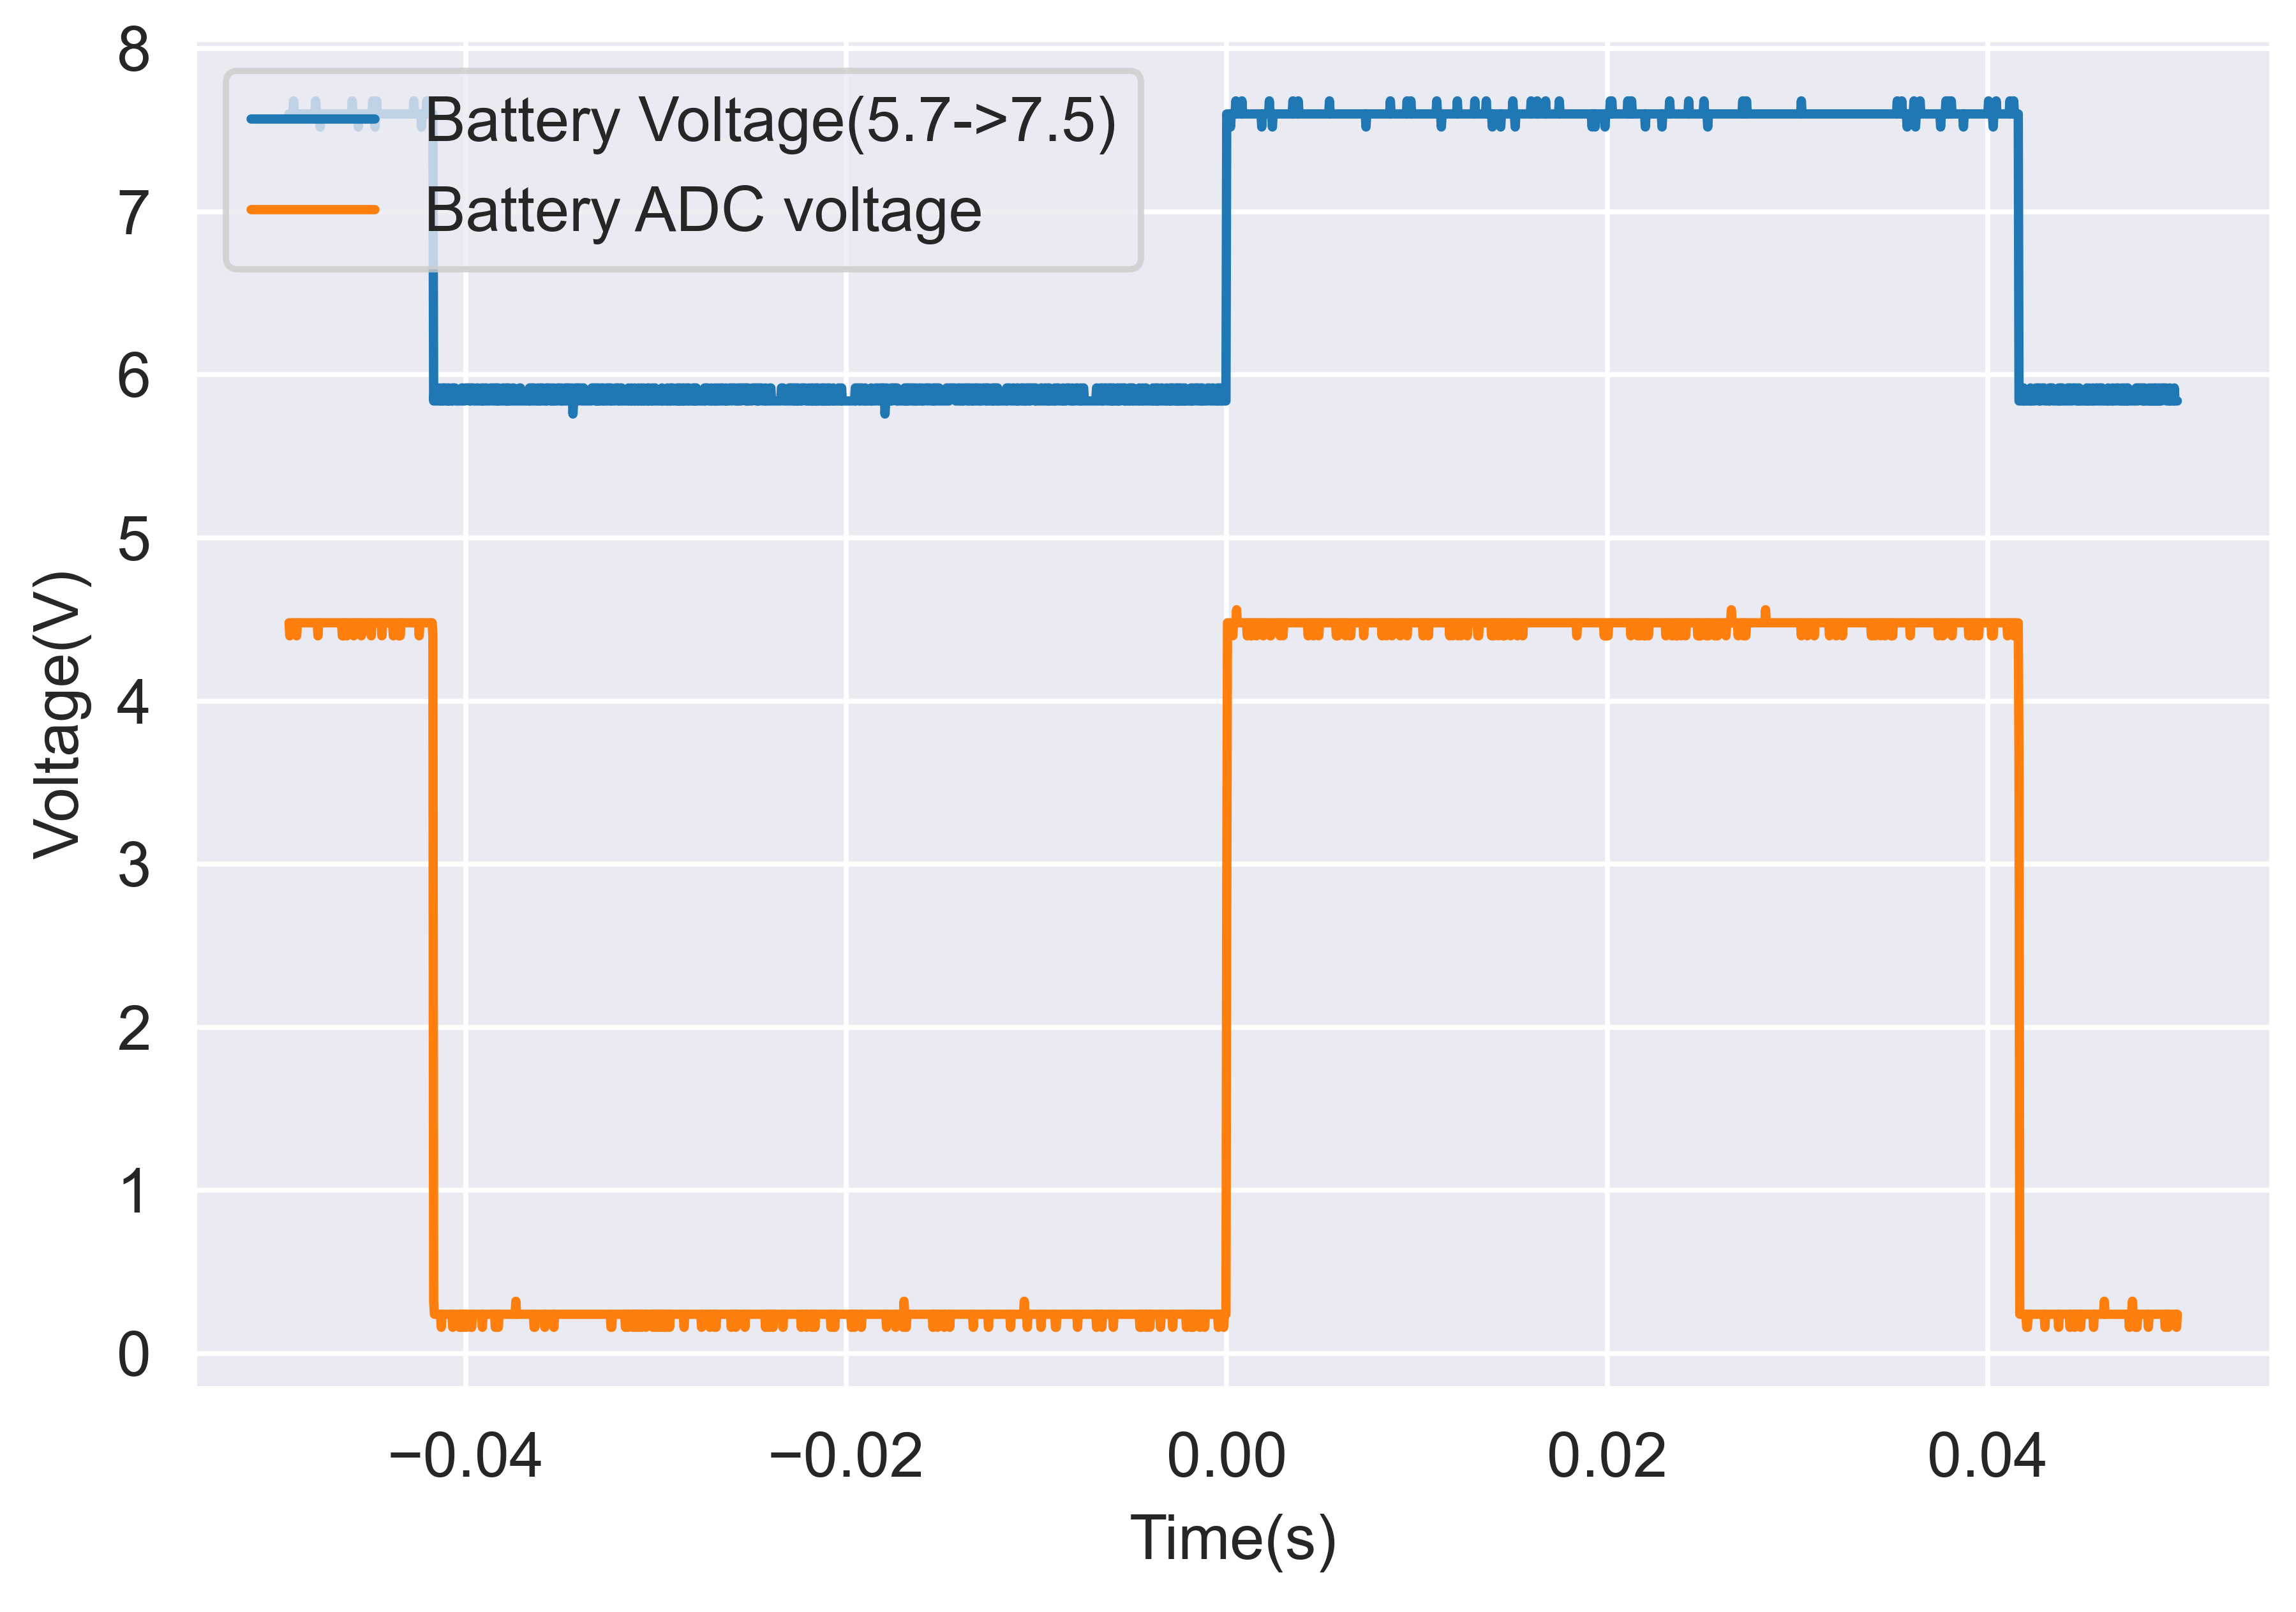
\includegraphics[scale=0.45]{./Figures/A6/batmeas.png}
	\caption{Oscilloscope data of rise time of battery voltage measuring circuit}
	\label{fig:batrise}
\end{figure}



\begin{table}[!htb]
	\centering
	\footnotesize
	\caption{Battery Measuring circuit measurements}
	\begin{tabular}{lrrrr}
		\toprule
		&Battery voltage& ADC Voltage&Expected ADC voltage& error \\
		&  [V]&[V]&[V]&[\%] \\
		\midrule
		&6&1.29&1.23  &4.88   \\
		&6.6&2.80&2.76  &1.45   \\
		&7.2&4.04&4.10   &1.46  \\
		\bottomrule
	\end{tabular}
	\label{tab:batmeas}
\end{table}


From figure \ref{fig:batrise} it can be seen that the rise time of channel 1 (ADC voltage) is practically instant and that the designed range is approximately achieved. Table \ref{tab:batmeas} represents the ADC voltage at the specific battery voltages and the error between the ADC voltage and the theoretical ADC voltage.









\chapter{System results}\label{chap:sysres}

\label{sec:sysRes}
The complete circuit charging characteristics are documented in table \ref{tab:batsys}. The current measurements are calculated from the TSC output using eq.\ref{eq:refeq}. A2 output refers to the output of the second assignment which can be seen in figure \ref{fig:under}. When comparing the tabulated results to graph \ref{fig:spiceReg} it can be said that these values are definitely comparable meaning that the practical circuit achieves its purpose.


\begin{table}[!htb]
	\centering
	\footnotesize
	\caption{Charging circuit measurements}
	\begin{tabular}{lrrrr}
		\toprule
		&Battery voltage while charging& Charging current&A2 output voltage \\
		&  [V]&[mA]&[V] \\
		\midrule
		&6.38&210&6.48     \\
		&6.42&192&6.51     \\
		&6.46&164&6.57     \\
		&6.53&152&6.60     \\
		&6.63&134&6.69     \\
		&6.64&132&6.7     \\
		
		
		\bottomrule
	\end{tabular}
	\label{tab:batsys}
\end{table}


With the circuit built up until this stage it was deemed necessary to recheck the hysteresis thresholds $V_{TU}$ and $V_{TL}$. From table \ref{tab:hyst meas} it can be seen that the thresholds are very close to the designed thresholds. The voltage following op amps likely stopped the external circuit from interfering with the voltages at the inputs of the op amps. 
\begin{table}[!htb]
	\centering
	\footnotesize
	\caption{Hysteresis Measurement}
	\begin{tabular}{lrrrr}
		\toprule
		& $Voltage$ \\
		&  [V] \\
		\midrule
		$V_{TU}$      & 6.22  \\
		$V_{TL}$     & 6.02\\
		
		\bottomrule
	\end{tabular}
	\label{tab:hyst meas}
\end{table}



\begin{figure}[!htb]
	\footnotesize
	\centering
	\begin{subfigure}[]{0.48\textwidth}
		\centering
		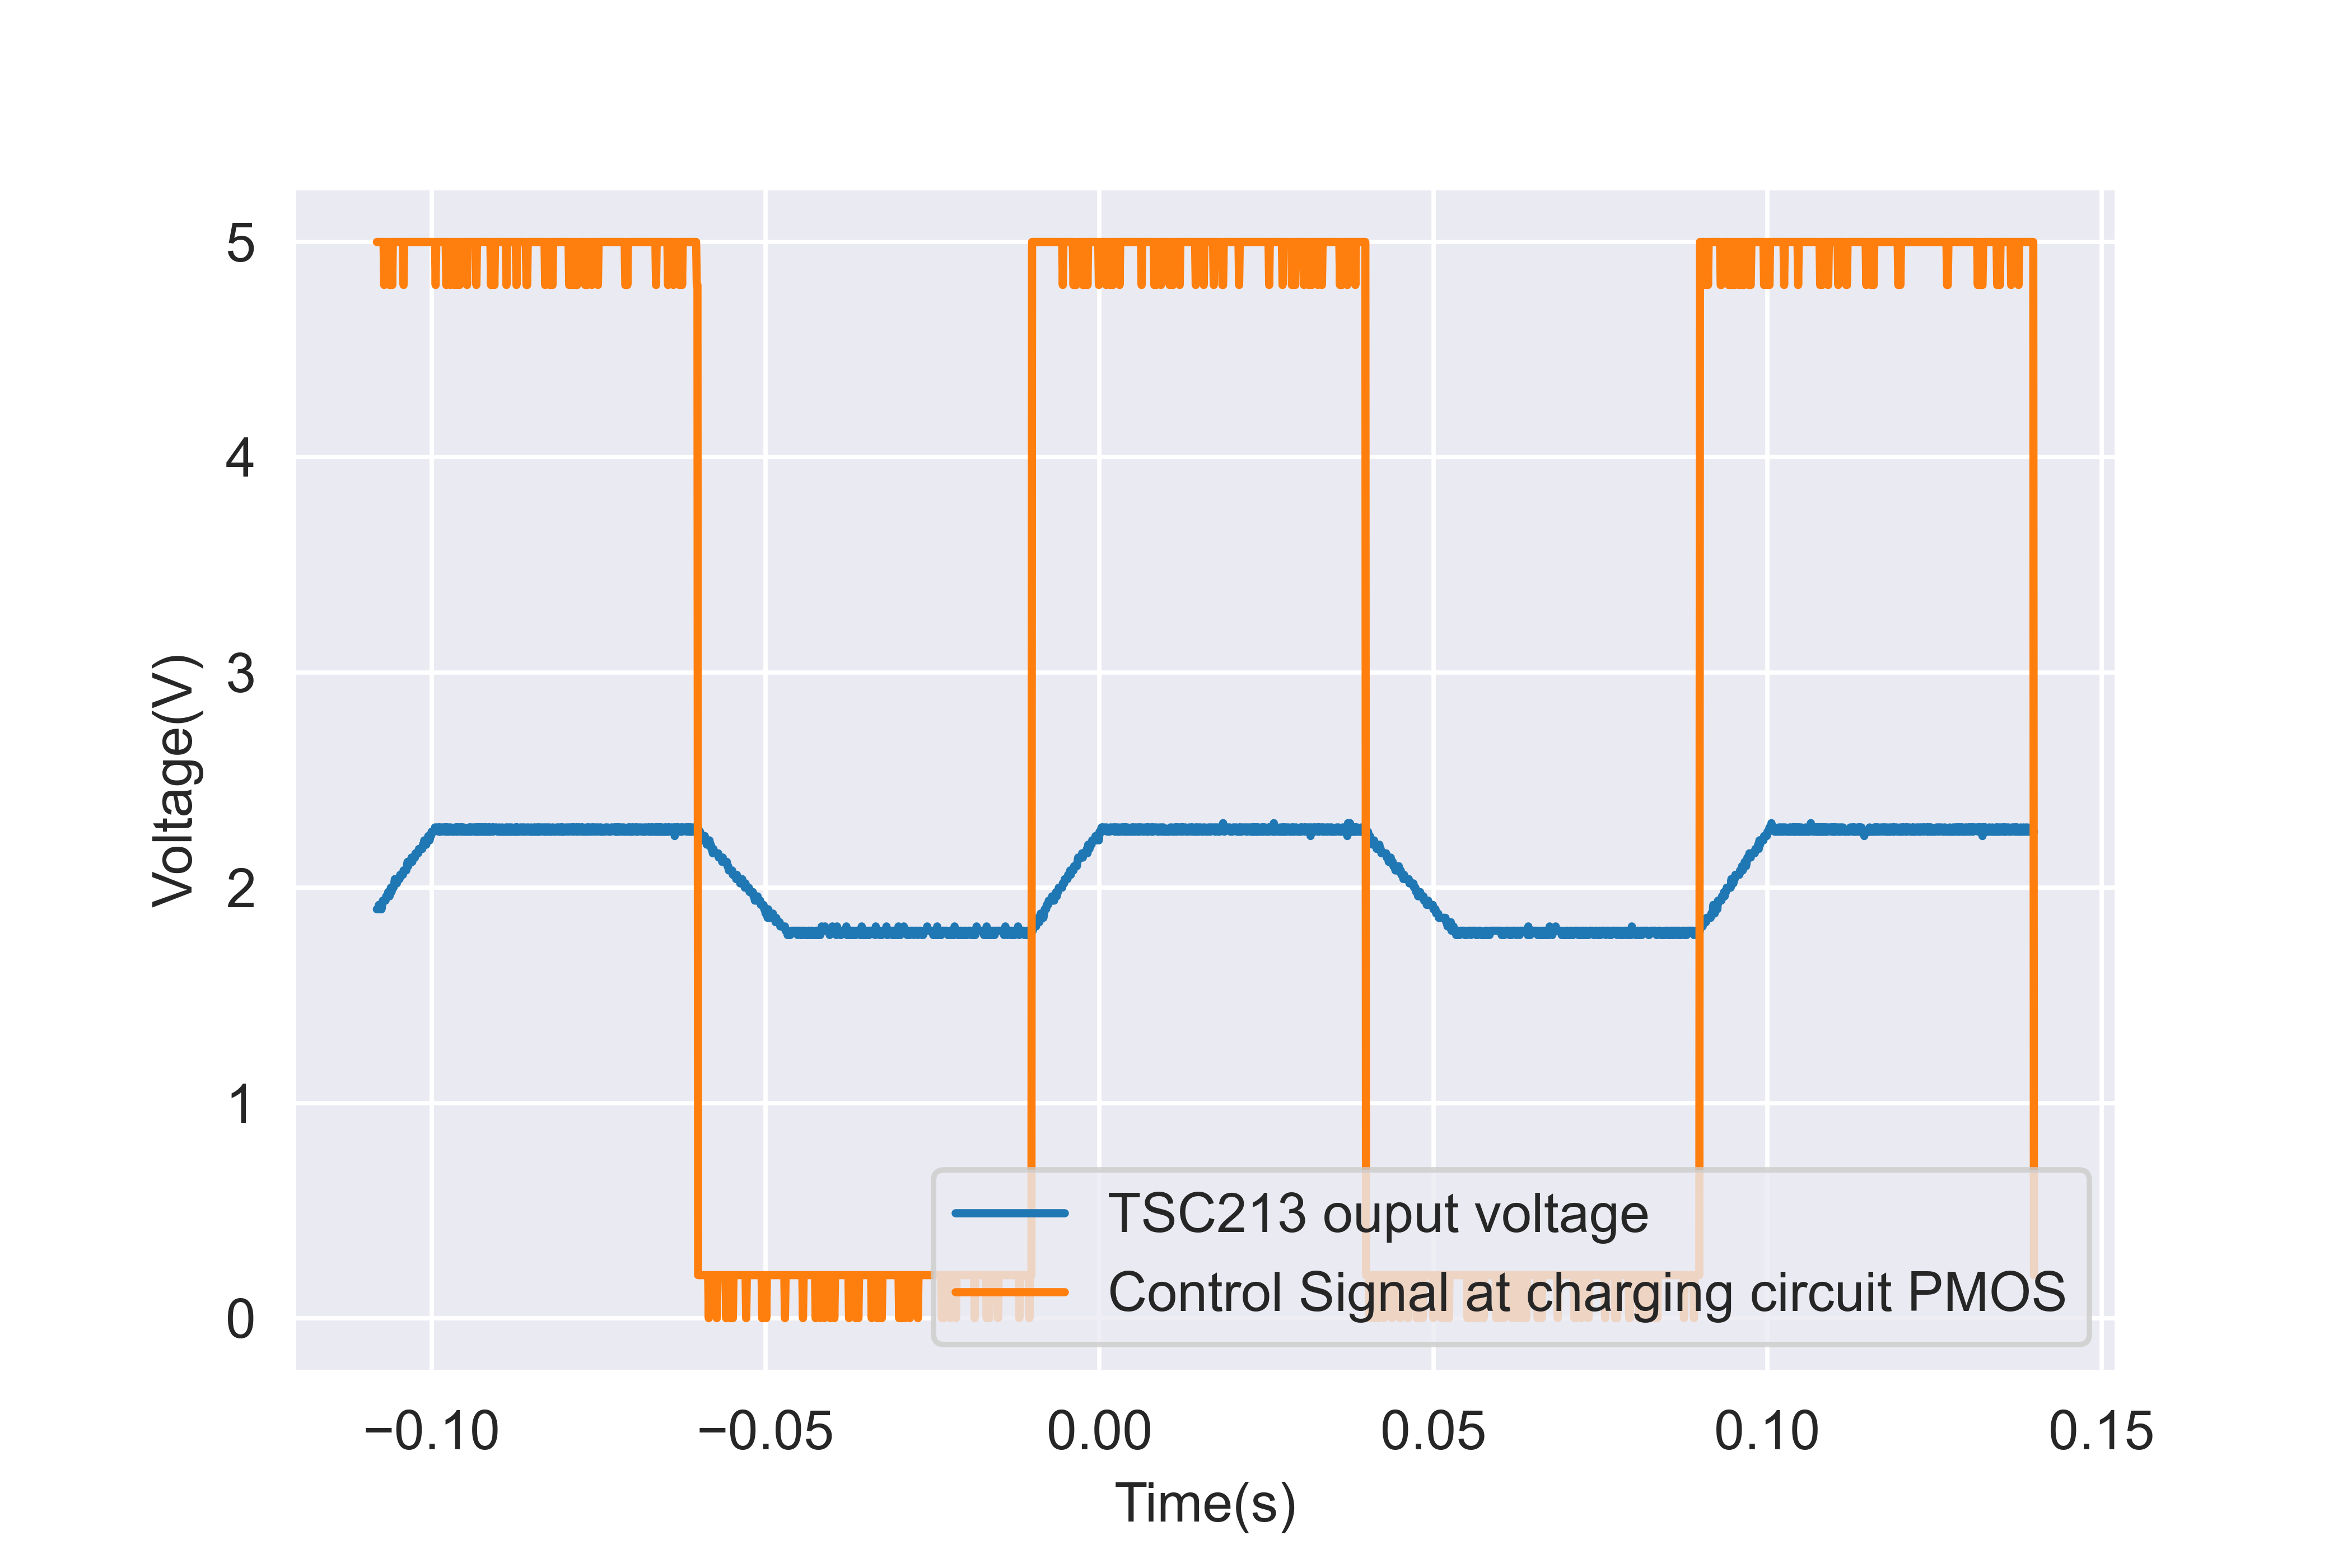
\includegraphics[width=1\linewidth]{./Figures/chargePMOSmeas}
		\caption{} \label{subfig:risePMOS}
	\end{subfigure}
	\begin{subfigure}[]{0.48\textwidth}
		\centering
		\includegraphics[width=1\linewidth]{./Figures/NMOSTSCmeas}
		\caption{ } \label{subfig:riseNMOS}
	\end{subfigure}
	\caption[{Rise Time for different switches }]{Oscilloscope switch evaluation of in system  (a)  High Side switch used to change TSC output  (b)Low side circuit used to change TSC213 output }
	\label{fig:rise}
\end{figure}

From the 2 figures in figure \ref{fig:rise} it can be said that the switches worked effectively in conjunction with the battery under voltage and charging circuits because as each switched changed state current discharged (NMOS ON, TSC output is below 1.75V) or charged (PMOS ON TSC output is above 1.75V). From these graphs it can also be seen that the time it takes for the output to change is less than 20 milliseconds which is fast.


\begin{figure}[!htb]
	\centering
	\includegraphics[width=0.85\linewidth]{Figures/numx.png}
	\caption{Circuit with barcode and Student Card}
	\label{fig:required}
\end{figure}
% Bibliography
\bibliography{References}


% End matter
\appendix
\chapter{GitHub Activity Heatmap}
\makeatletter\@mkboth{}{Appendix}\makeatother
\label{appen:github_heatmap}


     \begin{figure}[!htb]
     \centering
     	\fbox{\includegraphics[width=1\linewidth]{./Figures/gitHub.png}}
	\label{fig:github}
	\end{figure}
     \chapter{Data sheet info}

\begin{figure}[!htb]
\centering
\includegraphics[scale=0.5]{./Figures/datasheet}
\caption{tsc213 data sheet information}
\label{fig:data}
\end{figure}


\begin{figure}[!htb]
\centering
\includegraphics[scale=0.35]{Figures/circuitSTM.png}
\caption{Application Circuit For LM317\cite{STM}}
\label{fig:app}
\end{figure}




\begin{table}[!htb]
        \centering
        \footnotesize
        \caption{Thermal Resistance Values \cite{sink}\cite{STM}}
         \begin{tabular}{lrrrr}
          \toprule
             & $Thermal Resistance$ \\
             &  [\textdegree C/W] \\
          \midrule
          $\theta_{j-c}$ & 5      \\
          $\theta_{s-a}(worst case)$ &  20     \\
          $\theta_{j-a}$ &  50     \\

          \bottomrule
        \end{tabular}
     \label{tab:Thermal values}
\end{table}


\chapter{Additional Info}
\begin{figure}[!htb]
\centering
\includegraphics[scale=0.7]{./Figures/schmidt}
\caption{Non inverting Schmidt trigger\cite{Schmidt}}
\label{fig:schmidt}
\end{figure}




\end{document}

